\documentclass{svmult}

\usepackage[utf8]{inputenc}
\usepackage[usenames]{color}
\usepackage{url}
\usepackage{hyperref}

\usepackage[numbers]{natbib}
%\usepackage[switch]{lineno}

\usepackage{amsmath} % assumes amsmath package installed
\usepackage{amssymb}  % assumes amsmath package installed

\usepackage{enumerate}
\usepackage{paralist} %for inline lists

\usepackage{subfigure}

\usepackage{pseudocode}
\usepackage{alltt}

%diagrams
\usepackage{tikz}
\usetikzlibrary{shapes,trees}

\usepackage{lscape}

\usepackage[draft]{fixme}
\fxusetheme{color}

%%%%%%%%%%%% Custom macros %%%%%%%%%%%%%

%Name of the speaker in a chat
\newcommand{\chatN}[1]{{\footnotesize \textsf{#1}}}
\newcommand{\concept}[1]{{\footnotesize \texttt{#1}}}

\newcommand{\stmt}[1]{{\footnotesize $\langle$\stmttt#1\relax$\rangle$}}
\newcommand{\rawstmt}[1]{{\footnotesize \stmttt#1\relax}}
\def\stmttt#1 #2 #3\relax{{\tt#1} {\bf{\tt #2}} {\tt #3}}

\newcommand{\setstmt}[1]{{\footnotesize [\setstmttt#1\relax]}}
\def\setstmttt#1,#2\relax{\rawstmt{#1}, \rawstmt{#2}}

\newcommand{\ie}{{\textit{i.e.~}}}
\newcommand{\cf}{{\textit{cf~}}}
\newcommand{\eg}{{\textit{e.g.~}}}

%------------------------------------------------------------------------- 

\begin{document}
%\linenumbers

\title*{Towards Grounding Human-Robot Interaction}

\author{
Séverin Lemaignan,
Rachid Alami,
Amit Kumar Pandey,
Matthieu Warnier,
Julien Guitton
}
\authorrunning{Séverin Lemaignan et al.}

\institute{ 
	Séverin Lemaignan, \and Rachid Alami \and Amit Kumar Pandey \and Matthieu Warnier \and Julien Guitton
	\at
	CNRS - LAAS, 7 avenue du Colonel Roche, F-31077 Toulouse, France\\
	Université de Toulouse, UPS, INSA, INP, ISAE, LAAS, F-31077 Toulouse, France\\
	\email{surname.name@laas.fr}
}

\maketitle

\listoffixmes

\clearpage

\setcounter{minitocdepth}{2}
\dominitoc


\begin{abstract}
Abstract. 
\end{abstract}




%%%%%%%%%%%%%%%%%%%%%%%%%%%%%%%%%%%%%%%%%%%%%%%%%%%%%%%%%%%%%%%%%%%%%%%%%%%%
%%%%%%%%%%%%%%%%%%%%%%%%%%%%%%%%%%%%%%%%%%%%%%%%%%%%%%%%%%%%%%%%%%%%%%%%%%%%


\section{Grounding Human Interaction}

%\subsection{Situated speech acts}
%\label{intro_example}

{\em A messy table, covered with cardboard boxes, books, video tapes... Thomas
is moving out and is packing everything with the help of Jido, his robot.
``Jido, give me that'', says Thomas while looking at a box that contains a
video tape. The robot smoothly grasps the tape, and hands it to him.}

\begin{figure}%[!ht] 
	\centering
	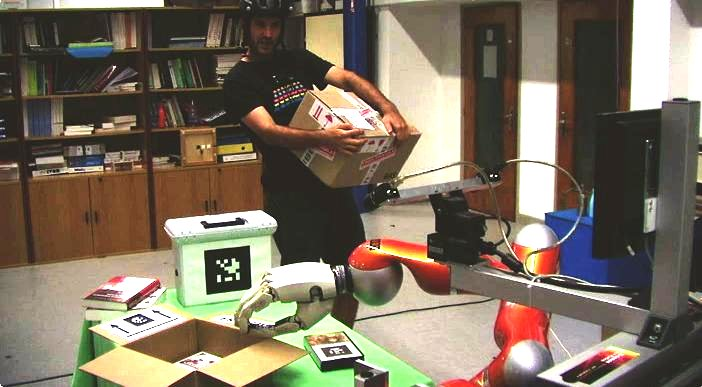
\includegraphics[width=1.0\linewidth]{figs/pt.jpg} 
	\caption{Interacting with
	the robot in an everyday setup: the human asks for help in vague terms, the
	robot takes into account the human's spatial perspective to refine its
	understanding of the question.} 
	\label{fig|vpt} 
\end{figure}


While this kind of interaction (Fig.~\ref{fig|vpt}) should hopefully sound
quite familiar in a foreseeable future, our robots are not yet quite up to the
task, neither regarding natural language understanding nor plan-making and
manipulation.  To be combined together, those abilities require an unambiguous
and shared representation of concepts (objects, agents, actions...) underlying
the interaction: what are the prerequisites for such a sentence --``Jido, give
me that''-- to be understood by the robot, correctly interpreted in the spatial
context of the interaction, and eventually transformed into an action?

The first step is to understand the meaning of the sentence. To this end, we
must acquire the sentence, convert it into a useful syntactic form (probably
through speech recognition), and understand the semantics of the sentence, \ie
What is referred by ``\textit{Jido}''? What is ``\textit{give}''? What is
``\textit{me}''? And ``\textit{that}''?

Working in a situated context, we need to \emph{resolve} these semantics atoms,
\ie ground them in the sensory-motor space of the robot. For instance,
``\textit{that}'' is a demonstrative pronoun that refers in this context to the
object the human is focusing on.

The next step is to extract and understand the \emph{intended meaning} of the utterance
as thought by the agent. In our example, Thomas obviously wants an action to be
performed by the robot. The action parametrization is conveyed by the semantics
attached to the words and the grammatical structure of the sentence. In our
example, the type of action is given by the verb ``\textit{give}''. Assuming
the robot has some procedural knowledge attached to this symbol, the action
type can be considered as grounded for the robot. We can as well understand
that the recipient of the action is the human, the performer is the robot
itself, and the object acted upon is the tape. The recipient, performer and object are three of the
\emph{thematic roles}~\cite{Gruber1965} that qualify the \emph{give} action. They are necessary to fully ground the sentence\footnote{This analysis has been
inspired on the work of Austin et al.~\cite{Austin1962}, where this type of
sentences correspond to \emph{speech acts}, comprising of \emph{locutionary
act} (the meaning), \emph{illocutionary} (the intent) and possibly
\emph{perlocutionary acts} (implicit speaker's expectation).}.


%\footnote{The third class of speech acts, the \emph{perlocutionary acts}, deal
%with implicit speaker's expectations. We will not consider it further in this
%article}.
%Austin~\cite{Austin1962} would have at first glance analyzed this kind of
%sentence as a \emph{speech act}, comprising of \emph{locutionary},
%\emph{illocutionary} and possibly \emph{perlocutionary} acts. 
%Firstly, we want to understand the direct meaning of the sentence (\emph{locutionary act}): 
%Second, the \emph{illocutionary force}, \ie the \emph{intent} of the utterance
%as thought by the agent, must be extracted and understood. 
%Finally, the implicit speaker's expectation can sometimes be conveyed --the
%\emph{perlocutionary act}-- and should be taken into account. If Thomas would
%have said instead ``Jido, this box is too heavy for me'', he may implicitly
%expect the robot to memorize the fact that the box's weight is over his
%capabilities, and it may as well imply that Thomas is requiring help to carry
%the box.

\subsection{A typical human-robot interaction problem}\label{sec:problem}

\fxfatal{Merge the section with previous one}

Let us consider a robot which is supposed to achieve interactive
object manipulation, fetch and carry tasks and similar tasks in a
domestic environment. The problem we are dealing with here is the
following. Given:
\begin {itemize}
\item a joint goal, which has been previously established and agreed
  upon (through a process which is out of the scope of this paper),
\item the current situation, acquired through perception or
  deduction from previous perceptions, including the state of the
  environment of the robot and of the human,
\end {itemize}
the robot controller computes an action to execute and who (the 
human or the robot, or both in case of a joint action) has to perform
it, and then controls or monitors its execution. The operation
continues until the goal is achieved, is declared unachievable or is
abandoned by the human.

To do so, the robot has to be equipped with a number of decisional, planning
and interpretation abilities where its human partner is taken
explicitly into account. It needs to be able:
\begin {itemize}
\item to build and maintain relevant robot and human beliefs
  (from the robot perspective) with respect to state of the world and the task,
\item to build and maintain iteratively shared (human-robot) plans, 
\item to refine and execute the actions it has to perform, and to monitor 
those achieved by its human partner.
\end {itemize}

Besides, we would like to build such abilities in a generic way, and
to provide several levels of parametrization allowing to adapt to
various environments, and various levels of involvement of the robot
ranging from teammate behavior to assistant or proactive helper.

\subsection{Approach}

In this work we propose an approach aiming at grounding the interaction with
users (Figure~\ref{fig|overall-process} illustrates the general context). To this end, we have
developed three distinct, inter-related cognitive components:

\begin{inparaenum}[\itshape 1)]

\item \emph{Physical environment modeling} and \emph{spatial reasoning}
(grouped under the term \emph{situation assessment}): this component is in
charge of building and maintaining a coherent model of the physical world. This
model is realistic in the sense that it relies on accurate 3D models of both
manipulable objects and humans. It also has dedicated mechanisms to manage
disappearing or occluded objects.  The geometric model is used to compute
several spatial properties of the scene that actually convert the original
sensory data into symbolic beliefs, including relative locations of objects,
visibility state, gestures (such as pointing), etc.  Assuming that other agents
are also represented in the model, the same computations are applied to analyze
the scene from each agent's point of view (\ie from their \emph{perspectives}).

\item \emph{Knowledge representation and management}: the robot is endowed with
an active knowledge base that provides a symbolic model of its beliefs of the
world, as well as models for each cognitive agent the robot interacts with.
Used in combination with the situation assessment framework, this proves an
essential feature (\cite{Roy2005,Kruijff2010}) to enable perspective-aware
grounding of natural language.

Our platform relies on OWL-DL\footnote{\emph{Web Ontology Language -
Description Logics}, a decidable subset of the first-order logics,
\url{http://www.w3.org/TR/owl2-primer/}} ontologies and features continuous
storage, querying and event triggering over the pool of facts known by the
robot.

\item \emph{Dialogue processing}: the third component includes natural
language parsing capabilities, interactive disambiguation routines and concept
anchoring. We focused our efforts on three classes of utterances commonly found
in human-robot interaction: \emph{statements} (\ie new facts the human wants to
inform the robot), \emph{orders} (or more generically \emph{desires}) and
\emph{questions on declarative knowledge} (whose answers do not require
planning or prediction)\footnote{This would roughly cover the \emph{representative}
(sometimes referred as \emph{assertive}) and \emph{directive} illocutionary
acts in Searle's~\cite{Searle1976} classification.}.

\end{inparaenum}

\begin{figure}[!t]
\centering
  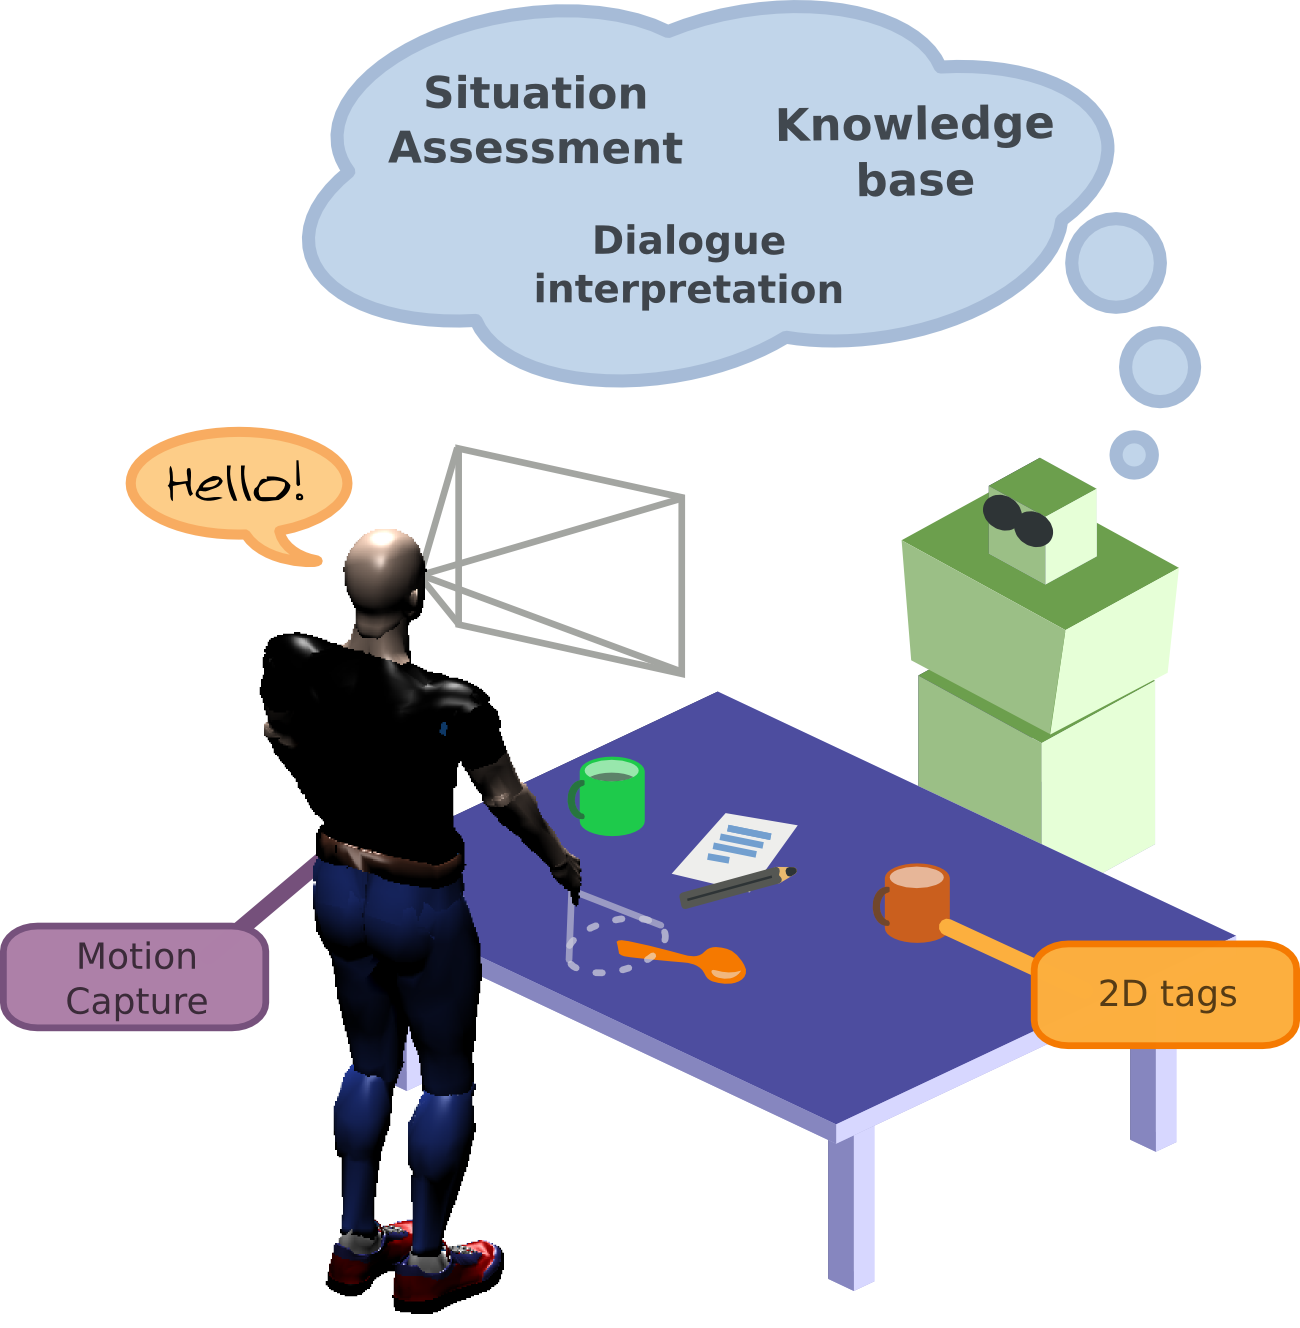
\includegraphics[width=0.8\linewidth]{figs/grounding_robot.png}
  \caption{Generic model of cognitive abilities interactions for grounding}
  \label{fig|overall-process}
\end{figure}

%\begin{figure}[!ht]
%\centering
%  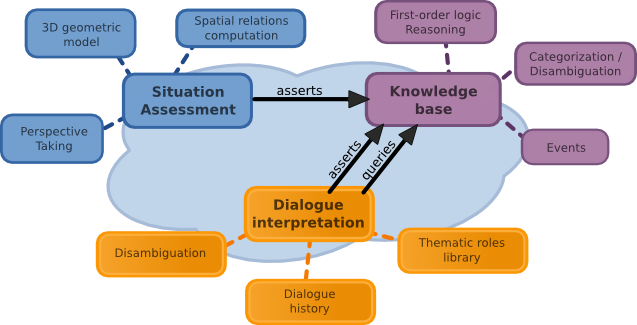
\includegraphics[width=0.9\linewidth]{figs/grounding.png}
%  \caption{The three main components of our architecture and their connections. Submodules are presented in subsequent sections.}
%  \label{fig|main-components}
%\end{figure}

%~ The system we describe here relies on two distinct activities that run concurrently and continuously: maintenance of a symbolic model from real world interpretation on one hand, and verbal interaction with agents on the other hand.
%~ 
%~ The first activity consists in two main steps:
%~ 
%~ \renewcommand{\labelenumi}{(\alph{enumi})}
%~ \begin{enumerate}
%~ \item The \emph{Object Identification} step is expected to provide consistent identification of objects in the environment. It does not involve any semantic functionality like automatic labelling, classification or annotation capabilities. It is in charge of solving what is merely a perception issue related to the ability to assign some identifier consistently. This is in the general case an open research issue that is outside of the scope of this paper. In our experiments, we will use simplified approaches (like tag-based object identification and motion capture).
%~ 
%~ Besides identification, other perceptual informations are extracted at this step, such as absolute size, color, and more importantly, its spatial position relative to the robot.
%~ 
%~ \item \emph{Physical environment modeling} and \emph{spatial reasoning} are then in charge of rebuilding a coherent physical model of the world based on information extracted in the first step. Once available, the geometric model is used to compute several spatial properties of the scene that actually convert the original sensory data into symbolic beliefs. This includes relative locations of objects, visibility state, gestures like pointing, etc. Assuming that other agents are as well represented in the model, the same computations can be applied to analyze the scene from each agents' point of view (\ie from their \emph{perspectives}).
%~ \end{enumerate}
%~ 
%~ The output of this second step needs to be stored for later reuse: we introduce to that end a general-purpose knowledge management system that relies on a sound logical system (the Description Logics) to store, manipulate and reason about symbolic knowledge. This system is described at length in the next section.
%~ 
%~ The verbal interaction activity relies on three main steps:
%~ 
%~ \begin{enumerate}
%~ \item The \emph{parsing} of natural language aimed at extracting grammatical structures from a sentence,
%~ 
%~ \item The \emph{resolution} of concepts, where words used by the user are associated with the underlying concept they represent, as stored in the robot knowledge base. This step may require an additional interactive disambiguation step if the robot can not successfully bind a word to the concept it represents.
%~ 
%~ \item Finally, the \emph{content analysis} step extracts the \emph{intention} of the sentence and handles it. Orders, questions, statements (new information) are separately processed.
%~ \end{enumerate}

\subsection{Related Work}

Our work builds on top of years of work in the artificial intelligence
community around the symbol grounding issue: we can mention
Searle~\cite{Searle1980} who introduces it with the \emph{Chinese room}
metaphor, Harnard~\cite{Harnad1990} who coins the following (slightly
paraphrased in the robotic context) definition of symbol grounding:
\emph{``make the meanings of the meaningless symbol tokens intrinsic to the
robotic system"}, Coradeschi and Saffioti~\cite{Coradeschi2003} who focus on
robotics and define the meaning of \emph{anchoring} as \emph{``the process of
creating and maintaining the correspondence between symbols and sensor data
that refer to the same physical object''} and Ziemke~\cite{Ziemke1999} who
elaborates on the need of embodiment for symbol grounding.

Our contribution relates to two narrower fields: natural language in embodied
interaction contexts and knowledge acquisition and representation in robotic
systems.

Processing natural language in situated contexts is already an established
research field. In~\cite{Roy2005}, Roy and Reiter summarize what they see as
the main challenges to be tackled: cross-modal representation systems,
association of words with perceptual and action categories, modeling of
context, figuring out the right granularity of models, integrating temporal
modeling and planning, ability to match past (learned) experiences with the
current interaction and ability to take into account the human perspective.
This list offers an interesting entry point to evaluate our contribution.

Kruijff et al. provides in~\cite{Kruijff2010} an up-to-date survey of
literature on situated human-robot dialogue, focusing on formal representation
systems, bi-directionality of the interaction and context building. They point
out as well that compared to the cognitive psychology community, the ``situated
AI'' community started only recently to take into account agents' focus of
attention, perspective and temporal projection abilities.

Dialogue processing in real robots have been explored by several teams.  Brick
and Scheutz~\cite{Brick2007} have contributions regarding natural language
processing in an incremental way, and how this enables instant back-channel
feedback (like nodding). Hüwel et al.~\cite{Huwel2006} propose the concept of
\textit{Situated Semantic Unit}: atoms are extracted from sentences exposing
semantic links to other units. The parser tries to satisfy these links and
rates the semantic interpretation of the sentence. Used in conjunction with
ontologies, their approach offers robustness to ungrammatical or partial
utterances. They validated the approach with an extensive user-study.

Zender et al.~\cite{Zender2009} address the generation of referring expressions
(GRE~\cite{Dale1995}) in situated dialogue for topological knowledge.  They consider
both the reference resolution and reference description tasks, and rely on
OWL-DL representation and SPARQL\footnote{{\em SPARQL Protocol and RDF Query
Language}, \url{http://www.w3.org/TR/rdf-sparql-query/}} to extract
\emph{topological contexts} from their knowledge base.

While mostly implemented on virtual agents, the GLAIR cognitive architecture by
Shapiro and Bona~\cite{Shapiro2009} is an architecture explicitly built to
tackle the grounding issue from the percept to the decision. It is a
three-layers architecture: a \emph{Knowledge Layer}, a low-level
\emph{Sensori-Actuator Layer} and an intermediate \emph{Perceptuo-Motor Layer}
that binds the previous two.  The knowledge layer relies on a custom knowledge
representation language (more expressive than first-order logic), and natural
language processing capabilities similar to ours are available. The GLAIR
project has been only demonstrated in a limited set of environments, but
exhibits interesting features such as explicit management of contexts of facts
and memory models (long term/short term, episodic/semantic).

Also worth mentioning, Mavridis and Roy~\cite{Mavridis2005} propose the idea of
a \emph{grounded situation model} which is an amodal model of the world where
different sensing modalities, including verbal ones (the robot is able to
\emph{imagine} objects), are merged. Their framework also allows the management of
the interaction history (the human can ask for a past event). They propose an
implementation in an environment built on simple entities (a manipulator arm
and colored balls).

In the field of symbolic knowledge processing for robots, Gunderson and
Gunderson~\cite{Gunderson2008} introduce the concept of \emph{reification}
(based on both recognition and pre-afference) as an intermediate step between
pattern recognition and symbol grounding. Their underlying storage of knowledge
relies on ontologies and bio-inspired memory models. While sharing similar
foundations to our work, their proposal is based on fairly simple perceptual
modalities and does not develop complex symbolic models that could enable
human-robot interaction.

Suh et al.~\cite{Suh2007} develop {\sc OMRKF}, an ontology-based reasoning
framework for robotics. They tackle the grounding problem by storing low-level
facts (like SIFT visual features) in a layered symbolic architecture that works
well in simple sensori-motor spaces. However this approach raises concerns
regarding scalability and management of more complex entities or interactions.

Daoutis et al.~\cite{Daoutis2009} introduce one of the first complete
architectures for grounded human-robot interaction. They successfully bind
low-level percepts (including view-point independent SIFT based object
recognition) to a high-level knowledge representation and reasoning system.
They base their knowledge model directly on the \textit{ResearchCyc} ontology
(including the \textit{MicroTheories} concept), used in combination with the
{\sc CycL} language. This enables second-order logic modeling and access to a
large common-sense knowledge base.

Beetz et al.~\cite{Beetz2010} proposes a cognitive architecture called
\textsc{CRAM} (Cognitive Robot Abstract Machine) that integrates
\textsc{KnowRob}~\cite{Tenorth2009a}, a knowledge processing framework based on
Prolog. Its underlying storage is based on an OWL ontology, derived from
\textsc{OpenCyc}. \textsc{CRAM} and \textsc{KownRob} have been demonstrated on
several real-world scenarios, where natural language recipes extracted from
Internet had to be translated into plans and executed in a kitchen environment,
perceived and rebuilt on-line by the robots. While Prolog offers more flexible
modeling (no constraints on the arity of predicate, where Description Logics as
used in our work are limited to binary predicates), it is based on the closed
world assumption (if something cannot be inferred to be true, it is inferred to
be false) whereas we rely on the open world assumption, which is more realistic
in real world scenarios. A probabilistic extension of \textsc{KnowRob}, called
\textsc{ProbCog}~\cite{Jain2009} is also available. While in principle
possible, currently the CRAM architecture does not provide explicit support for
interacting with humans.

\subsection{Related work and vision}\label{sec:soa}

\fxfatal{Merge the section with previous one}

The human presence brings new requirements for robot's abilities both
at the functional and at the deliberative levels~\cite{Klein2004}. The
topics involve motion~\cite{Kulic2007,Berg2004,Madhav2006},
navigation~\cite{Althaus2004,Sisbot2007}, manipulation~\cite{Kemp2007}
in presence of humans as well as perception of human
activities~\cite{Breazeal2001,Burger2008}. Also, when
interacting with humans, robots need to incorporate communication and
collaboration abilities. Several theories dealing with
collaboration~\cite{Cohen1991,Grosz1996,Clark1996} emphasize that
collaborative tasks have specific requirements compared to individual
ones, \eg, since the robot and the person share a common goal, they
have to agree on the manner to realize it, they must show their
commitment to the goal during execution, etc. Several robotic systems
have already been built based on these
theories~\cite{Rich1997,Sidner2005,Tambe2005a,Breazeal2003} and they
all have shown benefits of this approach. They have also shown how
difficult it is to manage turn-taking between communication partners
and to interleave task realization and communication in a generic
way. Finally, today only few
systems~\cite{Fong_2006,Breazeal2003,Sisbot2008} take humans into
account at all levels.

Perspective Taking is a human ability which allows one to put
him/herself in another person's point of view. Studied in
psychology literature~\cite{Flavell1992,Tversky1999}, this ability is
crucial when interacting with people by allowing one to reason on
others' understanding of the world in terms of visual perception, spatial
descriptions, affordances and beliefs, etc.
Therefore, in the last years these notions have been gradually
employed in Human-Robot Interaction.~\cite{breazeal2006} presents a
learning algorithm that takes into account information about a
teacher's visual perspective in order to learn a
task. ~\cite{Johnson2005} apply visual perspective taking for action
recognition between two robots.~\cite{Trafton2005} use both visual and
spatial perspective taking for finding out the referent indicated by a
human partner.

Spatial reasoning~\cite{OKeefe1999}, on the other hand, has been used
for natural language processing for applications such as direction
recognition ~\cite{Kollar10,Matuszek10} or language
grounding~\cite{Tellex10}.~\cite{Skubic2004} presented a spatial
reasoner integrated in a robot which computes symbolic positions of
objects.

\begin{figure}[htb]
\centering
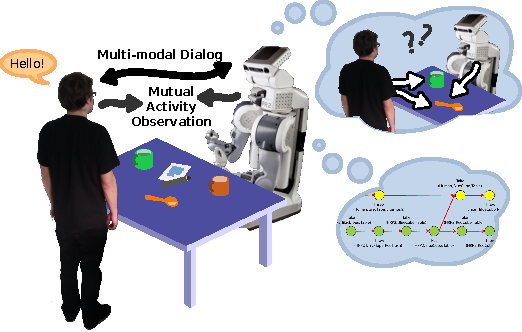
\includegraphics[width=9cm]{figs/grounding_robot.pdf}
\caption{Robot reasoning about HRI and anticipation of human activities:
  sources of information are multi-modal dialogue, and observation of
  environment and human activity}
\label{fig:hri-dec}
\end{figure}

We envision HRI in a context where two agents (a human and a robot)
share a common space and exchange information through various
modalities. Our aim is to endow the robot with an explicit
consideration of the human and with the ability to manage its
interactions with him (Figure~\ref{fig:hri-dec}). This must be
considered at the architecture level as well as at the task/motion
planning and execution level. 

We have devised a decisional framework for human-robot interactive
task achievement that is aimed to allow the robot not only to
accomplish its tasks but also to produce behaviors that support its
engagement vis-a-vis its human partner and to interpret human
behaviors and intentions. 
Together and in coherence with this framework, we have developed
and experimented various task planners and interaction schemes that
allow the robot to select and perform its tasks while taking into
account explicitly the human abilities as well as the constraints
imposed by the presence of humans, their needs and preferences. 


%\subsection{Contributions}

%Besides proposing a new integration model for sensor data, natural language and
%symbolic knowledge repositories, our work extends these previous contributions
%by tackling more realistic human-robot interactions: less restricted speech
%understanding; ability to deal with complex, partially unknown human
%environments; and fully embodied (with arms, head,...) autonomous robots that
%manipulate a large range of household objects.

%Three specific contributions are presented in this work: first, we introduce a
%versatile and light-weighted knowledge base that models in a formal framework,
%based on first-order logics, not only the robot's own beliefs but also every
%other cognitive agent the robot interacts with.  This explicit modeling of
%other agents' belief states is used for the interaction and eases the
%implementation of various advanced cognitive behaviors like
%False-Beliefs~\cite{Leslie2000} or interactive object discrimination.

%Second, we have implemented a framework to extract symbolic facts from complex
%real scenes. It is based on a 3D model of the world that the robot builds
%on-line by merging different sensor modalities. It computes spatial relations
%between perceived objects in real-time and it allows for virtually \emph{viewing}
%of the same scene from different points of view, enabling \emph{visual} and
%\emph{spatial agent perspective taking}.

%Third, the same symbolic knowledge base enables richer language capabilities
%for the robot.  We propose a new approach to natural language grounding that is
%robust, situated and more generic than what can be found in previous work
%on situated language grounding. We present several examples that include
%recognition and semantic validation of thematic roles or disambiguation
%based on attention foci.

%Communcation between these components is build as streams of symbolic facts,
%where knowledge manipulated by the robot is made explicit.
%This leads us to the idea of a \emph{knowledge-oriented architecture}, which is
%discussed at the end of the article.

%These points highlight some original aspects of a larger cognitive architecture
%that has been deployed and tested on several mobile robotic platforms
%(including both humanoid robots and service robots), demonstrating the
%versatility and hardware-agnosticism of these developments.

\subsection{Chapter overview}

In the next section we present the {\sc ORO}
(\emph{OpenRobots Ontology} server) knowledge base. We present it first, along with its objectives,
since it is the knowledge \textit{hub} of the system, used pervasively by other
components.
Section~\ref{spark} presents {\sc SPARK} (for \emph{SPAtial Reasoning \& Knowledge}), the
component that merges perceptual information with a coherent geometric model and
builds a symbolic interpretation of the world from the robot's point of view,
as well as an individual symbolic model for each agent currently present in the
environment. 
Section~\ref{dialog} covers in detail the dialogue processing component and its 
relation with ORO.
Section~\ref{experiments} presents three use-cases that were conducted on two 
different robotic platforms: the \emph{Naming} experiment, where a robot anchors new
knowledge in its model through verbal interaction; the \emph{Spy Game}, where
either the user or the robot tries to guess which object the other player is
thinking of; and a more complex experiment situated in an everyday setup, where
the robot builds models for several agents and interacts with the users using
this knowledge. 
Finally, Section~\ref{conclusion} concludes and discusses the work presented 
in this paper.






%%%%%%%%%%%%%%%%%%%%%%%%%%%%%%%%%%%%%%%%%%%%%%%%%%%%%%%%%%%%%%%%%%%%%%%%%%%%
%%%%%%%%%%%%%%%%%%%%%%%%%%%%%%%%%%%%%%%%%%%%%%%%%%%%%%%%%%%%%%%%%%%%%%%%%%%%

\section{An architecture for grounding}
\label{sec:Framework}

Interaction happens as a consequence of an explicit request of the
human to satisfy a goal or because the robot finds itself in a
situation where it is useful if not mandatory. In both cases, the
robot has a goal to satisfy.  An important issue is the notion of
engagement, a process in which the robot will have to establish,
maintain and terminate a connection with a human partner. 
This covers goal establishment, selection of an incremental refinement
of the task that is intended to be achieved, and execution control
including monitoring, and even influencing, human task performance and
his/her commitment to the goal. The human involvement may range from a
direct participation to the task achievement, to a simple
``acceptance'' of robot activity in his/her close vicinity.
  
Our robot is controlled by a three layer
architecture~\cite{Alami1998}.  We present briefly its decisional
layer. The proposed decisional framework consists of several entities,
having each a specific role as illustrated by
Figure~\ref{architecture_fg}.  We describe how the robot is controlled
through an analysis of the three main activities performed by the
robot controller:

\begin{figure*}[thpb]
  \centering
  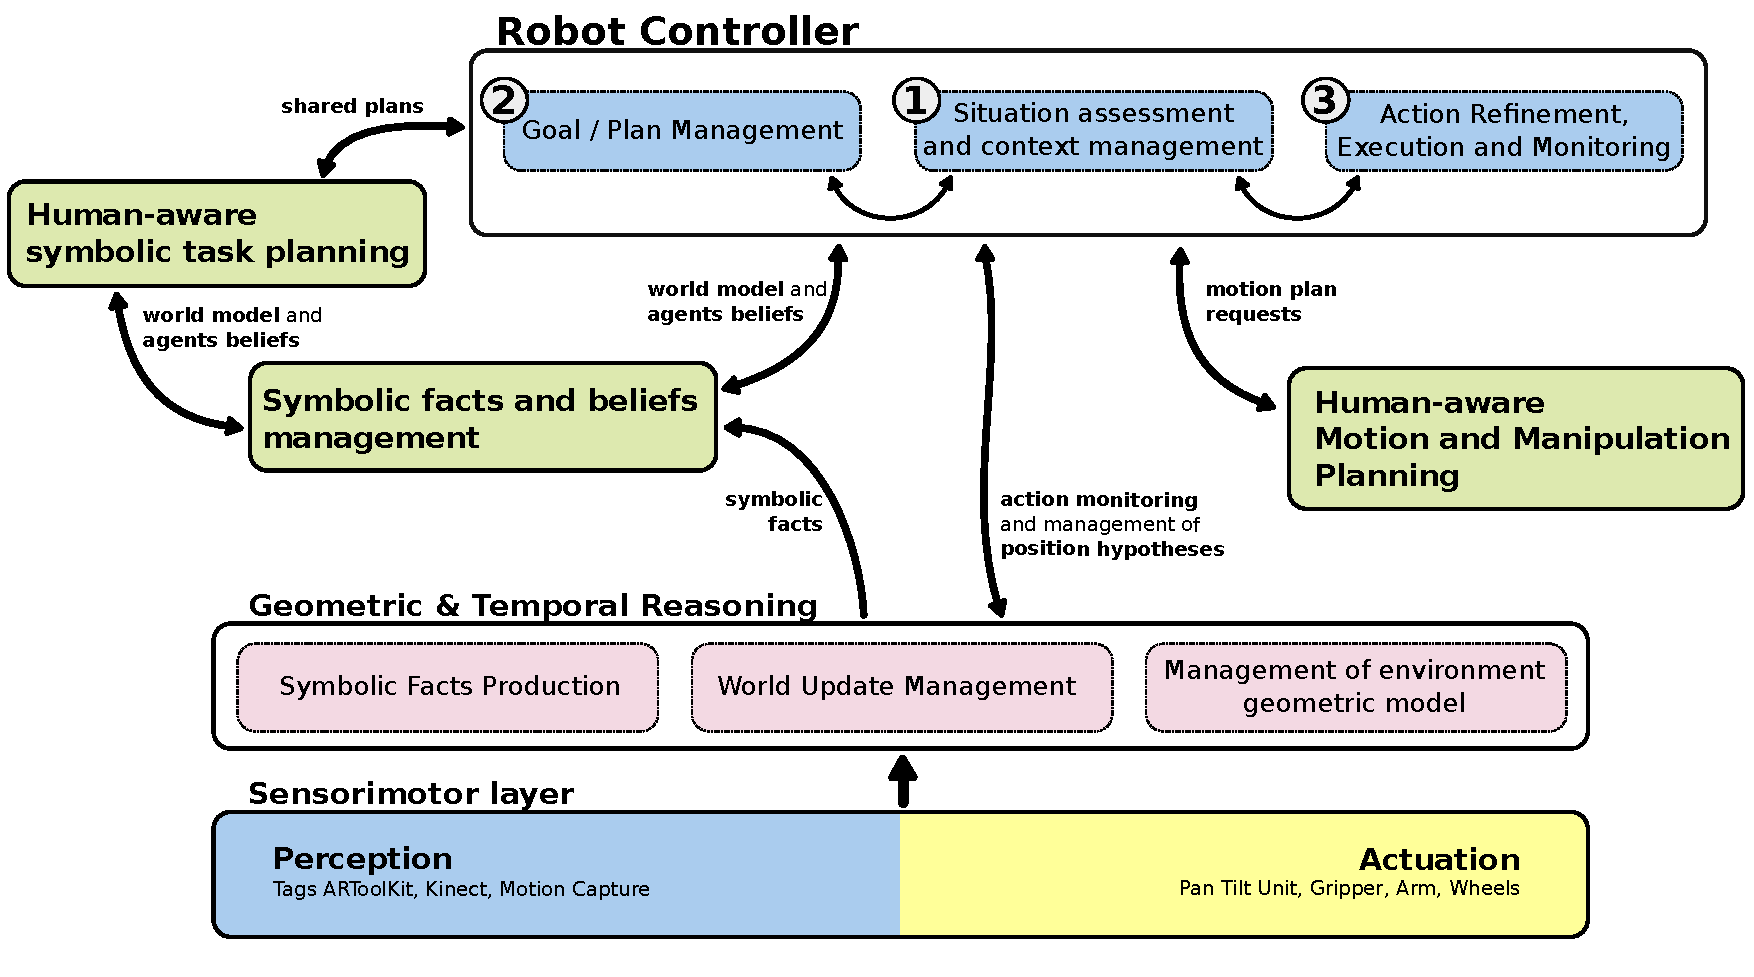
\includegraphics[width=1.0\textwidth]{./figs/supervisor-architecture-new.pdf} \\
  \caption {Architecture of the robot control system}
  \label{architecture_fg}
\end{figure*}

\begin {enumerate}
\item Situation assessment and context management 
\item Goals and plans management
\item Action refinement, execution and monitoring
\end {enumerate}

The next three sections describe the three robot controller
activities and how they make use of a number of key components in the
architecture:

\begin{itemize}
\item SPARK: Spatial Reasoning and Knowledge module \cite{Sisbot2011}
\item ORO: a knowledge management module \cite{Lemaignan2010}
\item HATP: a Human-Aware Task Planner \cite{Alili2008}
\item A set of Human aware motion, placement and manipulation planners
 \cite{Sisbot2008, Mainprice2011, Pandey2010}
\end{itemize}

Other decisional activities, such as situated dialog (\cite{Ros2010b,
  Lemaignan2011}, not presented here) have been developed that use the
same set of components.






%%%%%%%%%%%%%%%%%%%%%%%%%%%%%%%%%%%%%%%%%%%%%%%%%%%%%%%%%%%%%%%%%%%%%%%%%%%%
%%%%%%%%%%%%%%%%%%%%%%%%%%%%%%%%%%%%%%%%%%%%%%%%%%%%%%%%%%%%%%%%%%%%%%%%%%%%

\section{Situation assessment and context management}
\label{sec:situ}

\fxfatal[author=Severin]{Review/reorganize this section.
Add a section on Migthabilities Maps as well (keeping in mind the paper must
focus on link between continous and symbolic worlds)}

This activity involves the geometric and temporal reasoning component,
the symbolic facts and belief management component and the dedicated
robot controller activity (Figure~\ref{architecture_fg}).

We assume that perception provides in real-time the identity and the
position of objects when they are in the field of view of the sensors.
In our implemented examples, the robot is localised using a standard
horizontal laser-scanning based localisation system, the objects are
identified and localized using ARToolkit \cite{ARToolkit} and the
humans are tracked using a commercial motion capture system and a
Kinect device from Microsoft.

\subsection{Geometric and Temporal Reasoning component}\label{sub:gtrc}

The geometric reasoning component plays a central role in our
architecture. It is called SPARK (Spatial Reasoning and
Knowledge~\cite{Sisbot2011}) in the current implementation. It is
responsible for geometric information gathering and it embeds a number
of decisional activities linked to abstraction (symbolic facts
production) and inference based on geometric and temporal reasoning.
SPARK maintains all geometric positions and configurations of agents,
objects and furniture coming from perception and previous or {\it a
  priori} knowledge.

 %\subsubsection*{Symbolic facts production:} 
\vspace{0.3cm}
\noindent
\textbf{Symbolic facts production:} 
Geometric state of the world is abstracted in symbolic facts that can
be classified in three different categories.

\begin {itemize}
\item Relative positions of object and agents, e.g.  \stmt{GREY\_TAPE
    isOn TABLE}.

\item Perception and manipulation capacity and state of agents,
  e.g. \stmt{ROBOT looksAt GREY\_TAPE}, \stmt{GREY\_TAPE isVisibleBy
    HUMAN1}.

\item Motion status for object or agent parts, e.g.  \stmt{GREY\_TAPE
    isMoving true},\\ \stmt{ROBOT\_HEAD isTurning true}.
\end {itemize} 

Reasoning about human perspective allow to compute facts such as:
\stmt{GREY\_TAPE isBehind HUMAN1}, \stmt{GREY\_TAPE isVisibleBy
  HUMAN1}.

Figure~\ref{fig::reach-ex} illustrates different situations for the
\textit{reachable} relation. In this case, the robot and its human partner
are placed face to face, in a table-top setup (Figure~\ref{fig::reach-ex}.1).
The robot first estimates if the small grey box is reachable to itself. This is
done by finding a collision free posture to reach the object
(Figure~\ref{fig::reach-ex}.2). Next the robot switches to the human's
perspective to estimate if the same object is reachable to the human as well.
In the last scene, the human moves towards his left, farther from the object
(Figure~\ref{fig::reach-ex}.4). The situation is then reevaluated. In this
occasion though, the reasoner cannot find a satisfactory posture for the human
to reach the box because he is too far from the target.

\begin{figure*}[!t]
	\centering
	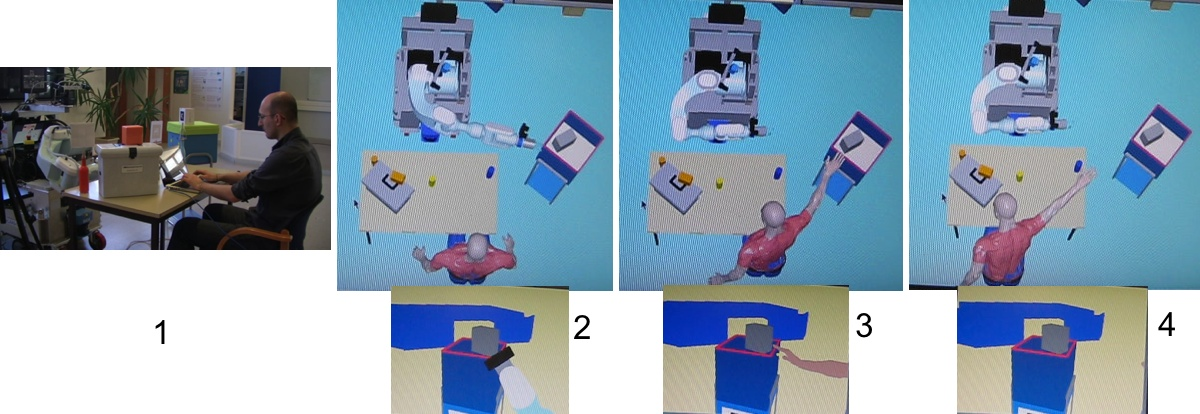
\includegraphics[width=1.0\textwidth]{figs/reachex.jpg}	
	\caption{An example illustrating the \textit{reachable} relation. The relation is computed from the perspectives of both the robot and the human. The computed posture at each step is illustrated with a global view of the scene (top), and from a closest view (bottom).}
\label{fig::reach-ex}
\end{figure*}

\begin{figure}[ht!]
   \label{fig:sparkSubfigures}
   \begin{center}
%
       \subfigure[Initial state]{%
%           \label{fig:wuweiPhoto}
           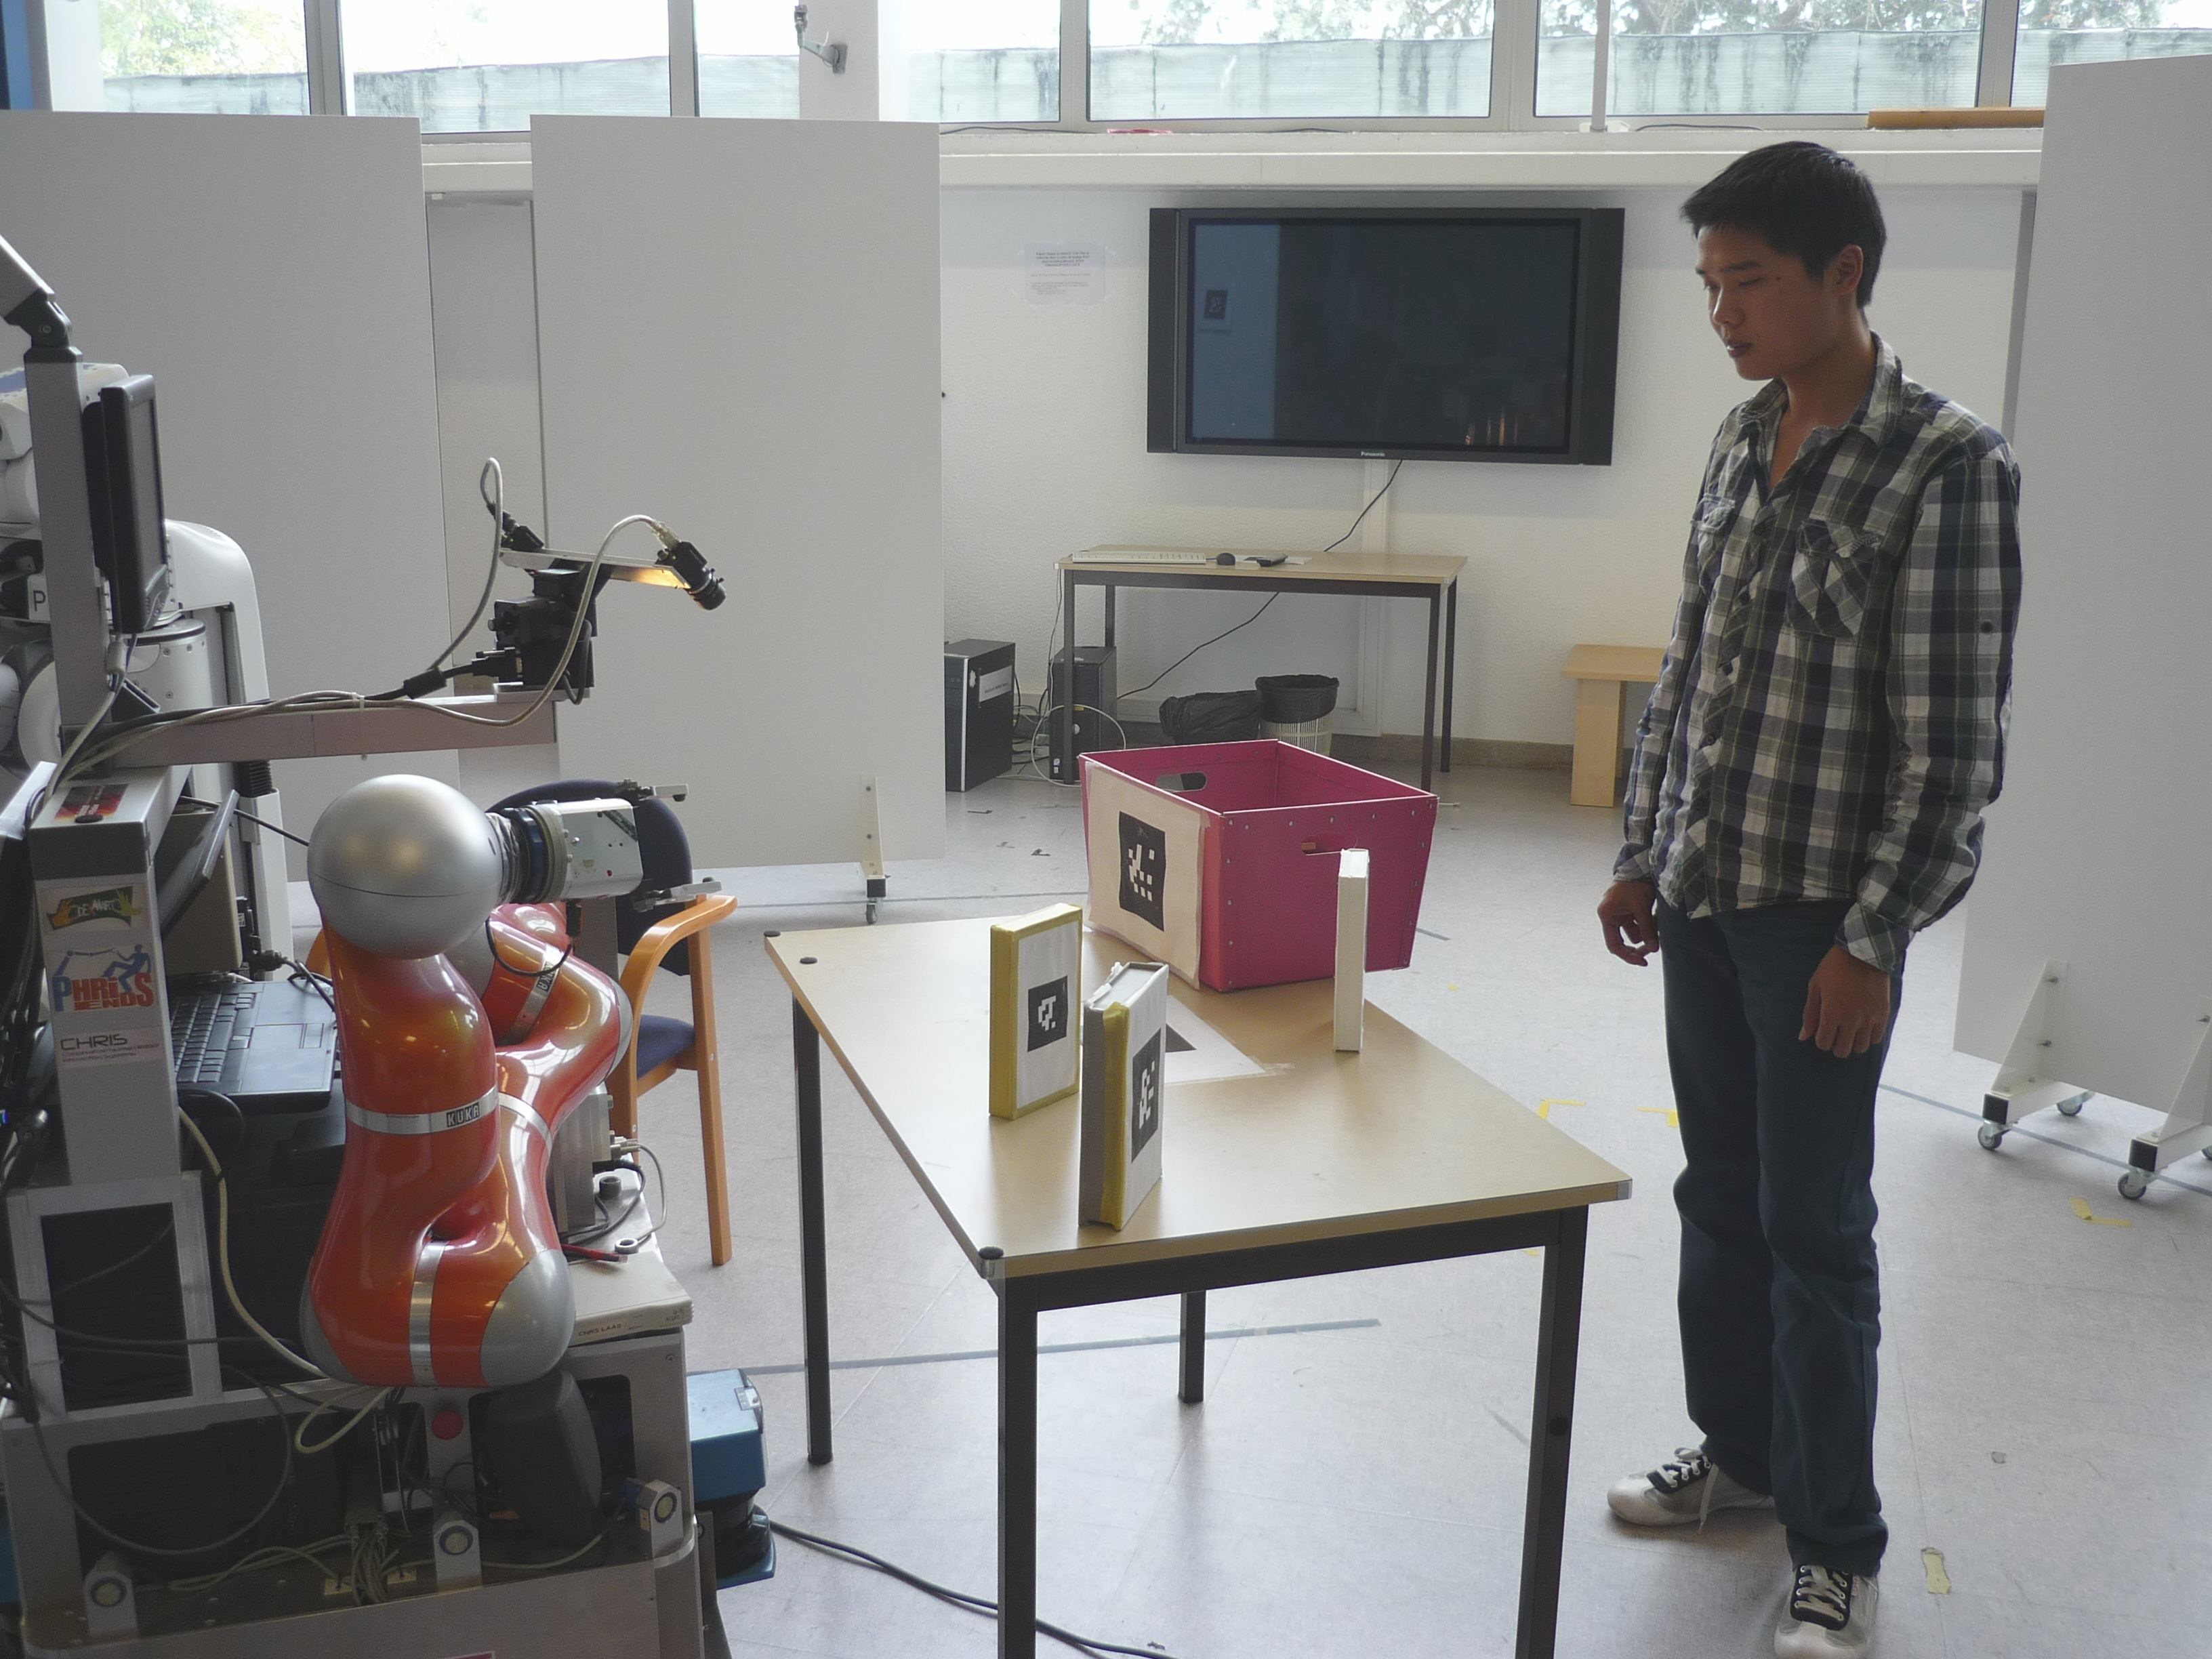
\includegraphics[width=0.5\textwidth]{./figs/etat2-P1010769_brightened-v2.jpg}
       }%
       \subfigure[3d model view of initial state]{%
%          \label{fig:sparkScreenshot}
          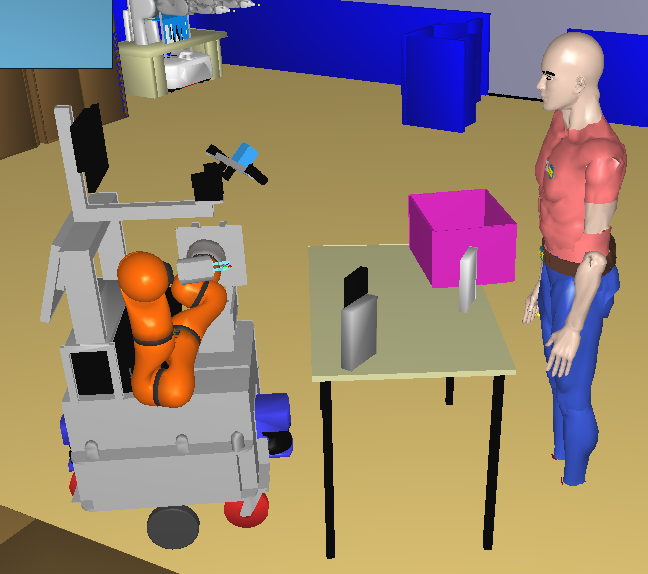
\includegraphics[width=0.43\textwidth]{./figs/etat2_photo.png}
       }\\ %  ------- End of the first row ----------------------%
%
   \end{center}

   \caption{%
     In this situation, there are three tapes on the table. Two tapes
     are only reachable by the robot: the LOTR\_TAPE (black in the 3d
     model) and GREY\_TAPE. The third tape WALLE\_TAPE (white in the
     3d model) and the trashbin PINK\_TRASHBIN are only reachable by
     the human HUMAN1. All tapes are on the table TABLE.  }%

\end{figure}

The set of facts computed in the situation depicted by
Figure~\ref{fig:sparkSubfigures} is the following:
\begin{footnotesize}
%\begin{small}
\begin{verbatim}
                ROBOT                          HUMAN1
PINK_TRASHBIN isReachable false    PINK_TRASHBIN isReachable true 
WALLE_TAPE isReachable false       WALLE_TAPE isVisible true 
LOTR_TAPE isReachable true         LOTR_TAPE isReachable false 
GREY_TAPE isReachable true         GREY_TAPE isReachable false
WALLE_TAPE isVisible true          WALLE_TAPE isReachable true 
LOTR_TAPE isVisible true           LOTR_TAPE isVisible true 
GREY_TAPE isVisible true           GREY_TAPE isVisible true 
WALLE_TAPE isOn TABLE              WALLE_TAPE isOn TABLE 
LOTR_TAPE isOn TABLE               LOTR_TAPE isOn TABLE 
GREY_TAPE isOn TABLE               GREY_TAPE isOn TABLE 
\end{verbatim}
%\end{small}
\end{footnotesize}

%\newline\newline
%\subsubsection*{Hypotheses on objects states and positions}
\vspace{0.3cm}
\noindent
\textbf{Hypotheses on objects states and positions:}
It is sometimes difficult or even impossible to see and/or track an
object in certain states. This happens, for instance, when the object
has been put in a container, when it is in the robot gripper or in the
human hand, and more generally in any state in which it is hidden by
something else. Our robot has a model of the possible symbolic states
for an object (whether the object is on a furniture, in an agent hand,
in a container, etc.).  According to the robot perception of what has
happened since the object was last seen, the robot tries to maintain a
belief of the current possible symbolic states and their associated
probabilities for this object. Such information can be used to update
the beliefs using input from exploration, dialog, human visual
focus,\ldots
SPARK currently provides a simple implementation of such a functionality. The
only managed hypotheses are \emph{in container} and \emph{in agent hand}. We
can have only one hypothesis at the same time. Hypothesis validity is checked
geometrically in case of incoming perception values.


%\subsubsection*{Primitive action recognition}
\vspace{0.3cm}
\noindent {\bf Primitive action recognition:} 
Monitoring human activity is crucial to maintain a coherent state of
the world. Full human action and activity monitoring is a difficult
task that requires knowledge and reasoning both on high level facts
like goals, intentions and plans, as well as bottom-up data from agent
and object motions. Simple temporal and geometric reasoning on human
hand trajectories and potential objects placements can provide some
useful clues for high level human monitoring processes. We call this
temporal and geometric reasoning \emph{primitive action recognition}.

For example, a \emph{pick}, a \emph{throw} or a \emph{place} action
can be recognized by observing that an object on table and an empty
human hand are close to each other, or that the human hand holding an
object is close to a container, etc. Human hand position is either
directly perceived or inferred from its initial perceived trajectory.
We have a simple implementation of such a primitive action recognition
in SPARK that relies on monitoring human hand and its motion near
objects or above containers.

\subsection{Symbolic facts and beliefs management}

The facts produced by the geometric and temporal reasoning component
are stored in a central symbolic knowledge base, called ORO. Besides
acting as a facts database, the ORO platform~\cite{Lemaignan2010}
exposes several functions: operations on knowledge statements relying
on inference (through a continuous first-order logic classification
process), management of \emph{per-agent} symbolic models, and also
higher cognitive and human-robot interaction related functionalities
like categorization of sets of concepts, profiles of memory (that
enable the robot to ``forget'' about some facts), natural language
grounding~\cite{Lemaignan2011}\ldots.

ORO stores independent knowledge models (in our implementation, as
\emph{ontologies}) for each agent (the robot and the humans it
interacts with). The robot architecture components (like the executive
layer or the situation assessment component) can then store the
agents' beliefs in specific models.  Each of these models is
independent and logically consistent, enabling reasoning on different
perspectives of the world that would otherwise be considered as
globally inconsistent (for instance, an object can be visible for the
robot but not for the human. This object can have at the same time the
property \concept{isVisible \textbf{true}} and \concept{isVisible
  \textbf{false}} in two different models). This feature actually
allows us to consider the robot to be endowed with a simple
\emph{theory of mind}~\cite{Scassellati2002}: it can explicitly
model the belief state of its interactors.

ORO also provides an event mechanism that allows components to be
triggered when specific events occur. A component can
for instance subscribe to events of kind \setstmt{?agent isVisible
  true, ?agent type Human}. As soon as the perception layer detects a
human in the robot's field of view and accordingly updates the
knowledge base, the executive layer would be triggered back. The
event framework also takes advantage of the inference capabilities of
ORO. Thus an event can be indirectly triggered if its triggering
conditions can be inferred to be true.

\subsection{Situation Assessment and Context Management Controller} 

Building, updating and maintaining a correct state of the world at
geometric and symbolic level is crucial to the capacity of the robot
to carry on successfully a multi-step interaction with a human. Tight
integration between the robot controller and the geometric and
temporal reasoning functions in SPARK and symbolic facts and beliefs
management in ORO is central.
 
The robot controller has access to the symbolic facts in ORO that are
automatically updated whenever object and agent positions are changed.
Robot controller can also access geometric perceived or inferred
positions of objects and geometric positions and postures of the human
that will be used to orient its cameras.  Building and updating the
state of the world first relies on perceiving objects. Robot
controller can use:

\begin {itemize}
\item Exploration policies: robot will exhaustively scan the table to
  see all what can be seen.

\item Search policies: robot will search an object until it is
  detected if possible, scanning all the table and looking in human
  hand.

\end {itemize} 

Robot reasons on possible positions for non perceived
objects. These hypotheses could be updated using new input from dialogue, human
action and focus of attention. Currently, we manage at most one hypothesis per
object. This hypothesis is produced by robot controller through an inference on
robot or human action. In case of perception conflicts with low probability for
the current hypothesis, robot controller will break this hypothesis and delete
corresponding symbolic fact in the ontology.

Robot must reacts to change in the world not linked to robot
action to drive world update. Robot controller uses SPARK to monitor human hand
motion and primitive action recognition for \emph{pick} and \emph{throw}. As
mentioned above these primitive action recognition should be used with higher
level information on goals, intentions and plans and some exploration to
achieve complex human action and activity monitoring.  In the current
implementation, these primitive actions are over-optimistically interpreted as
the corresponding actions \emph{pick} object and \emph{throw} object.

\subsection{Geometric Reasoning for Situation Assessment}
\label{spark}

\fxfatal{Merge with previous sections}

Anchoring perceptions in a symbolic model requires perception abilities
and their symbolic interpretation. In this section we present
SPARK (\emph{SPAtial Reasoning \& Knowledge}~\cite{Sisbot2011}), a situation assessment reasoner
that generates relevant symbolic information from the geometry of the
environment with respect to relations between objects, robots and humans.
Moreover, the notion of \emph{Perspective
Taking}~\cite{Flavell1992,Tversky1999} is employed at the heart of the
reasoner to provide the robot with the ability to put itself at the human's
place and to reason about the world from different perspectives.

As mentioned in the introduction, this paper does not focus on the sensor-level
perception. We rather assume that the perception of the humans and the objects
is provided as a list of unique identifiers with associated 3D meshes and 6DOF
poses.

\subsection{Capabilities}

There are a number of common properties for a robot and a human related to
their capabilities in a given situation: they can both reach, grasp, look at,
point at, etc. In our context, we group robots and humans into a single category.
Thus, we define agents as entities that can act in the environment and
manipulate it. In this work we focus on the following capabilities from each
agent's perspective\footnote{Note that each of the capabilities described are
computed from each agent point of view, and therefore, also stored in different
models in ORO for further use at the decisional level.}:

\begin{itemize}

\item \emph{Sees}: An important ability to know about an agent is to predict
``what it can see'', \ie what is within its field of view (FOV). A robot being
able to compute this information can then act accordingly. An example
would be a clarification scenario where the human is searching for an object
and the robot is able to infer that he/she is looking for the one that is not
visible (otherwise the user would not be searching for it).
In Figure~\ref{fig::sparkRepresentations}\emph{a} the field of view of a person is illustrated with a
grey cone (broader one). While he is able to see the two small boxes on the
table in front of him, the big box on his right is out of his FOV, and
therefore, he is not able to see it. 

\item \emph{Looks At}: this relation corresponds to what the agent is focused
on, \ie where its focus of attention is directed. This model is based on a
narrower field of view, the field of attention (FOA). 
Figure~\ref{fig::sparkRepresentations}\emph{a}
shows the field of attention of a person with a green cone (narrower one). In
this example only the grey box satisfies the \concept{looksAt} relation.

%\begin{figure}%[!t] 
%\centering
%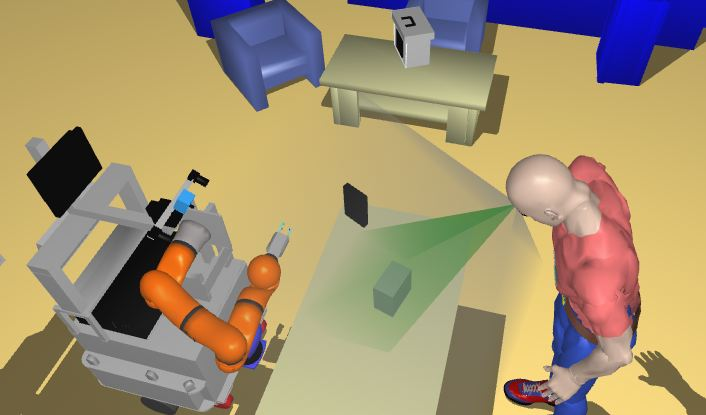
\includegraphics[width=0.8\columnwidth]{figs/looks.jpg} \caption{Representation
%of the field of view (FOV) and the field of attention (FOA) of the human.}
%\label{fig::vis} 
%\end{figure}

\item \emph{Points At}: verifies whether an object is pointed at by an agent.
This relation is particularly useful during interaction when one of the agents
is referring to an object saying ``this" or ``that" while pointing at it.
Section~\ref{disamb-gestures} describes in more detail the combination of both
sources of information (verbal and non-verbal).
 
If a big object occludes a smaller one, and an agent is pointing at them, the
outcome of the evaluation will result only in one relation, \ie \stmt{agent\_01
pointsAt object\_01} since the small one is not visible to the agent.  On the
contrary, if the small object is in front of the big one, then both objects
will satisfy the relation, which may generate an ambiguity (which object the
agent refers to?) that should be solved through higher level reasoning (\eg
context analysis or clarification through verbal interaction).

\item \emph{Reachable}: it allows the robot to estimate the agent's capability
to reach an object, which is fundamental for task planning. For example, if the
user asks the robot to give him/her an object, the robot must compute a transfer
point where the user is able to get the object afterward. 
Figure~\ref{fig::sparkRepresentations}\emph{b} shows different reachability postures for each object
on the table. In the example, the bottle and the box are both reachable for the
human, but the teddy bear is too far. Instead, from the robot's perspective,
the teddy bear is reachable for it, while the bottle is not.

%\begin{figure}%[!t] 
%	\centering
%	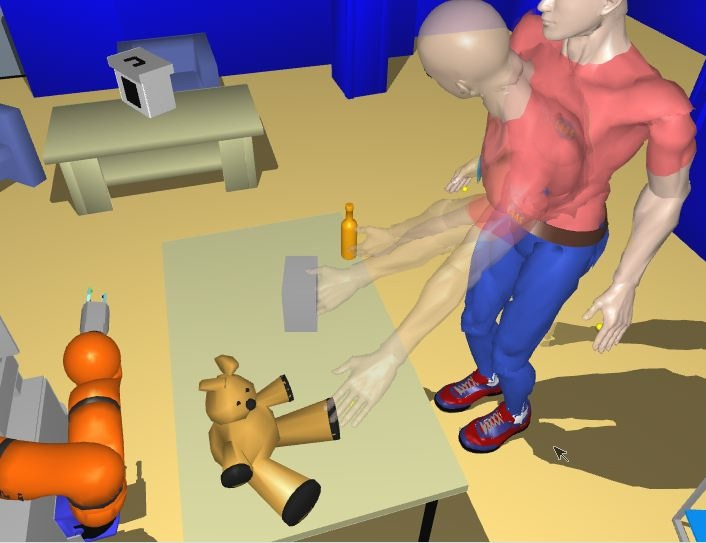
\includegraphics[width=0.8\columnwidth]{figs/reach.jpg} 
%	\caption{Different reaching postures for the human: the bottle and the 
%	box are reachable, while the teddy bear is not.} 
%	\label{fig::reach} 
%\end{figure} 

\end{itemize}

\begin{figure*}[!t]
	\subfigure[]
	{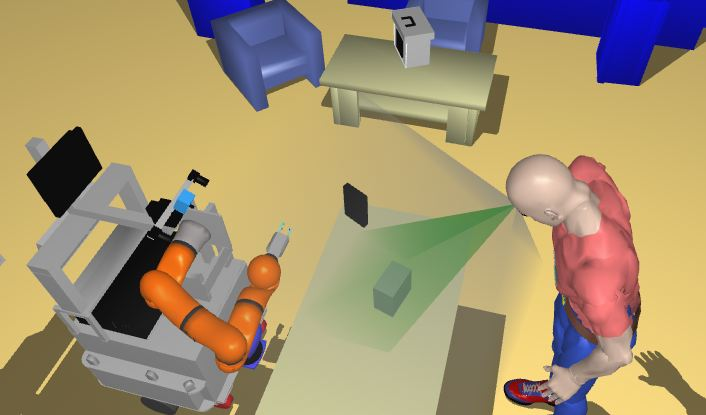
\includegraphics[width=0.35\linewidth]{figs/looks.jpg} \label{(a)}} \quad
	\subfigure[]
	{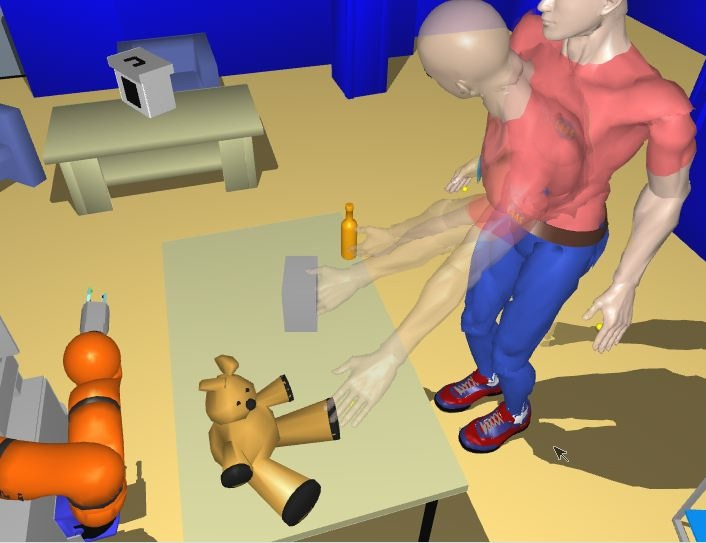
\includegraphics[width=0.3\linewidth]{figs/reach.jpg} \label{(b)}}\qquad	
	\subfigure[]
	{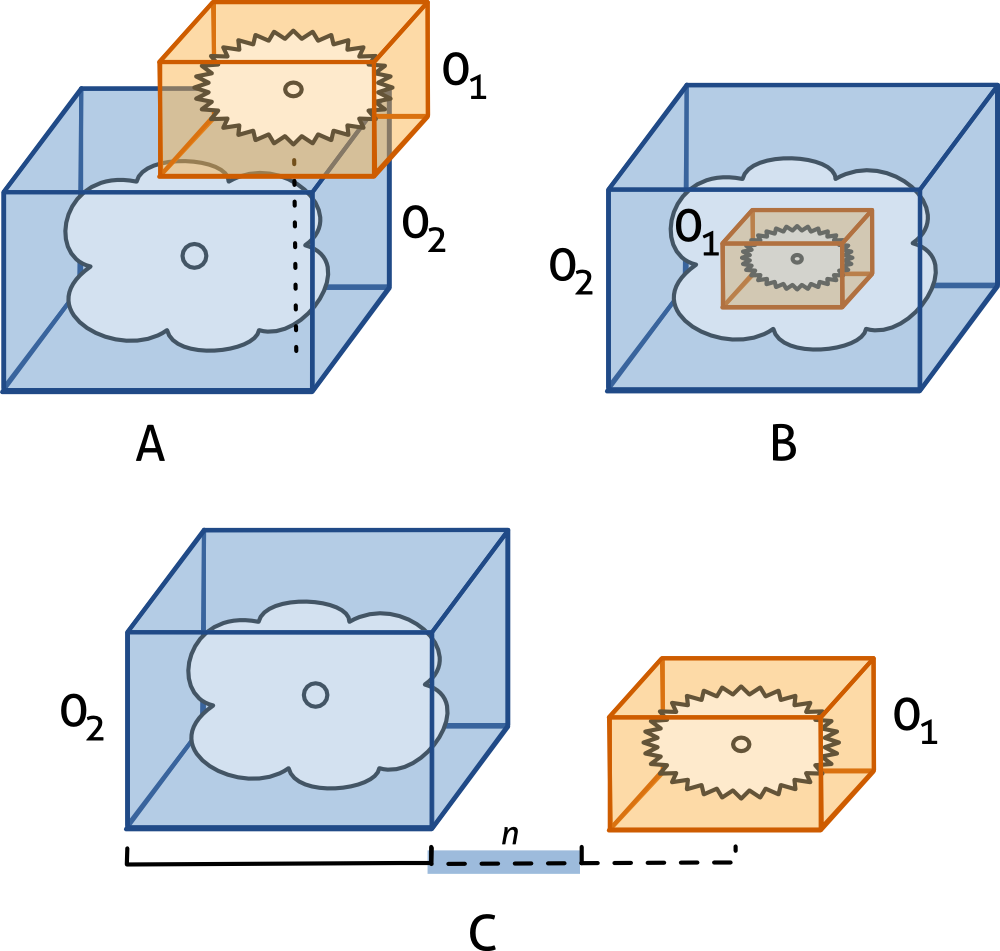
\includegraphics[width=0.25\linewidth]{figs/spatial_relation.png} \label{(c)}} 
	
	\caption{(a) Field of view (FOV) and the field of attention (FOA) of the human. (b) Different reaching postures for the human. (c) Spatial relations between two objects: A) \concept{isOn} relation, B) \concept{isIn} relation, and C) \concept{isNextTo} relation.}
	\label{fig::sparkRepresentations}
\end{figure*} 


While the first three relations (\concept{sees}, \concept{looksAt} and
\concept{pointsAt}) are computed through a model based approach, the latter one
is based on the Generalized Inverse Kinematics with pseudo inverse
method~\cite{Nakamura90,Baerlocher04} to find a collision free posture for the
agent where its end-effector is at the center of the object within a given
tolerance. The details of these computations are out of the scope of this
article.

\subsection{Locations}

One way of referring to object's positions is based on human's symbolic 
descriptors, instead of using their precise position. In fact, in many cases, 
this information is the most precise information available since humans do not 
store the numeric coordinates of objects. These type of descriptors have been 
studied in the context of language grounding 
(\cite{O'Keefe1999,Matuszek2010,Regier2001,Kelleher2009,Blisard2005}). In this 
work we focus on the following relations which are computed with respect to the 
position of the agents and the objects:

\begin{itemize} 

\item \emph{Location according to an agent}: The predicate
\concept{isLocatedAt} represents spatial locations between agents and objects.
For example we say ``it is on my right, on your left, ...'' We compute these
spatial locations by dividing the space around the referent (an agent) into $n$
regions based on arbitrary angle values relative to the referent orientation.
For example, for $n = 4$ we would have the space divided into \emph{front,
left, right} and \emph{back}. Additionally, two proximity values, \emph{near}
and \emph{far}, may also be considered. The number of regions and proximity
values can be chosen depending on the context where the interaction takes
place.

\item \emph{Location according to an object}: We can also refer to object
locations with respect to other objects in the environment, such as \emph{above,
next to, in}, etc. In this work we compute three main relations based on the
bounding box and center of mass of the objects 
(Figure~\ref{fig::sparkRepresentations}\emph{c}): 

\begin{itemize}
	\item \concept{isOn}: computes if an object $O_1$ is on another object $O_2$ by
	evaluating the center of mass of $O_1$ according to the bounding box of $O_2$.

	\item \concept{isIn}: evaluates if an object $O_1$ is inside another object
	$O_2$ based on their bounding boxes $BB_{O_1}$ and $BB_{O_2}$.

	\item \concept{isNextTo}: indicates whether an object $O_1$ is next to another
	object $O_2$. We cannot use a simple distance threshold to determine if two
	objects are next to each other since the relation is highly dependent on the
	dimensions of the objects. For instance, the maximum distance between large
	objects (\eg two houses) to consider them as being next to each other is much
	larger than the maximum distance we would consider for two small objects (\eg
	two bottles). Thus, the relation between the dimensions and the distances of
	the objects are taken into account.  

%\begin{figure} 
%	\centering
%	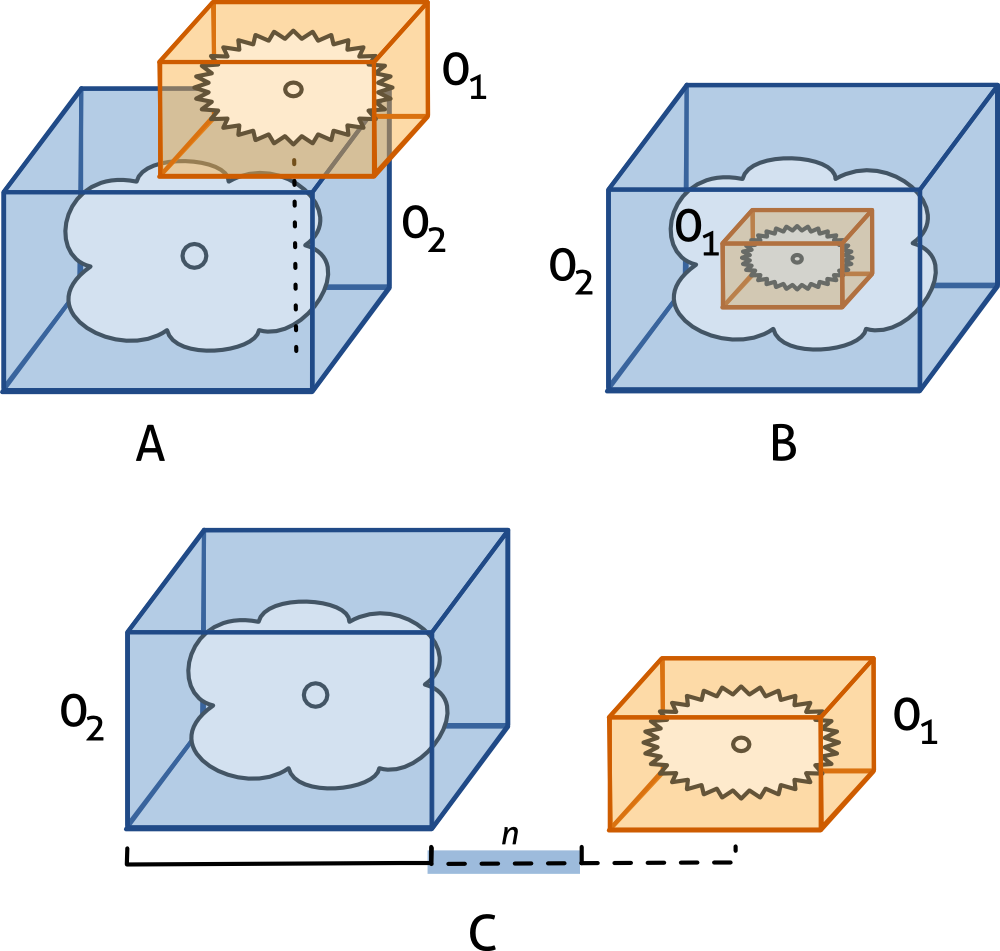
\includegraphics[width=0.6\columnwidth]{figs/spatial_relation.png}
%	\caption{Spatial relations between two objects: A) \concept{isOn} relation, 
%	B) \concept{isIn} relation, and C) \concept{isNextTo} relation.} 
%	\label{fig::sprelation} 
%\end{figure}

\end{itemize} 
\end{itemize}

To ensure the different agent models are up-to-date, all these properties are
always computed on-line, each time the current state of the world changes.

SPARK can be compared to the \emph{Grounded Situation Model} (GSM) introduced
by Mavridis and Roy~\cite{Mavridis2005} in the sense that they both provide an
amodal physical representation of the world used as a mediator between the
sensor space and symbolic models. They have however different features: while GSM enables representation of time and imaginary objects (whose
existence is hinted by verbal assertions from a human, also called
\emph{presupposition accomodation}), SPARK offers a richer 3D model that
enables the computation of several spatial relationships between
objects and an effective implementation of perspective taking capabilities.





%%%%%%%%%%%%%%%%%%%%%%%%%%%%%%%%%%%%%%%%%%%%%%%%%%%%%%%%%%%%%%%%%%%%%%%%%%%%
%%%%%%%%%%%%%%%%%%%%%%%%%%%%%%%%%%%%%%%%%%%%%%%%%%%%%%%%%%%%%%%%%%%%%%%%%%%%

\section{Explicit Knowledge Management} \label{cognitivekernel}

\subsection{On Knowledge Representation} \label{knowledge_representation}

While \emph{knowledge} has no general definition that researchers agree on, for
our own purposes we define knowledge as \emph{information interpreted in the
cultural and social context of the robot}, where information is a
\emph{statement} or an \emph{assertion} about the world\footnote{In this paper,
statements are always triples \stmt{subject predicate object}, \ie binary
relations between entities.}. In practical terms, knowledge is made of
statements that are \emph{contextualized}, if possible \emph{synthesized}, and
\emph{limited} to a domain of validity. These three features have important 
consequences for the way a knowledge representation and storage system must 
be designed. Let us examine them:

\paragraph{Contextualizing} is the ability for a cognitive system to connect a
fact with a \emph{cultural context}, an \emph{interpretive scope} and the set
of other facts previously acquired by the agent.
%~ Since machines are limited to syntactic (in contrast to semantic)
%processing, we are mostly looking for a syntactic (\ie, based on symbols)
%matching between concepts representations (in our case, sets of alphanumeric
%characters).\fxfatal{il faut sans doute évoquer ici la relation
%sémantique/syntactique que propose Choamsky}.

We call \textit{cultural context} a broad set of common, general facts that are
considered widely accepted among the interactors (\eg ``bottles may contain
water''). This knowledge is often referred as \emph{common-sense knowledge}.

By \emph{interpretive scope} we mean that a concept may have different
interpretations depending on the agent, the current situation or the time frame
the statement belongs to. Since a fact in one scope can be different (or even
inconsistent) with a fact in another scope (for instance, one object can be
visible for the robot and invisible for another agent), the underlying
knowledge representation system must properly handle these interpretive
frameworks.

Note that the focus of ORO is on enabling such context to be
effectively represented rather than actually identifying the current context.
While several approaches for building contextualized knowledge are proposed in this
paper (symbolic environment interpretation, perspective taking, grounded
natural language resolution, self-awareness of its own activity), much remains
to be done for a robot to actually identify its current context as well as
contexts that may be referred to.

\paragraph{Synthesis} corresponds to the identification of facts and their
components (concepts and predicates) with respect to other facts. For instance,
if the robot observes a human sitting down at a table, and at the same time, we
tell it that ``Peter is sitting at the table'', we would like the robot to
infer that ``Peter'' may be the name of the human. \textit{Synthesis}
refers to the fact that several, \textit{a priori} uncorrelated, facts
must be associated with the same common concept. This process requires the
ability to control the logical consistency of the knowledge corpus. To
continue with the previous example,  if we add the fact that the human that
is sitting is a woman, the synthesis ``Peter is the name of the human'' is
not valid anymore.

\paragraph{Domain of validity} specifies the scope in which
 information is (believed to be) true. It covers several aspects: temporal,
situational and probabilistic. While related to the previous concept of
\emph{interpretive scopes}, the domain of validity addresses the question
whether a fact must be or not considered in a given context. This validity
limitation is not usually carried by the fact itself. In the previous example,
for instance, the robot observes a human sitting at a table.  The fact ``a
human is sitting at the table'' is true only for a limited period of time,
until the human stands up. This period of time is not directly accessible
(the robot does not know how long the human plans to stay), but the
knowledge representation must be able to deal with this uncertainty and
should explicitly label this fact as being limited in time.
%~ ~ To know if a fact is permanent or transitional (as defined by Pollock
%\fxfatal{citation de Langage et Cognition, page 50}) is difficult (especially
%considering that a feature may be considered as permanent or not depending of
%the context: within the situation ``a familly meal''\fxfatal{Check
%translation!}, the fact ``the human is sitting at the table'' could be
%considered as permanent. Conversely, ``ground is static'' is generally
%considered as a static fact, expect if we are talking of planetary mechanics
%for instance. The difficulty lies in the selection of the relevant situation
%in which reasoning must be carried out at a given time) and have currently to
%be defined in the cultural background of the robot.

These three aspects lead us to envisage a knowledge representation system
characterized by the following abilities: 
\begin{itemize}
	\item represent raw information,
	\item render a general cultural background, in the form of common-sense knowledge,
	\item attach interpretive scopes to new statements,
	\item add and connect new statements to knowledge already present,
	\item store restrictions on the domain of validity of the knowledge.
\end{itemize}

Besides, the following active processes would be desirable:
\begin{itemize}
	\item acquire and maintain knowledge perceived from the physical world or
	retrieved from other sources (interaction with other agents, web-based contents,...)
	\item synthesize facts as much as possible,
	\item monitor contexts and accordingly manage the validity of the stored knowledge,
	\item ensure the logical consistency of the knowledge repository, and
	explicit inconsistencies when required\footnote{One may argue that the real world is 
	inherently inconsistent. In this article, we make a
	\textit{consistent world} assumption, in order to leverage reasoning
	capabilities of the first-order logics. This is supported by the natural
	tendency of humans themselves to provide a consistent explanation of their
	world.}.
\end{itemize}

This list does not cover all the possible features that could be exposed by a
symbolic knowledge management system. Bio-inspired memory management (the
ability to forget or reinforce knowledge) or curiosity (the ability to identify
lacking knowledge and actively trigger behaviours to acquire it --Hawes et
al.~\cite{Hawes2011} have contributed in this area with \emph{Dora}, a
robot endowed with motivation mechanisms to explore unknown regions of
the environment--), to give some examples, could arguably be added to the list.
However, this first analysis sets a convenient reference frame to understand
and evaluate knowledge representation systems, including the \textsc{ORO}
knowledge management system we propose.

%\begin{figure}[!ht]
%\centering
%  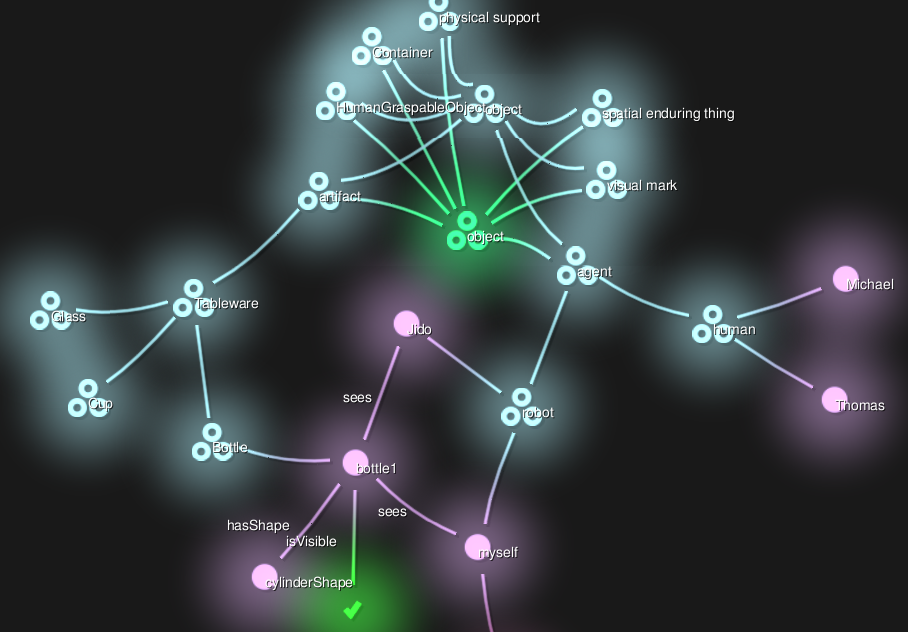
\includegraphics[width=\columnwidth]{figs/snapshot_oroview.png}
%  \caption{Live snapshot from the \emph{oro-view} viewer depicting the
%  knowledge model of the robot during an experiment. Dots represent
%  instances (ABox), while circles pyramids are classes (TBox)}
%  \label{fig|oro-view}
%\end{figure}

\subsection{ORO Architecture}

The ORO platform~\cite{Lemaignan2010} is primarily designed as a central
knowledge storage service implemented as a server where the robot
components can add or query statements at run-time. Figure~\ref{fig|oro-overview}
illustrates the overall architecture. The \emph{front-end} accepts and manages
connections from client components. The clients' requests are processed by a
set of internal modules: basic operations on statements, but also higher
cognitive and human-robot interaction related functionalities are available
(detailed thereafter). External plugins can also be easily added. The modules
rely on several parallel ontology \emph{back-ends} where the knowledge is
actually stored.

Knowledge is represented in ORO in the Description Logics formalism (using the
OWL-DL --\emph{Web Ontology Language - Description Logics}-- language), as
RDF (\emph{Resource Description Framework}) triples (for instance \stmt{robot
isIn kitchen}). We use the Jena\footnote{\url{http://jena.sourceforge.net/}}
framework as the underlying library to load and build an in-memory OWL model. We
use it in conjunction with the
Pellet\footnote{\url{http://clarkparsia.com/pellet/}} reasoner to ensure the
continuous classification of the OWL concept graph: at run-time, newly added
statements are continuously reasoned about (\emph{classified}), and at any time,
the server exposes a complete set of statements, both the asserted ones and the
inferred ones. For instance, if \stmt{socrates type Human} and \stmt{Human
subClassOf Mortal} are asserted, the server transparently adds the inferred
statement \stmt{socrates type Mortal}, and a later query retrieving all mortal
entities would return \concept{socrates} as well. The language of the OWL
family make the \emph{Open World Assumption} (if a fact can not be inferred as
true, it does not mean that it is inferred to be false), and the Pellet
reasoner honors this assumption as well.

\begin{figure}[!t]
\centering
  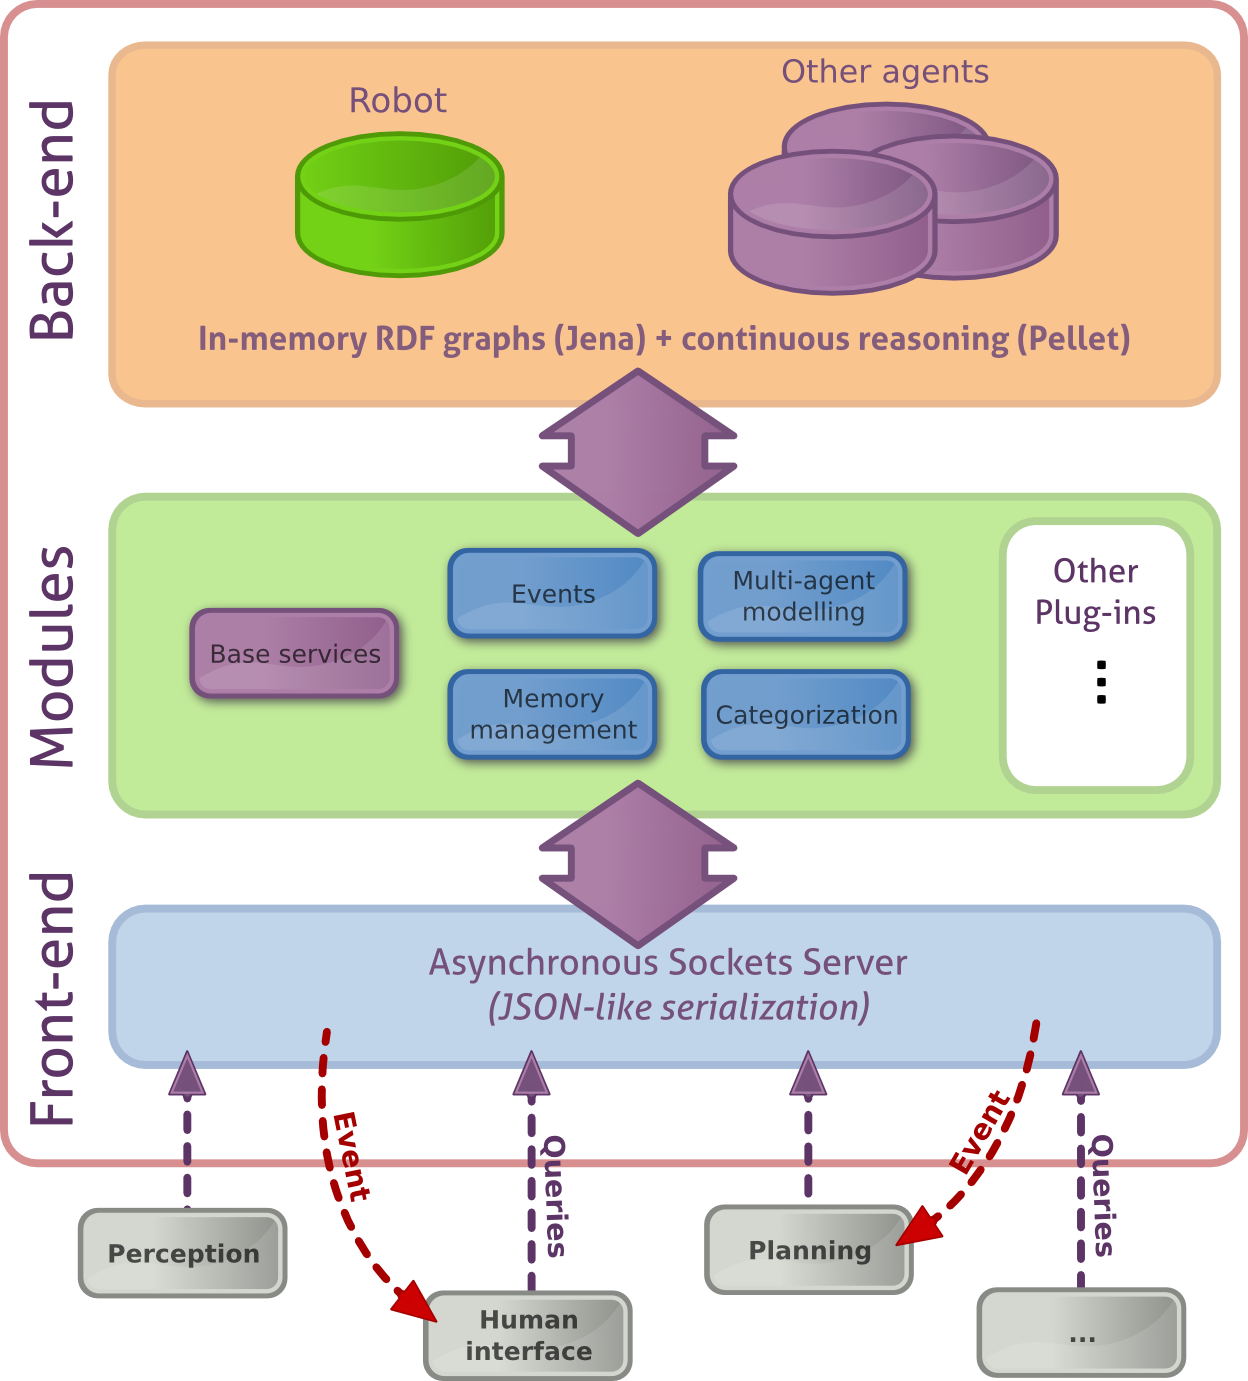
\includegraphics[width=0.8\linewidth]{figs/oro_architecture.png}
  \caption{Overview of the ORO architecture.}
  \label{fig|oro-overview}
\end{figure}

\subsection{The OpenRobots Common-Sense Ontology}
\label{ontology}

The first requirement identified in section~\ref{knowledge_representation}
refers to the modeling of a cultural background, a common-sense knowledge
assumed to be shared by all agents.
The ORO server can be loaded with an initial set of statements which we call
the \emph{OpenRobots Common Sense Ontology}. It defines a small set of concepts
(and implicitly, a vocabulary) that can be used by all the modules of the robot
to unambiguously add or query facts. Moreover, the same ontology declares rules
and logical properties that are later on used for inference.

The \emph{OpenRobots Common Sense Ontology} defines a small set of classes (56
are currently defined) and predicates (60 are currently defined) focused on
concepts useful for human-robot interaction. It includes both very broad
categories like \concept{SpatialThing}, \concept{Event} or \concept{Action},
and much more concrete concepts as \concept{Table}, \concept{Book} or colors.
Available predicates allow us to describe the state of the agents and the world
with relations like \concept{isOn}, \concept{sees},
\concept{currentlyPerforms}, etc.

Several significant projects are trying to provide such a machine-processable
repository of common sense facts produced by humans (the \textsc{OpenMind}
project\footnote{\url{http://www.openmind.org/}}, for instance). These
knowledge bases are valuable but remain difficult to use in a pervasive way
because of both their incompleteness and the lack of good connections with
underlying, unambiguous concepts.
%\cite{Singh2002}

Our common sense ontology is closely aligned with the open-source
OpenCyc\footnote{\url{http://www.opencyc.org}} upper ontology.
OpenCyc defines a large taxonomy of concepts and semantic
relationships between concepts that are used in several other projects
(\textsc{WordNet, DBpedia}). This potentially eases the exchange and addition
of knowledge from these other sources. Moreover, it also enables knowledge
exchange with other robots (for instance, the works previously mentioned by
Daoutis and Tenorth rely on the same Cyc concepts).

\subsection{Reasoning and Dynamic Knowledge Structuring}

As previously mentioned, ontologies in ORO are written in OWL. The
Pellet reasoner supports most of the OWL constructs and allows several types of
reasoning:

\begin{itemize}
	\item inheritance
	\item property axioms
		\begin{itemize}
		\item entailments based on predicates' domain and range,
		\item cardinality constraints (including \concept{allValue}, 
		\concept{someValue}, \concept{hasValue}),
		\item property characteristics (symmetry, transitivity)
		\end{itemize}
	\item class restrictions like: \par \footnotesize \concept{Bottle} $\equiv$
		\concept{Artifact} {\bf that} (\concept{hasShape} {\bf value}
		\concept{cylinderShape})\footnote{This example uses the \emph{Manchester
		syntax}, \url{http://www.w3.org/TR/owl2-manchester-syntax/}} \normalsize
	\item set operations like: \par \footnotesize \concept{Color} $\equiv$ {\bf unionOf}(\concept{blue},
		\concept{green}, \concept{orange}, \concept{black}...) \normalsize
	\item generic SWRL ({\em Semantic Web Rule Language}) rules like: \par
		\footnotesize \concept{looksAt(?agt, ?obj)} $\land$
		\concept{pointsAt(?agt,?obj)} \par $\Rightarrow$ \concept{focusesOn(?agt, ?obj)}
		\normalsize 
	\end{itemize}

We provide in ORO accessors to query, add or remove all these properties and
restrictions (except the SWRL rules) at run-time. This allows
knowledge introspection and enables the robot to alter its own knowledge
structures (the so-called \emph{T-Box} model) during its life-time by adding
new constraints and properties to classes and predicates.
The \emph{Naming} experiment (section~\ref{naming}) gives a simple example of
such knowledge restructuring.

\subsection{ORO Features}
\label{features}

Besides storing and reasoning about knowledge, we have developed in ORO several
features to manage knowledge at higher level: 
%independent cognitive models for
%each agent the robot interacts with, categorization capabilities, different
%profiles of memory and events registration.

\subsubsection{Base Functionalities}
\label{base}

ORO offers an extended set of methods to process facts at the triples level,
including:
\begin{itemize}
	\item statement (\ie RDF triples) insertion, removal, update,

	\item pattern-based statements removal,

	\item pattern-based queries (for instance, \stmt{ * isOn
	table}, which means ``return me all objects on table'') and filters (for
	instance, \concept{weight < 150.0}),

	\item consistency check, insertion of statements with consistency
	constraint (only if the new fact does not lead to inconsistencies),
	
	\item fast concept lookup, with possible multi-lingual support (through the
	\concept{@lang} XML annotation, labels of concept can be translated, and
	specific translations can be queried for),

	\item standard SPARQL queries.

\end{itemize}

While these basic functionalities enable the incremental construction (and
exploitation) of a consistent knowledge model, the \emph{Common Sense Ontology}
helps build assertions that are related to previous ones by offering
a predefined vocabulary.

\subsubsection{Representation of Alternative Cognitive Models}
\label{alterite}

As pictured in Figure~\ref{fig|oro-overview}, ORO stores independent cognitive
models for each agent it interacts with. When ORO actually identifies a new
agent (or infers that some instance is an agent), it automatically creates a
new, separate, in-memory OWL model for that agent. Thus, different robot
components, like supervision or situation assessment, may then store the
agents' beliefs in separate models. All knowledge processing functions in the
robot's primary model are equally available in every agent's model, which
allows us to store and reason on different (and possibly globally inconsistent)
models of the world.

Each of these models is independent and logically consistent,
enabling reasoning on different perspectives of the world that would otherwise
be considered as globally inconsistent (for instance, an object can be visible for the
robot but not for the human. This object can have at the same time the property
\concept{isVisible \textbf{true}} and \concept{isVisible \textbf{false}} in
two different models). 

This feature actually allows us to consider the robot to be endowed with a
\emph{theory of mind}~\cite{Scassellati2002}: the robot can explicitly model
the belief state of its interactors, opening new possibilities for the control
architecture. In section~\ref{exp:disambVPT} we present an example of how we use this feature to
make sense of user sentences from his/her point of view. Moreover,
these multiple models can be viewed as different interpretive scopes,
allowing the robot to interpret the same reality from different points of view.

\subsubsection{Categorization}
\label{categorization}

We have implemented several algorithms (common ancestors, computation of the
best discriminant~\cite{Ros2010b}) to help the robot cluster a set of
concepts based on their symbolic similarities. One particular application of these functions is discrimination.
While interacting with a user, the robot quite often needs to clarify an
ambiguity produced by its human partner. For instance, a user may refer to a
``bottle'' where two bottles are currently visible. Discrimination routines
can identify possible (symbolic) differences (\eg the color or the size of the
bottles) that permit the robot to ask an accurate question to the user in order
to solve the ambiguity. This discrimination can occur from the robot's
perspective or from a specific agent's perspective. Usage of these
categorization abilities are illustrated in Sections~\ref{dialogs:disamb} and~\ref{spygame}.

\subsubsection{Memory Profiles}
\label{memory}

We have designed a simplified bio-inspired memory model to store
statements in different \emph{memory profiles}. These include \emph{short term
memory} and \emph{long term memory}. Each profile is characterized with a
lifetime, which is assigned to the stored facts. When the lifetime of a fact
expires, ORO automatically removes it.

\subsubsection{The Events Framework} 
\label{events} 

Lastly, ORO allows external modules to be triggered when specific events occur.
For instance, when a logical sentence becomes true or false, or if a new
instance of a certain class is added. One immediate application is reactive
supervision: a component could for instance subscribe to events of kind
\setstmt{?agent isVisible true, ?agent type Human}. As soon as the perception
layer detects a human in the robot's field of view and accordingly updates the
knowledge base, the supervision component would be triggered back. The event
framework also takes advantage of the inference capabilities of ORO. Thus an
event can be indirectly triggered if its triggering conditions can be inferred
to be true.

The next sections describe how symbolic knowledge is actually produced and added to
ORO.




%%%%%%%%%%%%%%%%%%%%%%%%%%%%%%%%%%%%%%%%%%%%%%%%%%%%%%%%%%%%%%%%%%%%%%%%%%%%
%%%%%%%%%%%%%%%%%%%%%%%%%%%%%%%%%%%%%%%%%%%%%%%%%%%%%%%%%%%%%%%%%%%%%%%%%%%%

\section{First Application: Goal and Plan Management}
\label{sec:plan}

\fxfatal[author=Severin]{Reformulate this section to put emphasis on 'How we
use the whole architecture to make symbolic planning grounded into the real
physical world.'}

The Goal and Plan Management activity involves the human-aware
symbolic task planner component and the dedicated robot controller
activity (Figure~\ref{architecture_fg}).

\subsection{Symbolic Task Planning}

In order to devise how a given goal can be accomplished, the robot has
to elaborate a plan,~\textit{i.e.} a set of actions to be achieved by
the robot and its human partners.  This is the role of a HATP
\cite{Alili2008} (for Human Aware Task Planner).  HATP is based on a
Hierarchical Task Network (HTN) refinement which performs an iterative
task decomposition into sub-tasks until reaching atomic
actions~\cite{Nau2003}.  The planning domain defines a set of methods
describing how to decompose a task and can be seen as the Howto
knowledge of the robot.  HATP is able to produce plans for the robot's
actions as well as for the other participants (humans or robots). It
can be tuned by setting up different costs depending on the actions to
apply and by taking into account a set of constraints called social
rules. This tuning aims at adapting the robot's behavior according to
the desired level of cooperation of the robot.

%\subsubsection*{Agents and action streams:}
\vspace{0.3cm}
\noindent
\textbf{Agents and action streams:}
The robot plans not only for itself but also for the other agents. The
resulting plan, called ``shared plan'' is a set of actions that form
a stream for each agent involved in the goal achievement. Depending on
the context, some ``shared plans'' contain causal relations between
agents. For example, the second agent needs to wait for the success of
the first agent's action to be able to start its own action. When the
plan is performed, causal links induce synchronization between
agents. Figure~\ref{plan_hatp1} illustrates a plan with two streams.

\begin{figure}[htbp]
  \centering
  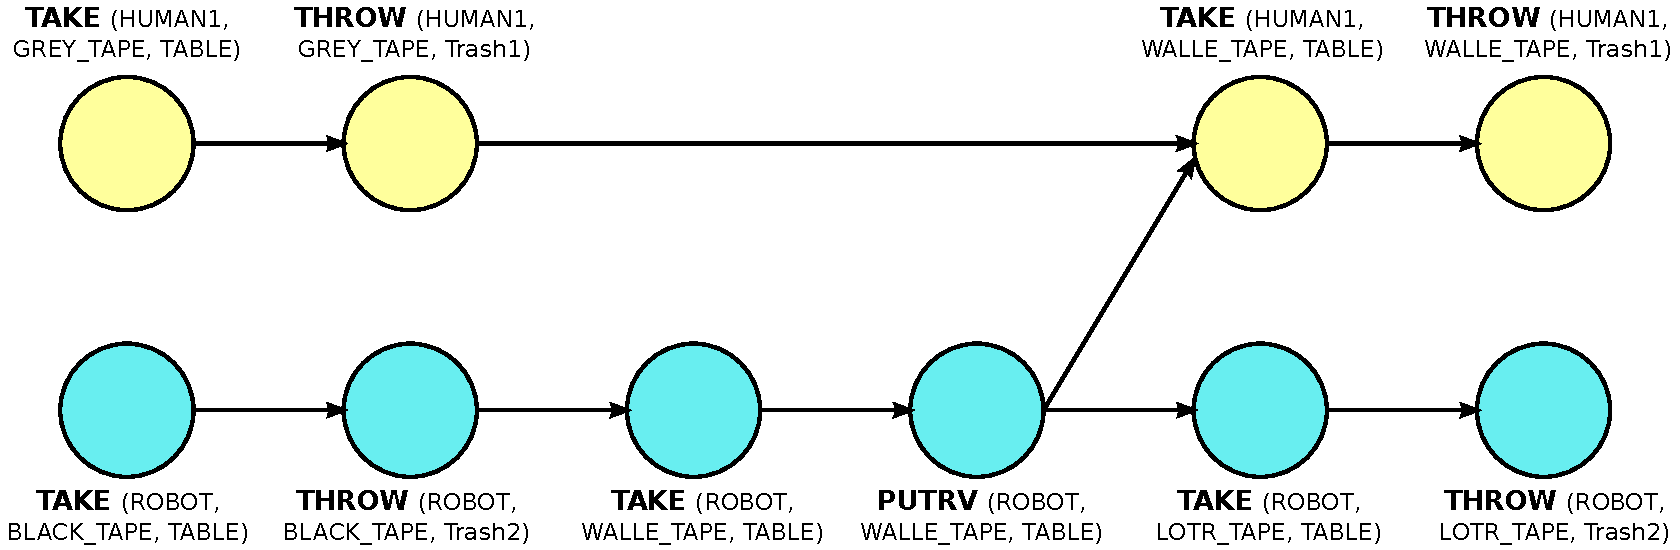
\includegraphics[width=0.95\columnwidth]{./figs/first_plan.pdf}
  \caption{A plan produced by HATP with 2 streams}
  \label{plan_hatp1}
\end{figure}

%\subsubsection*{Action costs and social rules:}
\vspace{0.3cm}
\noindent
\textbf{Action costs and social rules:}
A cost and a duration function is associated to each action.
The duration function provides a duration interval for the action
achievement and is used, in one hand, to schedule the different
streams and, in the other hand, as an additional cost function.
In addition to these costs, HATP also takes into account a set of social
rules.  Social rules are constraints aiming at leading the plan
construction towards the best plan according to some human
preferences. The social rules we have defined so far deal with:

\begin{itemize}
\item undesirable state: to avoid a state in which the human could
  feel uncomfortable;
\item undesirable sequence: to eliminate sequences of actions that can
  be misinterpreted by the human;
\item effort balancing: to adjust the work effort of the agents;
\item wasted time: used to avoid long delays between the actions of
  the human partner;
\item intricate links: to limit dependencies between the actions of
  two or more agents.
\end{itemize}

\begin{figure}[htbp]
  \centering
  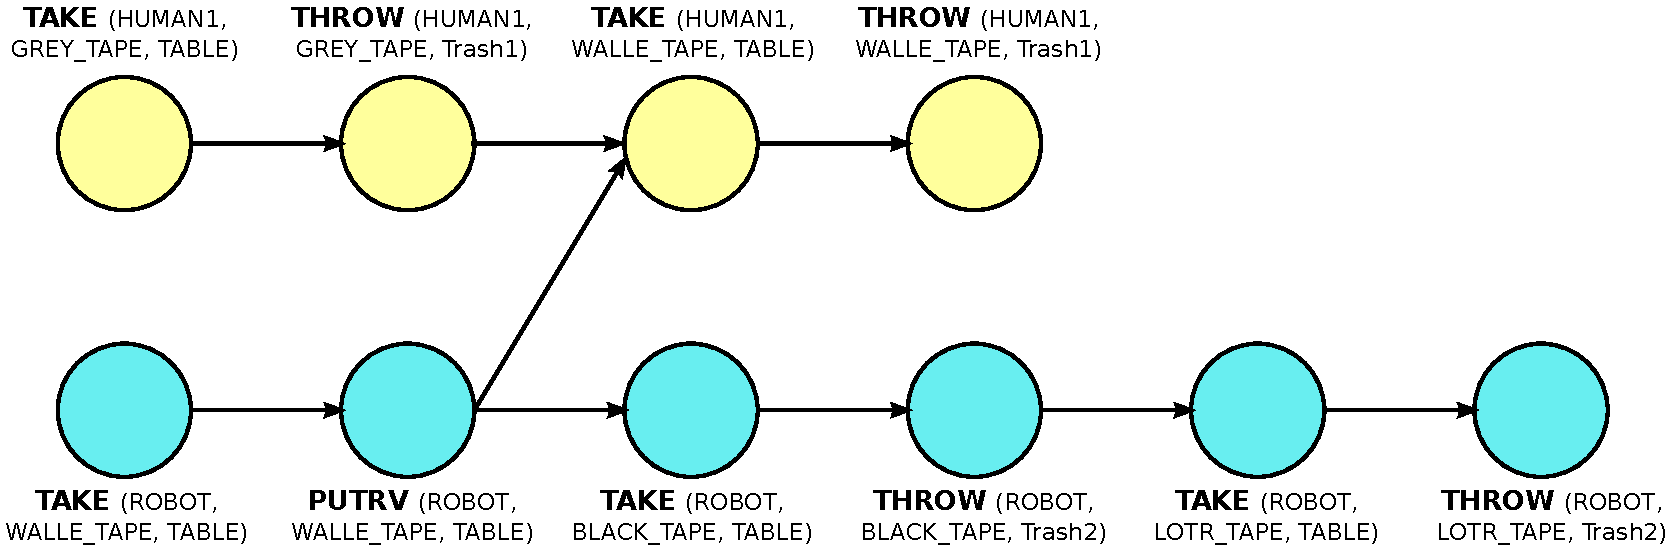
\includegraphics[width=0.95\columnwidth]{./figs/second_plan.pdf}
  \caption{A plan with the wasted time social rule}
  \label{plan_hatp2}
\end{figure}

Figure~\ref{plan_hatp2} illustrates an alternative plan to the previous 
one (Figure~\ref{plan_hatp1}) if the wasted time social rule is used.
The obtained shared plan is the best plan according to a global evaluation of
these multiple criteria.

%\subsubsection*{Several levels of cooperation:} 
\vspace{0.3cm}
\noindent
\textbf{Several levels of cooperation:} 
By tuning its costs
and adapting its social rules, HATP can be used to compute various
alternative plans. These plans can be categorized into several levels
of cooperation

\begin{itemize}
\item helping the human to achieve his goal by acting for him
\item sharing concrete resources by handing some objects
\item collaboration of the robot and the human by coordinating their
  actions towards a human-robot joint goal.
\end{itemize}

\subsection{ Goal and plan Controller}
Figure~\ref{goal_plans_fg} sums up the Goal and Plan Management as
implemented in the robot controller.  When an event announcing a new
goal is caught by the controller, the validity of this goal is tested:
does it corresponds to capabilities of agents? is it not already
achieved? Then, the goal is sent to HATP which produces a first plan.
A goal is considered achievable as long as the planner computes a
valid plan and it is not abandoned by the human.

Plan execution consists in the management of all the actions of the
plan. Human and robot are not acting both at the same time.  In case
of plan failure a new plan is requested and executed.

The management at the action level is done in three steps. First, the
action preconditions are tested over the current state of the
world. Then the action is executed and monitored (only monitored of it
corresponds to a human action).  Finally, the expected effects are
verified in order to acknowledge the action achievement.

Concerning the speech acts during plan management, the robot informs
its partners on the goal existence and status, plan existence and
status, ongoing plan action, plan action failure, failing facts for
action precondition or effect assessment.

\begin{figure}[thpb]
  \centering
  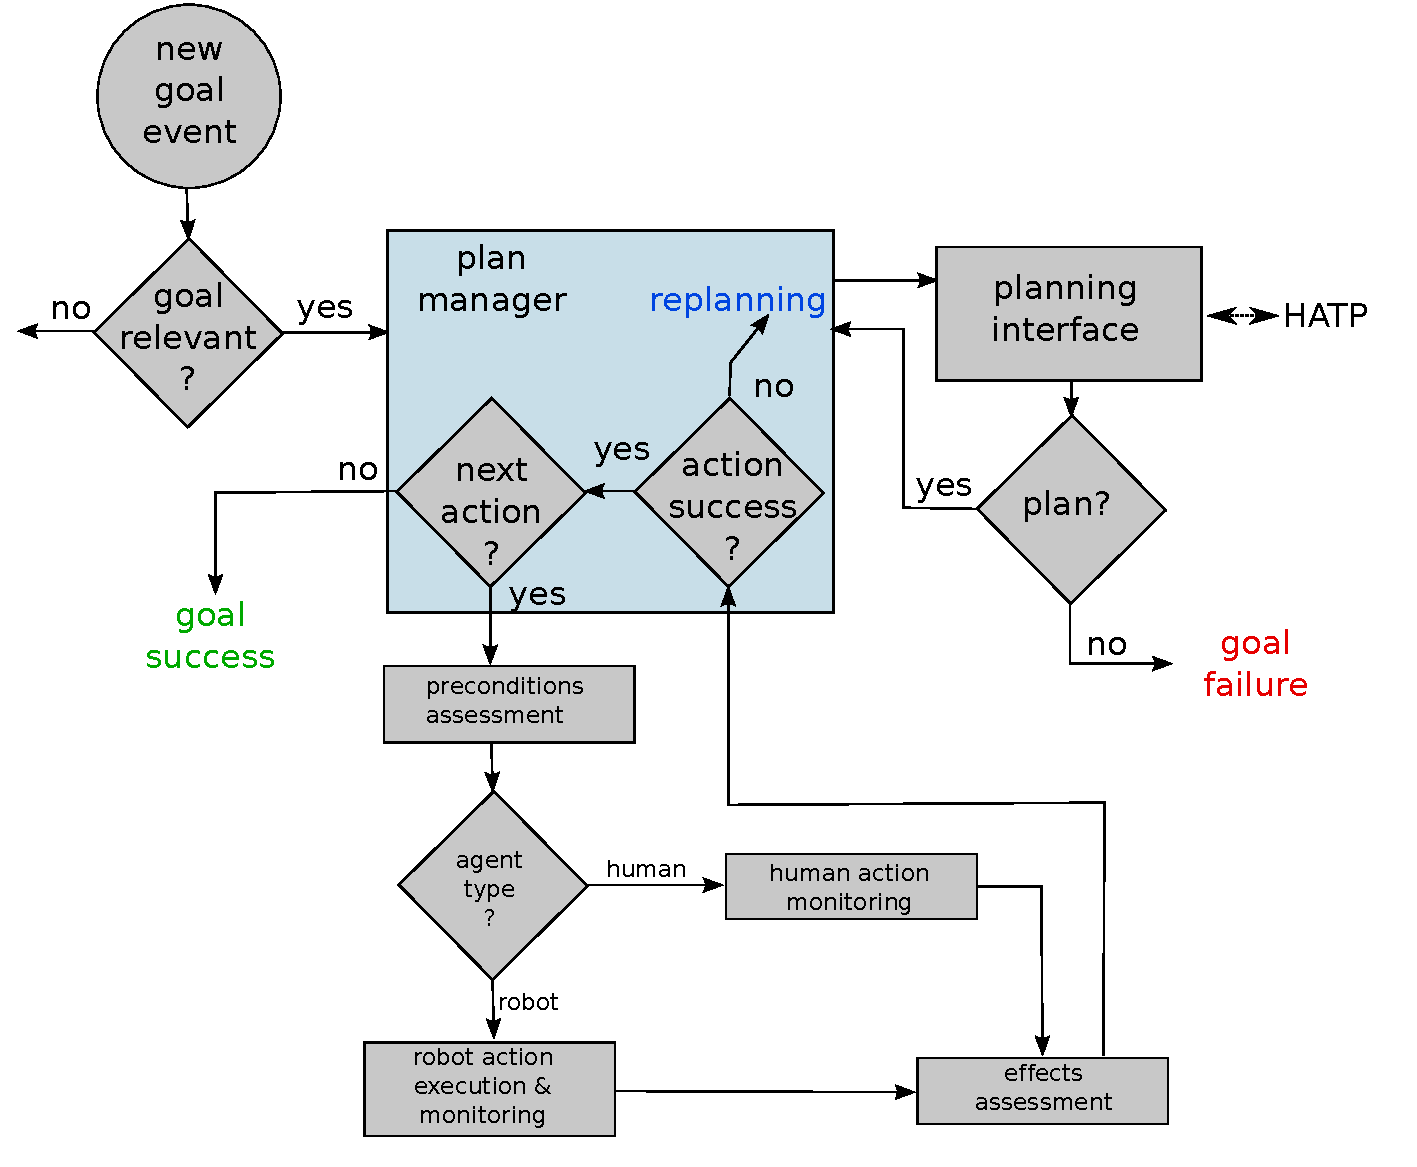
\includegraphics[width=0.8\columnwidth]{./figs/plan_management.pdf}
  \caption {Automaton for goal and plan management}
  \label{goal_plans_fg}
\end{figure}





%%%%%%%%%%%%%%%%%%%%%%%%%%%%%%%%%%%%%%%%%%%%%%%%%%%%%%%%%%%%%%%%%%%%%%%%%%%%
%%%%%%%%%%%%%%%%%%%%%%%%%%%%%%%%%%%%%%%%%%%%%%%%%%%%%%%%%%%%%%%%%%%%%%%%%%%%

\section{Second Application: Natural Language Grounding}
\label{dialog}


Verbal interaction with human presents two categories of challenges: syntactic
ones, and semantic ones. The robot must be able to process and analyze the
structure of human utterances, \ie natural language sentences, and then make
sense of them. 

In this second application of our cognitive architecture, we show how we
harness the symbolic knowledge base to ground, interpret and act on verbal
instructions.

Furthermore, this process takes full advantage of the embodied nature of the
interaction: because deitic gestures and postures are also available in the
symbolic knowledge base (as presented in section~\ref{spark-deitic}) and
dynamically updated during the interactions, verbal dialogue processing turns
into a truely multi-modal communication processing, leading to more robust
interpretation.

We present here the processing of three categories of sentences:
\emph{statements}, \emph{desires} and \emph{questions} that can be answered
from the declarative knowledge present in the robot knowledge base (a choice
similar to the \emph{Behaviour Cycle} in the GLAIR
architecture~\cite{Shapiro2009}). In our work, the grounding process of the
human discourse consists in extracting either the \emph{informational} content
of the sentence to produce statements or its \emph{intentional} content (\ie
performative value) to collect orders and questions. We do not claim any
contribution to the field of computational linguists (see \cite{Kruijff2010}
for a survey of formal approaches to natural language processing in the
robotics field). Our main contribution here is the grounding (we call it
\emph{resolution}) of concepts involved in the human discourse through the
robot's own knowledge.

\begin{figure}[!t]
\centering
  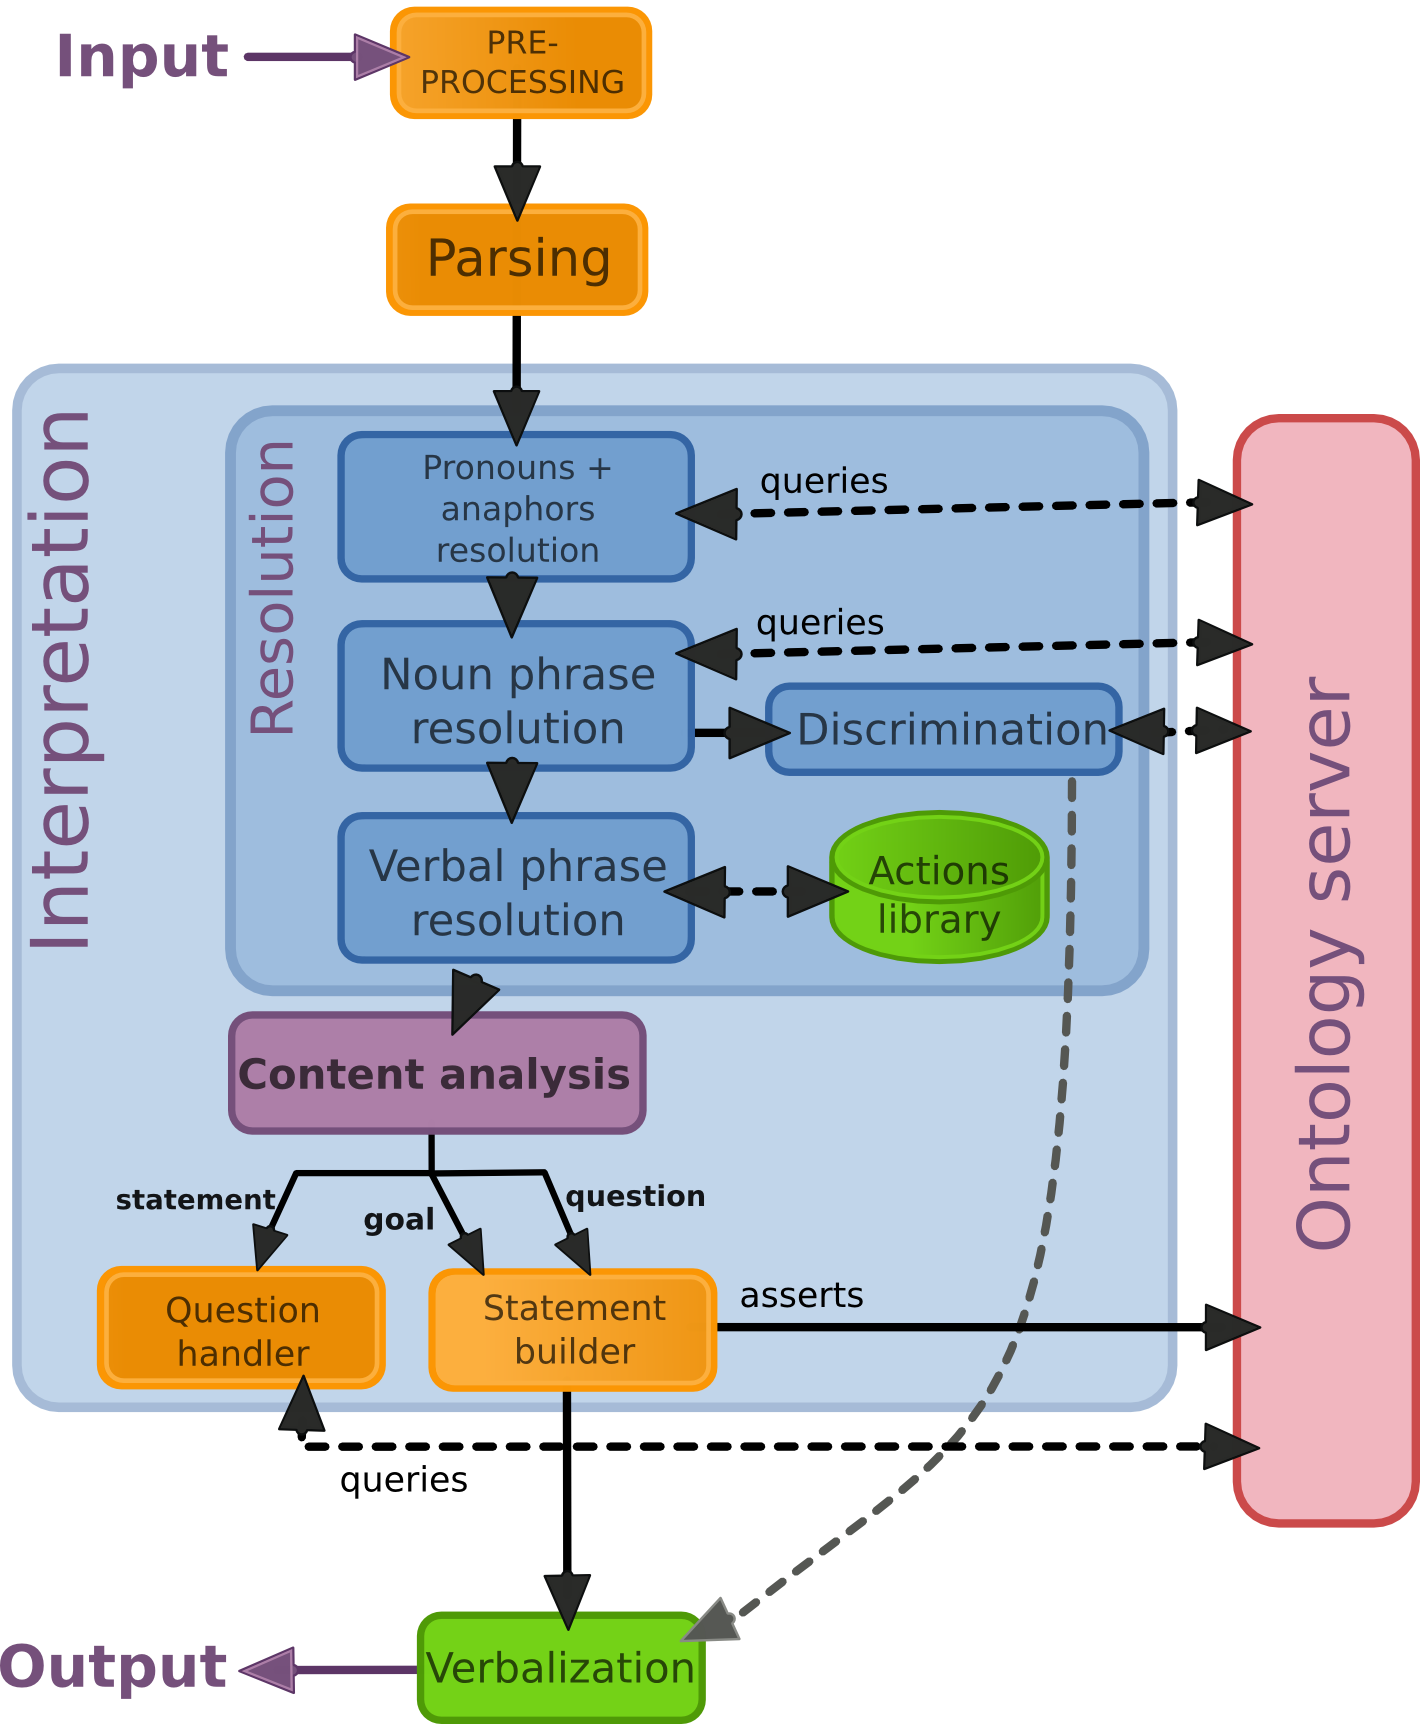
\includegraphics[width=0.9\linewidth]{figs/dialog_module_simple.png}
  \caption{The {\sc Dialogs} module has three main steps: the parsing,
  the interpretation and the verbalization. The interpretation module is
  responsible for both the \emph{resolution} and the semantic content
  \emph{analysis and translation}.} 
  \label{fig|dialog}
\end{figure}

To this end we have developed a dedicated module called {\sc Dialogs} that processes human
input in natural language, grounds the concepts in the robot's knowledge and
eventually translates the discourse in a set of queries or declarative OWL/RDF
statements. Figure~\ref{fig|dialog} shows the {\sc Dialogs} module architecture. The user's
input is first pre-processed. For instance, \emph{I'm} constructs are expanded
into \emph{I am} and then parsed. The parser is a custom-made, rule-based (\ie
grammar-free) tool that extracts the grammatical structure from the user's
sentence. Figure~\ref{dialog|parser_output} shows an example of the raw output of the parser for a moderately complex sentence.

\begin{figure}%[!ht]
\begin{center}
\scriptsize
\begin{alltt}
>> IMPERATIVE
VP: \textbf{remember} (present simple)
    SUBSENTENCE (aim: that)
      NP: \textbf{I}
      VP: \textbf{want} (present simple)
        direct objects: 
          NP: \textbf{you}
        secondary VP: \textbf{give} ()
              direct objects:
                NP: my \emph{nice blue} \textbf{bottle}
              indirect objects:
                NP: \textbf{me}
\end{alltt}
\end{center}
\caption{Raw output of the {\sc Dialogs} parser after processing the
sentence: ``remember that I want you to give me my nice blue bottle.'' 
Nominal groups are not grounded yet.} 
\label{dialog|parser_output}
\end{figure}

The output of the parser is then sent to the \emph{interpretation} module, the
core of the component.  Interpretation consists in three distinct operations:
the sentence \emph{resolution} (concepts grounding), the \emph{content
analysis} (what is the intent of the utterance: information, question or
desire) and the \emph{statement building} (translation into RDF statements).

The sentence resolution has three steps: {\it(i)} pronouns and anaphora are
replaced by the correct speaker ID and the ID of the last object referred to
(extracted from the dialogue history) respectively, {\it(ii)} nominal groups are
disambiguated and grounded (noun phrase resolution), and {\it(iii)}
verbal groups are resolved and their associated \emph{thematic roles} are
retrieved (verb phrase resolution).

\small
\begin{pseudocode}[ruled]{Resolution}{sentence, currentSpeaker}
\label{algo|Resolution}

\mathcal{G} \GETS \CALL{ParseNominalGroups}{sentence} \\

\FOREACH g \in \mathcal{G} \DO 
\BEGIN
   \mathcal{D} \GETS \CALL{GenerateDescription}{g} \STMTNUM{5.1em}{res.desc}\\
   candidates \GETS \CALL{Ontology.Find}{\mathcal{D}} \STMTNUM{4em}{res.onto}\\
   
   \IF \left|{candidates}\right| = 0 \THEN
    \BEGIN
      \OUTPUT{\mbox{Couldn't resolve the group!}} \\
      \EXIT \\
    \END
   \ELSEIF \left|{candidates}\right| = 1 \THEN
      id \GETS candidates[0]\\

   \ELSE
      \BEGIN
	\IF \CALL{Ontology.CheckEquivalent}{candidates} \THEN
	  id \GETS candidates[0] \\
	\ELSE
	  id \GETS \CALL{Discrimination}{candidates} \STMTNUM{0em}{st.discrimination}\\
      \END \\
   \CALL{Replace}{g, id, sentence}
\END
\end{pseudocode}
\normalsize

As represented in Figure~\ref{fig|dialog}, interpretation tightly relies on the
communication with the knowledge base. All the concepts the robot manipulates
are stored in the ontology server and retrieved through logical
queries, except for the verbs that are currently stored in a dedicated library
(the \emph{action library} in the diagram).

%%%%%%%%%%%%%%%%%%%%%%%%%%%%%%%%%%%%%
%\section{Technical analysis}
%\label{examples}

In order to better understand the overall process of the {\sc Dialogs} module 
and its relation with ORO, we next describe the different steps of the approach 
based on three examples. In these examples we assume that some initial facts 
are present in the knowledge base (section~\ref{modeling_real_world} discusses how 
the initial knowledge can be acquired), both in the robot's own model and in the human's model.  Since the robot tries to ground a human utterance, all queries are sent to the human model in order to interpret it from the human perspective. 

\subsection{Informational Content Extraction}
\label{informational_content_extraction}

%\begin{figure}
%    \centering
%	\begin{tabular}{p{7cm}}
%	\emph{Initial knowledge model of} \texttt{human\_01}\\
%	\hline
%    	\hspace{0.3cm}\stmt{banana\_01 type Banana} \\
%    	\hspace{0.3cm}\stmt{banana\_01 hasColor yellow}\\
%	
%	\vspace{0.5em}
%	\emph{Human input}\\
%	\hline
%	\hspace{0.3cm}``The yellow banana is big!'' \\
%
%	\vspace{0.5em}
%	\emph{Generated partial statements}\\
%	\hline
%	\hspace{0.3cm}\stmt{?obj type Banana} \\
%    	\hspace{0.3cm}\stmt{?obj hasColor yellow} \\
%    	\hspace{0.7cm}$\Rightarrow$ \concept{?obj = banana\_01}\\
%
%	\vspace{0.5em}
%	\emph{Newly created statements}\\
%	\hline
%	\hspace{0.3cm}\stmt{banana\_01 hasSize big} \\
%	\end{tabular}
%\caption{First example of natural language grounding: the nominal group ``the
%yellow banana'' is matched with the individual \concept{banana\_01}.
%``$\Rightarrow$'' represents the output of the ontology server.}
%\label{dialog|ex1}
%\end{figure}

\begin{figure}
    \centering
%	\begin{tabular}{p{0.5\columnwidth} | p{0.5\columnwidth}}}
	\begin{tabular}{l|l}
	\emph{Initial knowledge} \texttt{human\_01} &
	\emph{Human input}\\	
	
	\hline

    	\stmt{banana\_01 type Banana} &
	``The yellow banana is big!'' \\
	
    	\stmt{banana\_01 hasColor yellow} & \\
	\vspace{0.5em}\\
	\hline

	\emph{Generated partial statements} &
	\emph{Newly created statements}\\
	\hline

	\stmt{?obj type Banana} &
	\hspace{0.2cm}\stmt{banana\_01 hasSize big} \\
	
    	\stmt{?obj hasColor yellow} & \\
    	\hspace{0.2cm}$\Rightarrow$ \concept{?obj = banana\_01}\\

	\hline
	\end{tabular}
\caption{First example: content extraction.
``$\Rightarrow$'' represents the output of the ontology server.}
\label{dialog|ex1}
\end{figure}


Figure~\ref{dialog|ex1} shows a first example of human discourse grounding and
the extraction of informational content. We assume that the robot knowledge
base only contains two initial statements in the human model. The user
asserts a new one: ``The yellow banana is big!''. 
We first want to match the nominal group \emph{The yellow banana} to an already
known concept (algorithm~\ref{algo|Resolution}), and second to translate the property \emph{is big} into a predicate ({\tt hasSize}) to state its semantics. 

To resolve the nominal group \emph{The yellow banana} a set of partial
statements that describe the concept is generated based on the grammatical
parsing of the sentence (algorithm~\ref{algo|Resolution}(\ref{res.desc})). The parsed tree of each nominal group is translated into statements based on a set of rules.
In the example, a banana (\stmt{?obj type Banana})
that is yellow (\stmt{?obj hasColor yellow})\footnote{Predicates like
\concept{hasColor} or \concept{hasSize} that bind \concept{banana\_01} to
adjectives are extracted from a predefined database of $[Predicate \rightarrow
AdjectiveCategory]$, and falls back on the generic \concept{hasFeature}
predicate if the adjective is not known.}.  Based on these partial statements a
SPARQL query is sent to the ontology server to retrieve possible instances that match
the description (algorithm~\ref{algo|Resolution}(\ref{res.onto})).

In this first simple case, the concept \concept{banana\_01} is unambiguously
matched (since there is only one possible banana) and returned. Finally, we can
now add the new information provided by the human, \ie the new statement
\stmt{banana\_01 hasSize big}, to the human model in the ontology server.

% The translation of \emph{yellow} to \stmt{hasColor yellow} is not obvious: in
% the general case, we associate a adjective to the noun it characterizes with
% the \concept{hasFeature} predicate (for instance, \emph{The sight is beautiful}
% would translate to \stmt{sight hasFeature beautiful}). But we can also manually
% set the predicate associated to a category of adjectives: It is what has been
% done for the main colours. Another example is the size: for known size
% adjectives (big, small, etc.), the \concept{hasSize} predicate is being used.


\subsection{Intentional Content Through Verb Resolution}
The sentence in the first example is built with the state verb \emph{be} at
indicative. Let us examine a different example with an action verb at
imperative mode (an order): ``Give me the banana". The process is
described in Figure~\ref{dialog|ex2}.

%\begin{figure}
%    \centering
%	\begin{tabular}{p{7cm}}
%	\emph{Initial knowledge model of} \texttt{human\_01}\\
%	\hline
%    	\hspace{0.3cm}\stmt{banana\_01 type Banana} \\
%    	\hspace{0.3cm}\stmt{banana\_01 hasColor yellow}\\
%	\end{tabular} \\
%
%	\vspace{0.5em}
%
%	\begin{tabular}{p{7cm}}
%	\emph{Human input}\\
%	\hline
%    	\hspace{0.3cm}``Give me the banana.'' \\
%	\end{tabular} \\
%
%	\vspace{0.5em}
%
%	\begin{tabular}{p{7cm}}
%	\emph{Generated partial statements}\\
%	\hline
%    	\hspace{0.3cm}\stmt{?obj type Banana} \\
%	\hspace{0.7cm}$\Rightarrow$ \concept{?obj = banana\_01}\\
%
%	\end{tabular} \\
%
%	\vspace{0.5em}
%
%	\begin{tabular}{p{7cm}}
%	\emph{Newly created statements}\\
%	\hline
%    	\hspace{0.3cm}\stmt{human\_01 desires situation\_a3f74} \\
%    	\hspace{0.3cm}\stmt{situation\_a3f74 type Give} \\
%    	\hspace{0.3cm}\stmt{situation\_a3f74 performedBy myself} \\
%    	\hspace{0.3cm}\stmt{situation\_a3f74 actsOnObject banana\_01} \\
%    	\hspace{0.3cm}\stmt{situation\_a3f74 receivedBy human\_01} \\
%	\end{tabular}
%
%\caption{Second example: processing an order.}
%\label{dialog|ex2}
%\end{figure}

\begin{figure}
    \centering
	\begin{tabular}{l|l}
	\emph{Initial knowledge} \texttt{human\_01} &
	\emph{Human input}\\
	
	\hline
	
    	\stmt{banana\_01 type Banana} &
	``Give me the banana.'' \\
	
    	\stmt{banana\_01 hasColor yellow} & \\
	\vspace{0.5em}\\
	\hline
    	
	\emph{Generated partial statements} &
	\emph{Newly created statements}\\
	\hline
    	\stmt{?obj type Banana} & 
	\stmt{human\_01 desires sit\_a3} \\
	
	\hspace{0.2cm}$\Rightarrow$ \concept{?obj = banana\_01}
    	& \stmt{sit\_a3 performedBy myself} \\
    	& \stmt{sit\_a3 actsOnObject banana\_01} \\
    	& \stmt{sit\_a3 receivedBy human\_01} \\
	\end{tabular}

\caption{Second example: processing an order.}
\label{dialog|ex2}
\end{figure}


\label{processing_of_actions}

In order to capture the intentional content of a sentence (for example, an
order) we need to retain the semantics of the verb and its complements.
\emph{Thematic roles} allow for semantically linking a verb to its complements.  
There is no general agreement amongst linguists on a comprehensive list of 
thematic roles. The amount and the granularity of roles varies a lot in 
the literature~\cite{Gutierrez2001}. We thus use a small set of them, which matches
the relations the robot can actually achieve (we discuss
possible extensions in the conclusion). For instance, in the second example,
the verb \emph{give} has three thematic roles: \concept{performedBy},
\concept{actsOnObject} and \concept{receivedBy}.

The list of actions the robot can plan for (currently \emph{take},
\emph{place}, \emph{give}, \emph{show}, \emph{hide} and \emph{move}) along with
possible synonyms (for example, \emph{to pick} is set as a synonym of \emph{to
take}) and their associated thematic roles are stored in a predefined library
of actions. For each action we identify and store: the role of the subject in
the sentence (always \concept{performedBy}); the role of the direct object
(for instance, \concept{actsOnObject}); and the role of each of the indirect
objects with their optional prepositions (for instance,
\concept{receivedBy})\footnote{Note that in example 2, ``give me the banana'',
the pronoun ``me'' appears before ``banana'', while it is an indirect
complement --- ``give it {\bf to me}''. The parser correctly handles these
cases.}. Moreover, through the ontology we check that each holder of a
role is semantically consistent. For instance, the action \emph{Give} must have a
manipulable physical item (\concept{Artifact}) as direct object. Thus, if the
concept the robot finds for the thematic role \concept{actsOnObject} cannot be
inferred to be an artifact, the robot goes back to the human saying it does not
understand.

This second example  also shows the pronoun reference resolution: ``me'' is
replaced by the id of the current speaker, while ``you'' is replaced by
\concept{myself} (\concept{myself} always represents the robot itself). When
present, anaphoras (references to previous concepts like ``give me the banana, I
like {\bf it}.'') are also resolved in the same step.

Once the sentence is completely resolved and translated into a formal
representation (a human desire in this example\footnote{Orders are here
represented as human desires: the human desires a specific new situation.}), we
store it in the ontology server. The robot's decisional/executive layers can
then decide whether to execute the order or not. 

\subsection{Informational Content Extraction Requiring Clarification}
\label{dialogs:disamb}
\begin{figure}
    \centering
	\begin{tabular}{p{7cm}}
	\emph{Initial knowledge model of} \texttt{human\_01}\\
	\hline
     	\hspace{0.3cm}\stmt{banana\_01 type Banana} \\
     	\hspace{0.3cm}\stmt{banana\_01 hasColor yellow} \\
     	\hspace{0.3cm}\stmt{banana\_02 type Banana} \\
     	\hspace{0.3cm}\stmt{banana\_02 hasColor green} \\
	\end{tabular} \\

	\vspace{0.5em}

	\begin{tabular}{p{7cm}}
	\emph{Human input}\\
	\hline
     	\hspace{0.3cm}``The banana is good.'' \\
	\end{tabular} \\

	\vspace{0.5em}

	\begin{tabular}{p{7cm}}
	\emph{Generated partial statements}\\
	\hline
     	\hspace{0.3cm}\stmt{?obj type Banana} \\
	\hspace{0.7cm} $\Rightarrow$ \concept{?obj = [banana\_01, banana\_02]}
	\end{tabular} \\

	\vspace{0.5em}

	\begin{tabular}{p{7cm}}
	\emph{Discrimination process}\\
	\hline
     	\hspace{0.3cm}\concept{discriminate([banana\_01, banana\_02])} \\
	\hspace{0.7cm} $\Rightarrow$ \concept{?hasColor = [yellow, green]}
	\end{tabular} \\

	\vspace{0.5em}

	\begin{tabular}{p{7cm}}
	\emph{Robot output speech}\\
	\hline
     	\hspace{0.3cm}``The yellow one or the green one?'' \\
	\end{tabular} \\

	\vspace{0.5em}

	\begin{tabular}{p{7cm}}
	\emph{Human answer}\\
	\hline
     	\hspace{0.3cm}``The green one.'' \\
	\end{tabular} \\
    
	\vspace{0.5em}

	\begin{tabular}{p{7cm}}
	\emph{Extended human input}\\
	\hline
     	\hspace{0.3cm}``The green banana is good.'' \\
	\end{tabular} \\
	
	\vspace{0.5em}

	\begin{tabular}{p{7cm}}
	\emph{Generated partial statements}\\
	\hline
     	\hspace{0.3cm}\stmt{?obj type Banana} \\
     	\hspace{0.3cm}\stmt{?obj hasColor green} \\
	\hspace{0.7cm} $\Rightarrow$ \concept{?obj = [banana\_02]}
	\end{tabular} \\
    
	\vspace{0.5em}
	\begin{tabular}{p{7cm}}
	\emph{Newly created statements}\\
	\hline
     	\hspace{0.3cm}\stmt{banana\_02 hasFeature good} \\
	\end{tabular}

\caption{Ambiguity resolution: in this example, ``banana'' can refer to the
yellow banana (\concept{banana\_01}) or the green one (\concept{banana\_02}).
Discrimination routines handle the disambiguation process.} \label{dialog|ex3}
\end{figure}

This last example (Figure~\ref{dialog|ex3}) shows the resolution of ambiguous
concepts. In this case the user refers to ``the banana'' while two instances of 
the \concept{Banana} class exist in the ontology. The robot needs to find out
to which instance the user is actually referring to. To this end,
disambiguation routines (algorithm~\ref{algo|Resolution}(\ref{st.discrimination}), see \cite{Ros2010b} for details of the routines)
find differences between the instances (in the example, one banana is yellow
while the other one is green) and build a sentence through the
\emph{verbalization} module to ask the user a closed question that will
help clarify the ambiguity: ``Is it yellow or green?'' The user's answer is
parsed and merged with the previous sentence. The resulting, augmented,
sentence (``The green banana is good") goes again through all the
interpretation steps. This process is repeated until no ambiguities arise. 
In the example, the \concept{banana\_02} is finally returned.

%If no differences \fxfatal{should we say 'in the human model', even if 
%getDiscriminantForAgent currently doesn't work?} can be found, an open question 
%(``give me more information'') is send to the human.

Several other strategies are used in parallel to disambiguate concepts without
having to ask for more information to the human:

\begin{itemize}
	\item Which objects are currently visible to the human? If only one of
	them, then it is probably the one the user is talking about. 
	\item Did a previous interaction involved a specific object that would
	still be the subject of the current sentence?
	\item Is the user looking or pointing at a specific object?
\end{itemize}

%Two cases can alter the way the discrimination routines work:
%\begin{enumerate}
%    \item If a sentence starts with {\it Learn that...}, failures during 
%    discrimination are interpreted as new concepts, and instead of marking the 
%    nominal as not resolved, and new identifier is created and add to the knowledge base.
%    \item For questions like {\it Which color is the bottle?}, the discrimination 
%    algorithm can not use the feature {\it color} to identify to bottle. The 
%    resolution algorithm pass this kind of constraints as a parameter of the 
%    discrimination routines.
%\end{enumerate}

 
While no examples involving questions have been detailed, factual \emph{wh-}
questions and polar (\emph{yes/no}) questions can be processed in a similar way
by \textsc{Dialogs}. For instance, a question like ``What is on the table?'' is
grounded (to extract the relation \concept{isOn} and to find what \emph{table}
refers to) and transformed into the following kind of query: \concept{find ?var
[\stmt{?var isOn table1}]}.  Answers are converted back to a full sentence by
the \emph{verbalization} module, and uttered to the human.






%%%%%%%%%%%%%%%%%%%%%%%%%%%%%%%%%%%%%%%%%%%%%%%%%%%%%%%%%%%%%%%%%%%%%%%%%% 
%%%%%%%%%%%%%%%%%%%%%%%%%%%%%%%%%%%%%%%%%%%%%%%%%%%%%%%%%%%%%%%%%%%%%%%%%% 

%\section{Experiments}
%\label{experiments}

%This section presents several experiments where the different features of our
%approach are represented. The experiments have been conducted on two different
%platforms: the \emph{Rosie} manipulator from the Technical Universtiy of
%Munich, a dual-arm, holonomic service robot, running the
%ROS\footnote{\emph{Robotic Operating System}, \url{http://www.ros.org}}
%middleware; and the \emph{Jido} robot~\cite{Alami1998a} from LAAS-CNRS, a
%similar, single-arm, service robot, running the LAAS's {\sc Genom/pocolibs}
%stack. Both platforms share the use of ORO, the ontology server described in
%this work.

%\subsection{\emph{Naming} Experiment}
%\label{naming}

%\begin{figure}
%\centering
%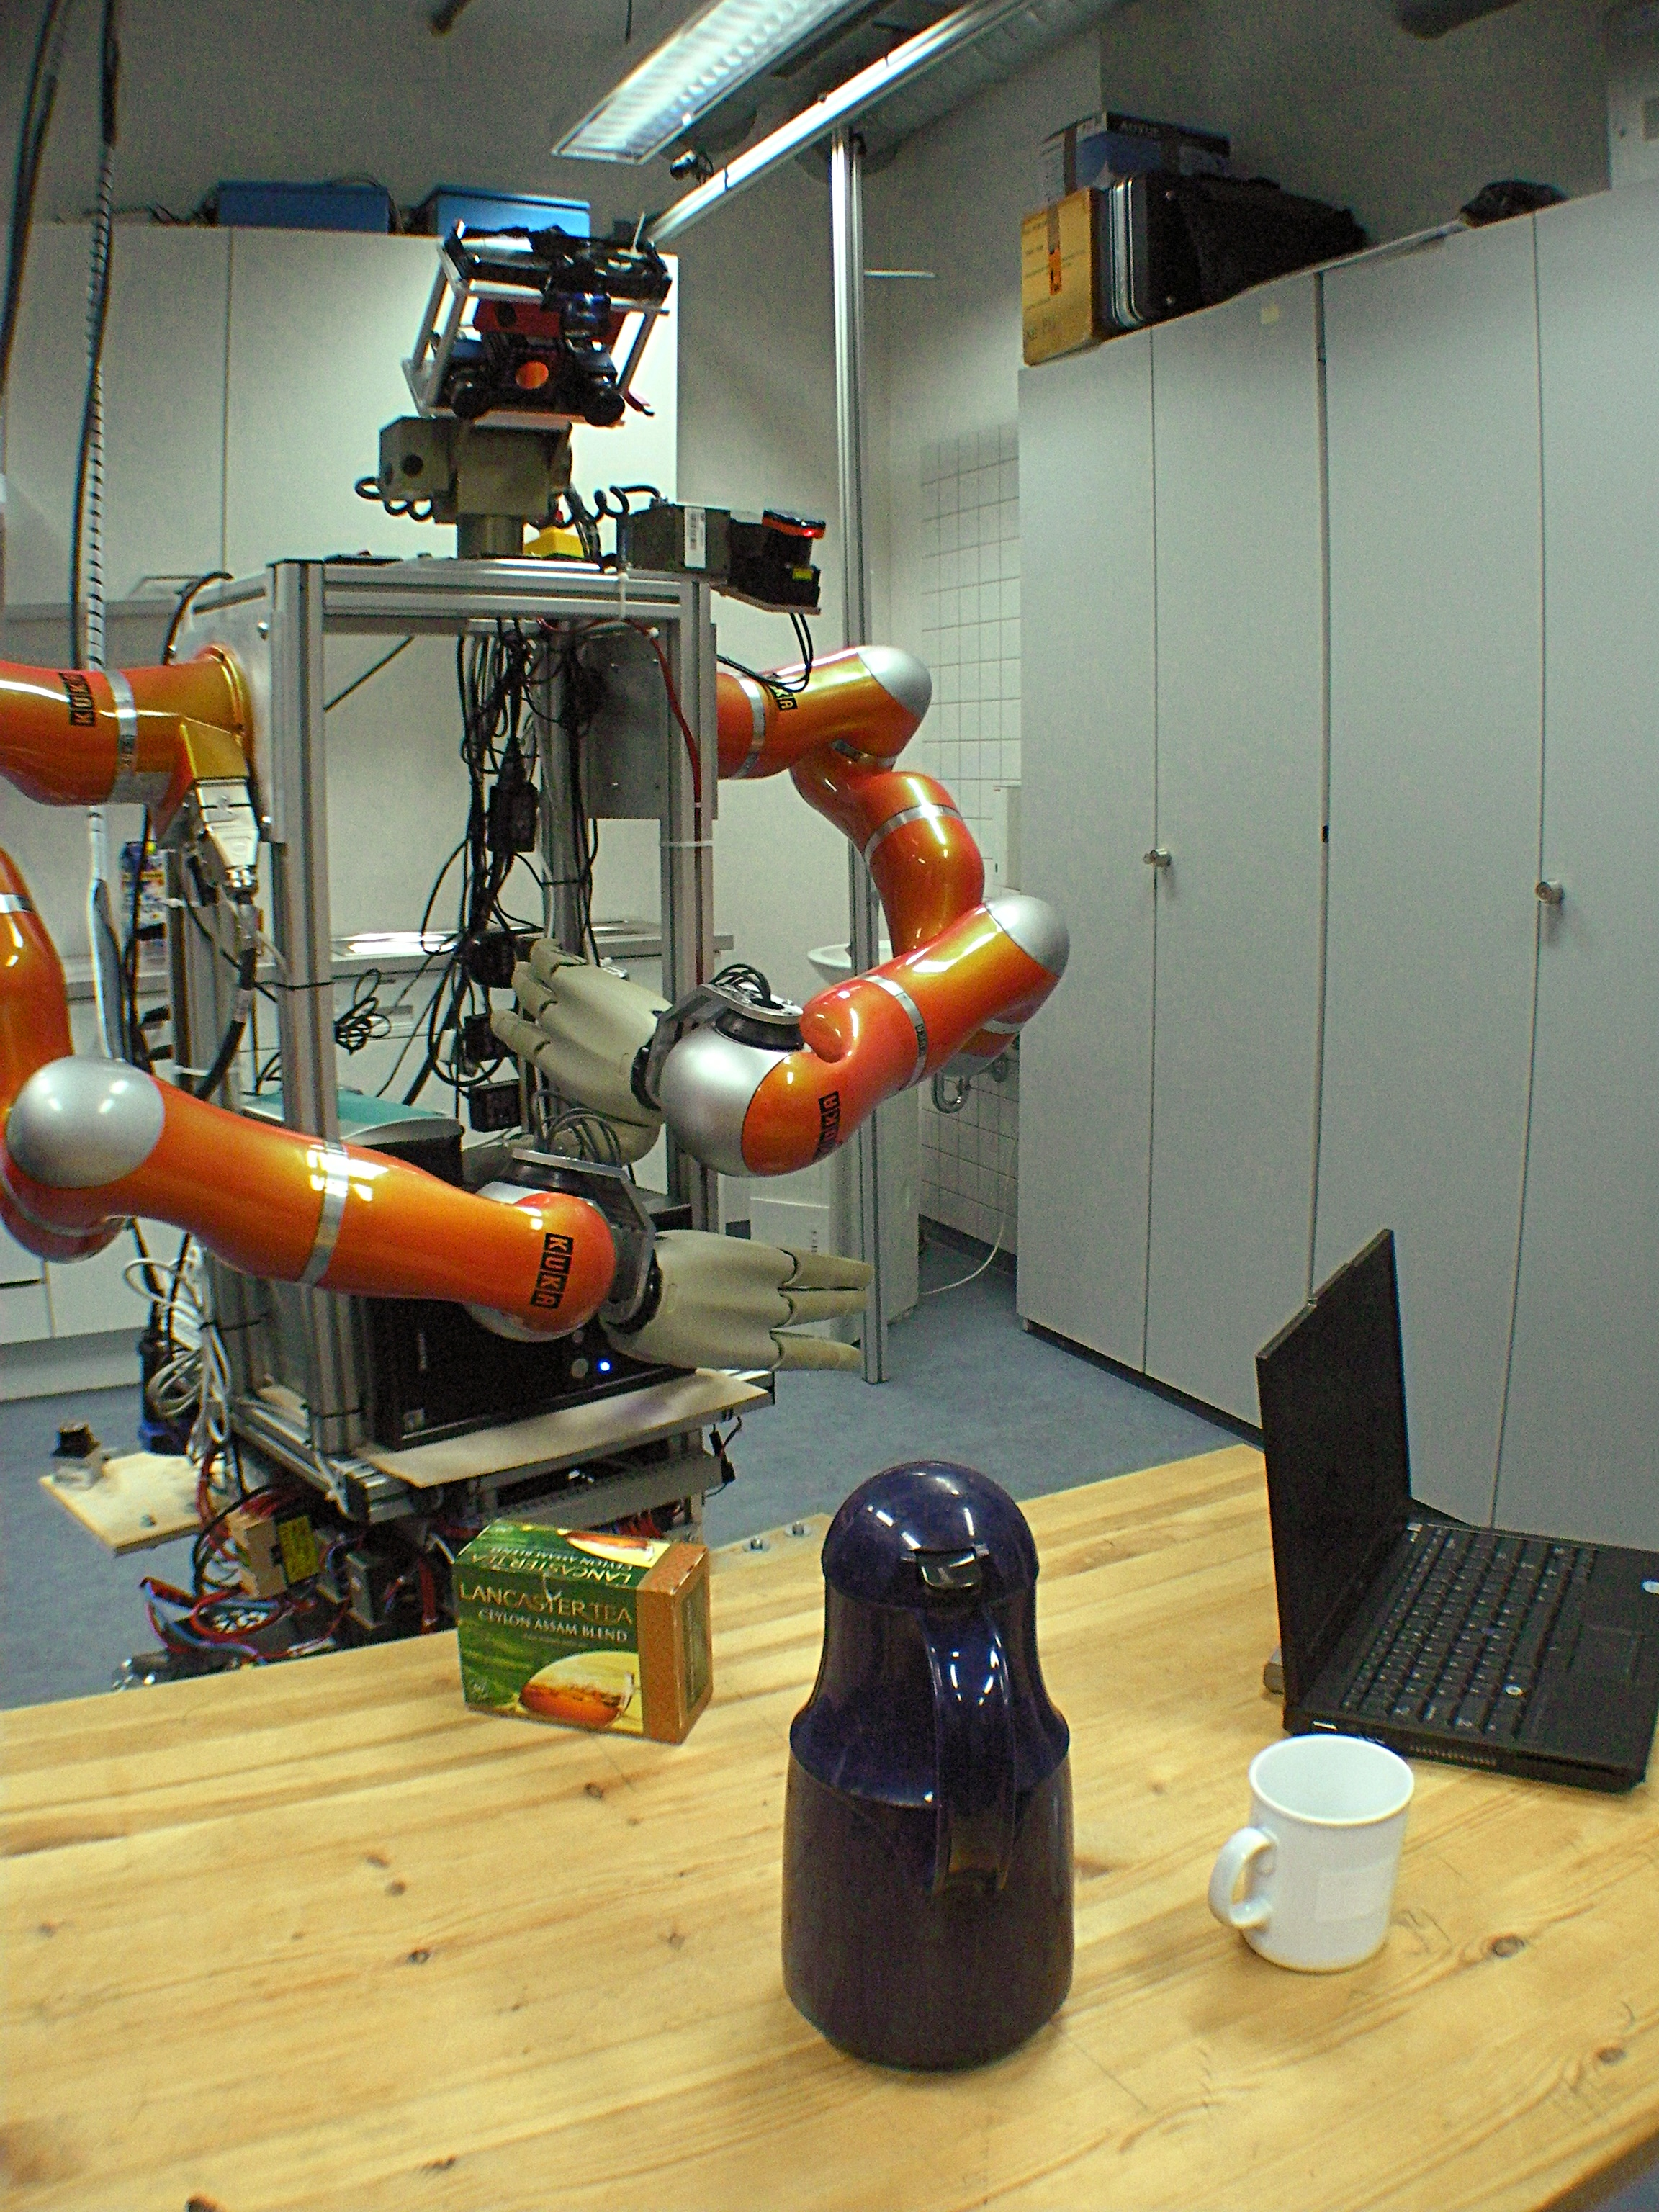
\includegraphics[width=0.45\columnwidth]{figs/kimp1.jpg}
%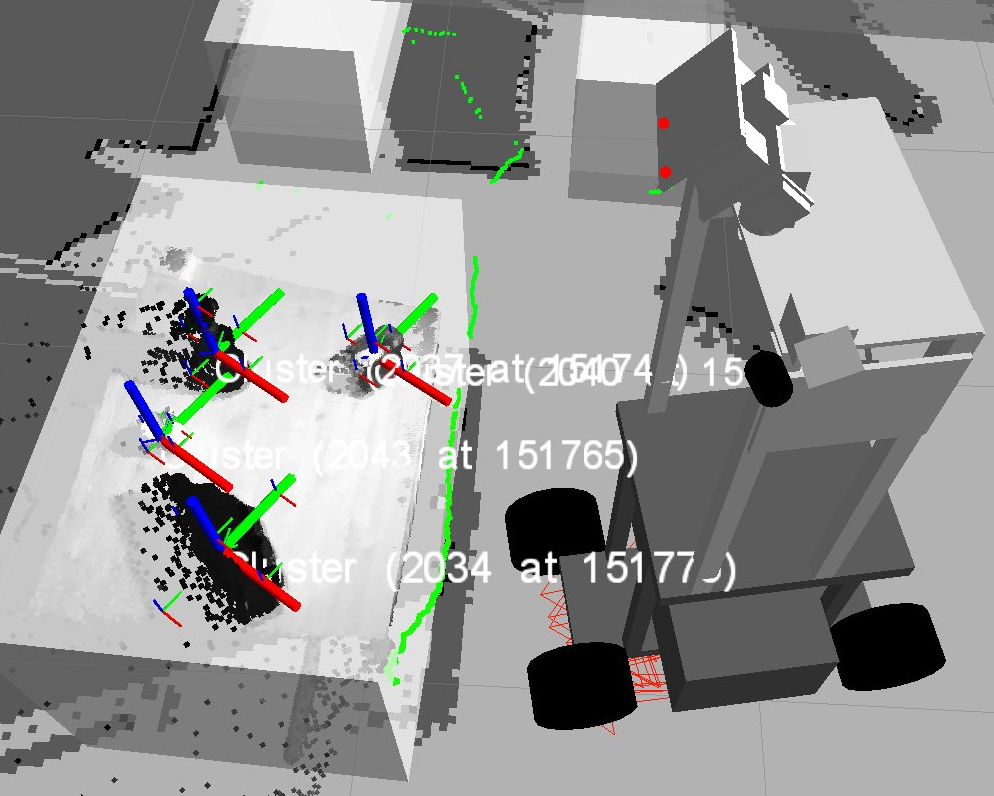
\includegraphics[width=0.45\columnwidth]{figs/rviz.png}
%%\parbox[c]{4.3cm}{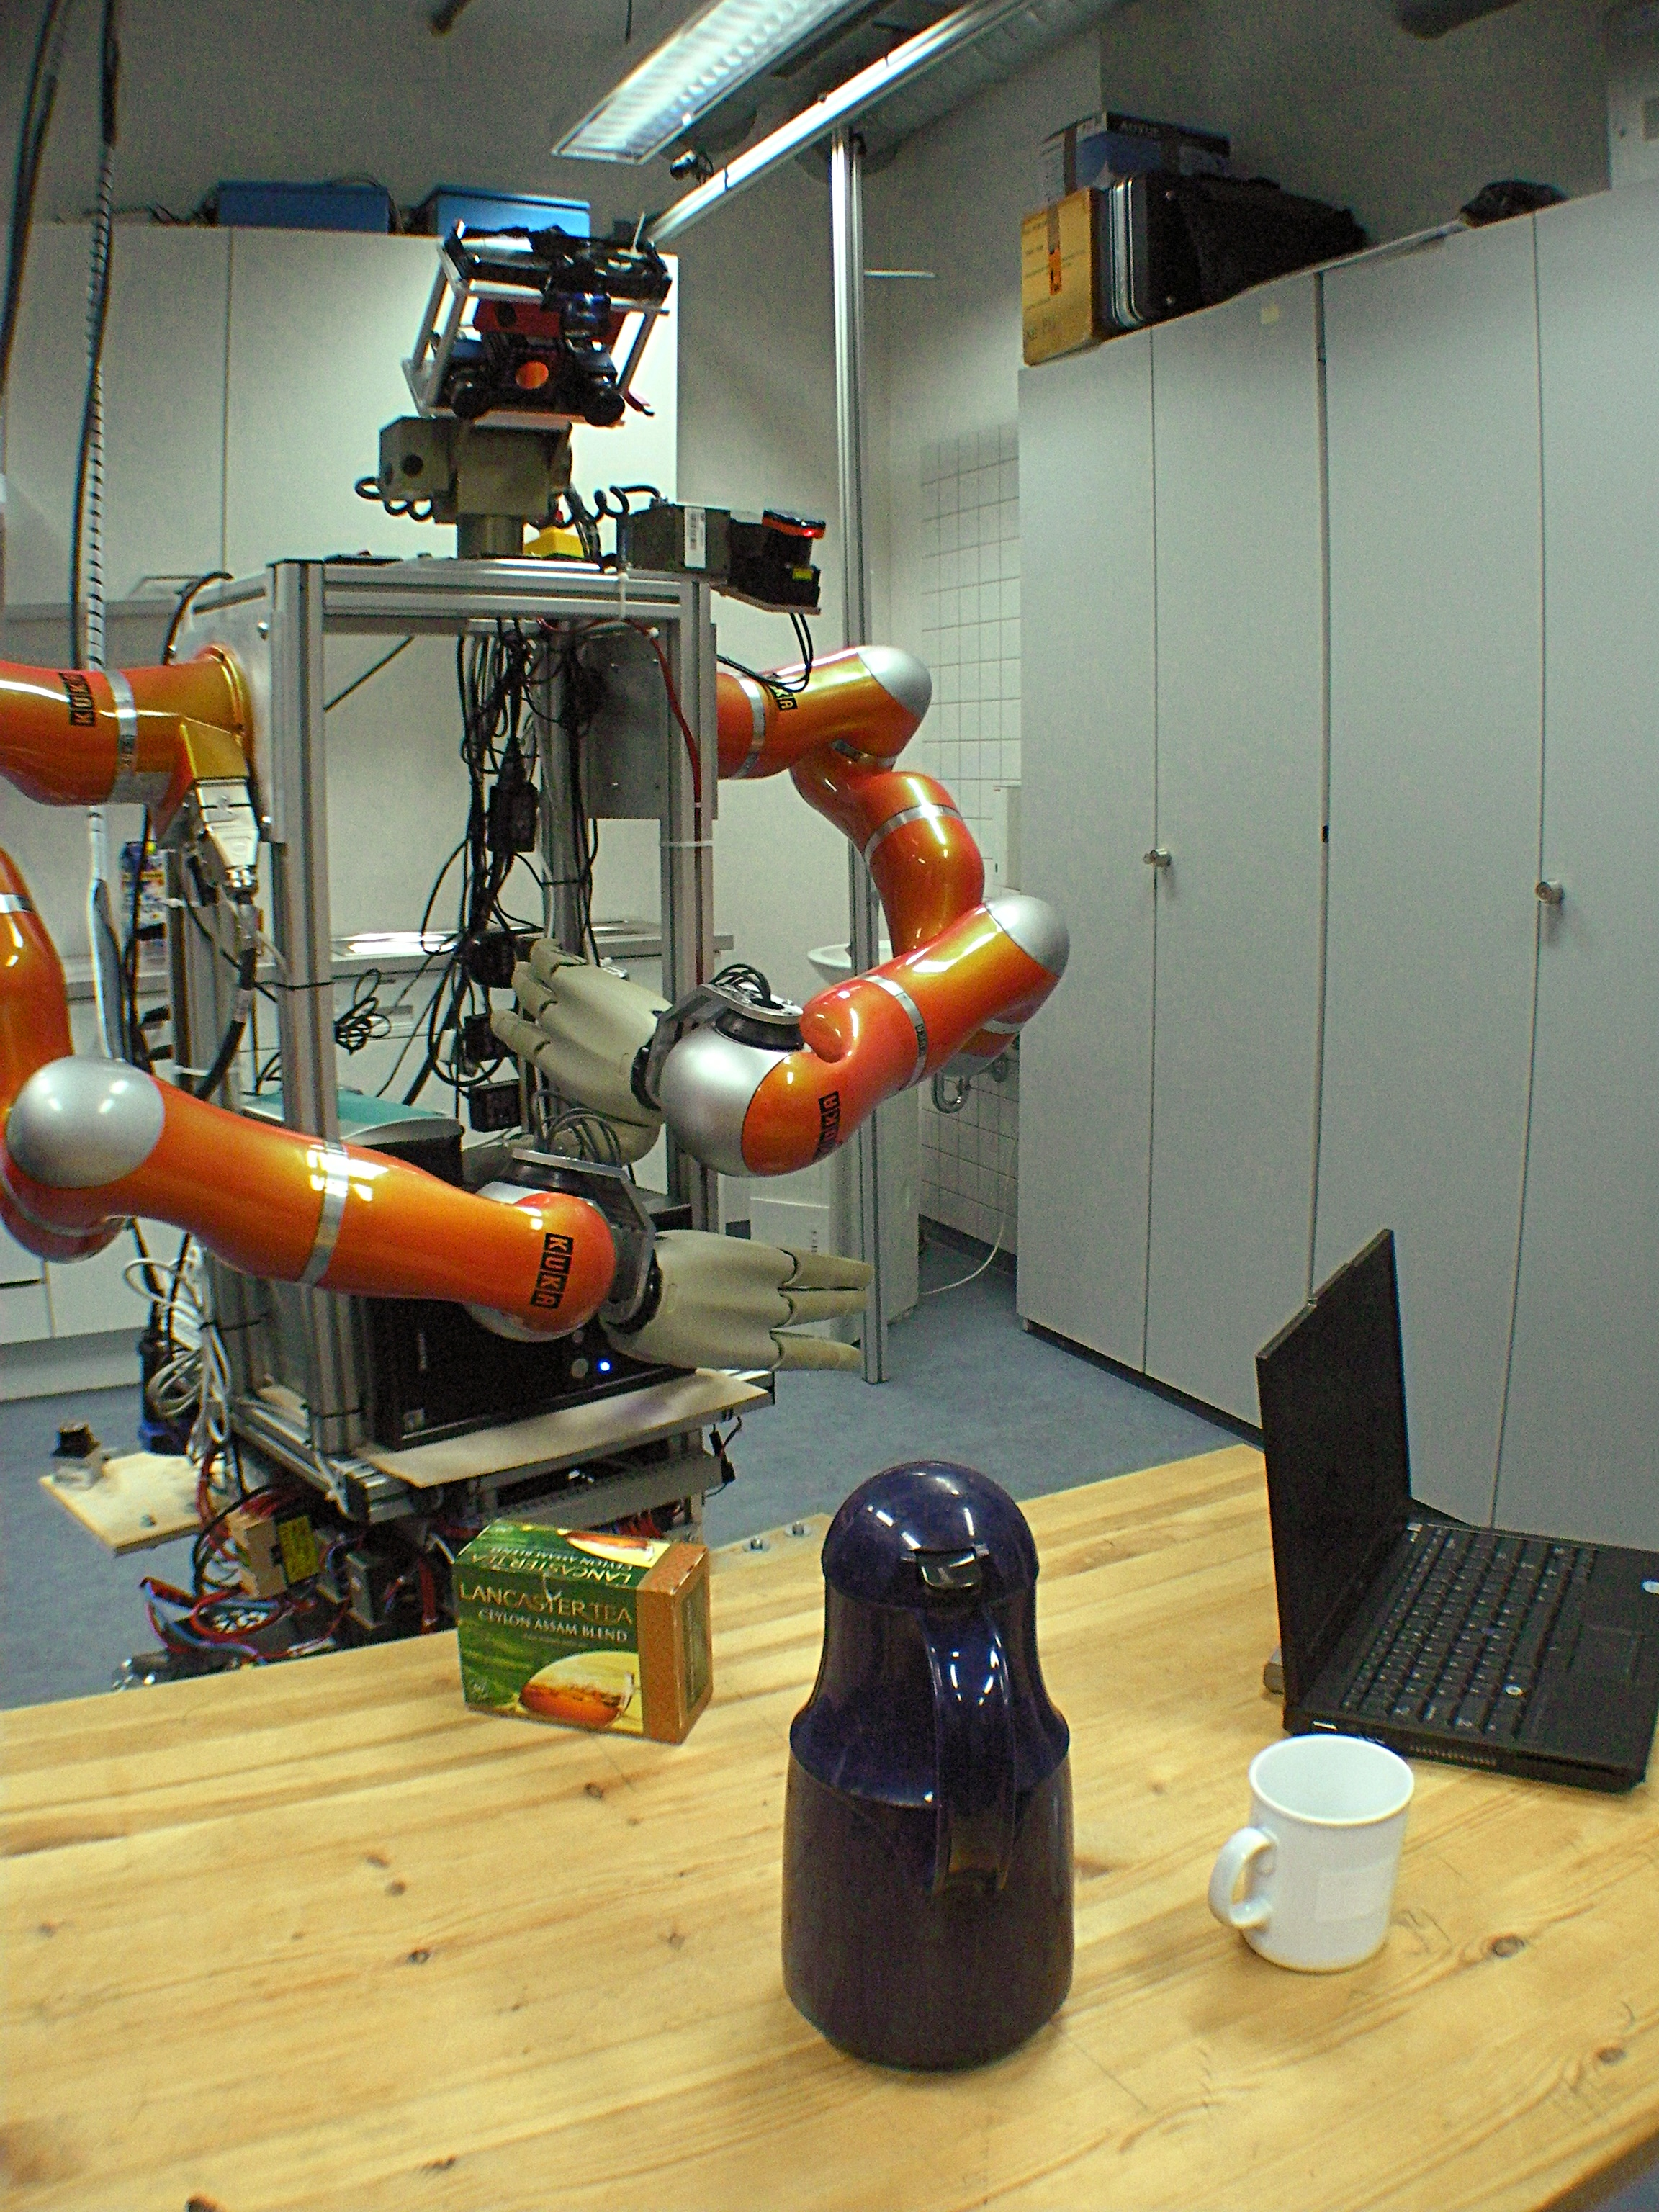
\includegraphics[width=0.5\columnwidth]{figs/kimp1.jpg}}
%%\parbox[c]{4.1cm}{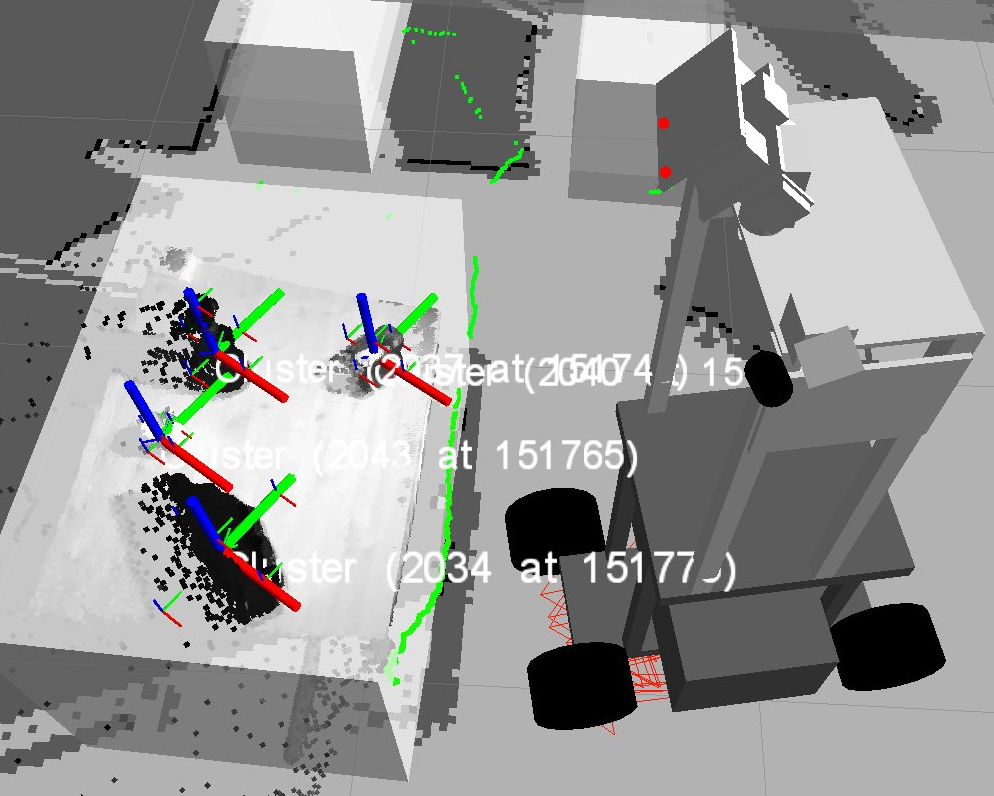
\includegraphics[width=4cm]{figs/rviz.png}}
%\flushleft
%\hspace{1.8cm} (a) \hspace{3.9cm} (b)
%\caption{(a) Rosie, looking for objects it may know, and (b) view from Willow
%Garage's RViz. The clusters of point are given a unique identifier by the
%perception module. This allows the supervision module to create the link between the physical
%objects and their symbolic representation in ORO.} 
%\label{fig|kimpwatching}
%\end{figure}

%The \emph{Naming} task uses ORO to anchor perception into the robot's knowledge
%through interaction with the user. This task has been implemented on the Rosie
%robot at TU Munich.

%The robot selects an unknown object from the table, shows it to the user, and
%asks about its name and type (Figure~\ref{fig|kimpwatching}). The user
%interacts with the robot through a dedicated bridge, allowing him/her to chat with
%the robot with a standard Jabber instant messaging client.
%Figure~\ref{tab|transcript_kimp} shows a chat session with Rosie performing the
%naming experiment. The human describes the object until the robot recognizes a
%type it already knows. More precisely, the robot recursively asks the human for the categories the object belongs to until reaching a known one. At this point, the robot is able to connect the new object information to already known concepts. Therefore, the robot
%accurately anchors perception in its symbolic model and it is able to reason
%about it.  The learning process starts over again with each unknown object. To
%further exploit the knowledge reasoner in this experiment, we ask the robot
%which object does not belong to a typical breakfast table, \ie we ask for the odd
%objects. In this case, it corresponds to objects that are neither of type
%\concept{Tableware} nor \concept{Food}. 

%The supervision module (\textsc{cram}\footnote{\textsc{cram} (Cognitive Robotic
%Abstract Machine) is a RPL-derived framework for rapid development of cognitive
%robot control programs we currently develop.}~\cite{Beetz2010}) automatically
%updates the ORO server whenever an object enters or leaves the field of view.
%%(the perception is based on the \textsc{CoP} framework~\cite{Klank2009}). 
%Therefore, the integration of ORO can be seen as an extension of
%the robot's belief state that not only contains abstract identifiers
%of the internal object representation used in plans, but also the
%semantics and roles of objects in the scenario.

%\begin{figure}%[!ht]
%\centering
	%\begin{tabular}{r|p{7cm}}
	%\chatN{rosie} & Servus! The Bavarian robot is up and fit! \\
	%\chatN{rosie} & What is the name of the white cluster on the table? \\
	%\chatN{human} & ``Rosie's mug'' \\
	%\chatN{rosie} &\emph{[\stmt{obj\_01 label "Rosie's mug"} added]}\\
				%& What kind of object is ``Rosie's mug''? \\
	%\chatN{human} & Mug \\
	%\chatN{rosie} & \emph{[\stmt{obj\_01 type Mug} added]}\\
			%& What is a Mug?\\ 
	%\chatN{human} & Tableware\\
	%\chatN{rosie} & \emph{[\stmt{Mug subClassOf Tableware} added. Rosie already
	%knows about \emph{Tableware} (it belongs to the common-sense ontology), so
	%the description of this object ends.]}\\
	%& (...) \\
	%\chatN{rosie} &  What is the name of the black cluster on the table? \\
	%\chatN{human} & ``my\_laptop'' \\
	%\chatN{rosie} & What kind of object is ``my\_laptop''? \\
	%\chatN{human} & Computer \\
	%\chatN{rosie} & What is a Computer? \\
	%\chatN{human} & Artifact \\
	%\chatN{rosie} & Do you want me to learn more objects? \\
	%\chatN{human} & no \\
	%\chatN{rosie} & These objects are odd: ``my\_laptop'' \\
	%\end{tabular}
	%\caption{Transcript of a Jabber session with the robot Rosie.}
	%\label{tab|transcript_kimp}
%\end{figure}

%% An unexpected example of what the symbolic reasoning layer brings to more
%% traditional robotic architectures emerged during the \emph{Naming} experiment:
%% the perception routines provided segmented blobs corresponding to objects along
%% with their colors to update the information in ORO. At some point, ORO suddenly
%% refused to add an object. What seemed at first a communication bug between
%% modules, was actually the consequence of a consistency check by ORO: because of
%% bad light conditions, the color recognition was not very reliable, and the same
%% object was set to have two different colors at the same time. Since the
%% \concept{hasColor} predicate we had decided to use was a functional predicate
%% (\ie objects can have only one color), ORO inferred an inconsistency and
%% discarded the new fact. This kind of logical failure can be used to improve
%% low-level perception outcomes by ``closing the loop'' with high-level, symbolic
%% knowledge.

%\subsection{\emph{Spy Game} Experiment}
%\label{spygame}

%This game is based on the traditional children game ``I Spy''. The idea is to
%discover the object or concept one of the participants is thinking of by asking
%questions such as: ``Is it green? Is it a machine? Is it on your left?'', etc.
%When playing, children exploit their knowledge about the world while
%categorizing and describing objects through useful discriminants that will
%allow them to find out the answer as fast as possible while including
%perspective taking abilities~\cite{Moll2006}.

%\begin{figure}
%\centering
%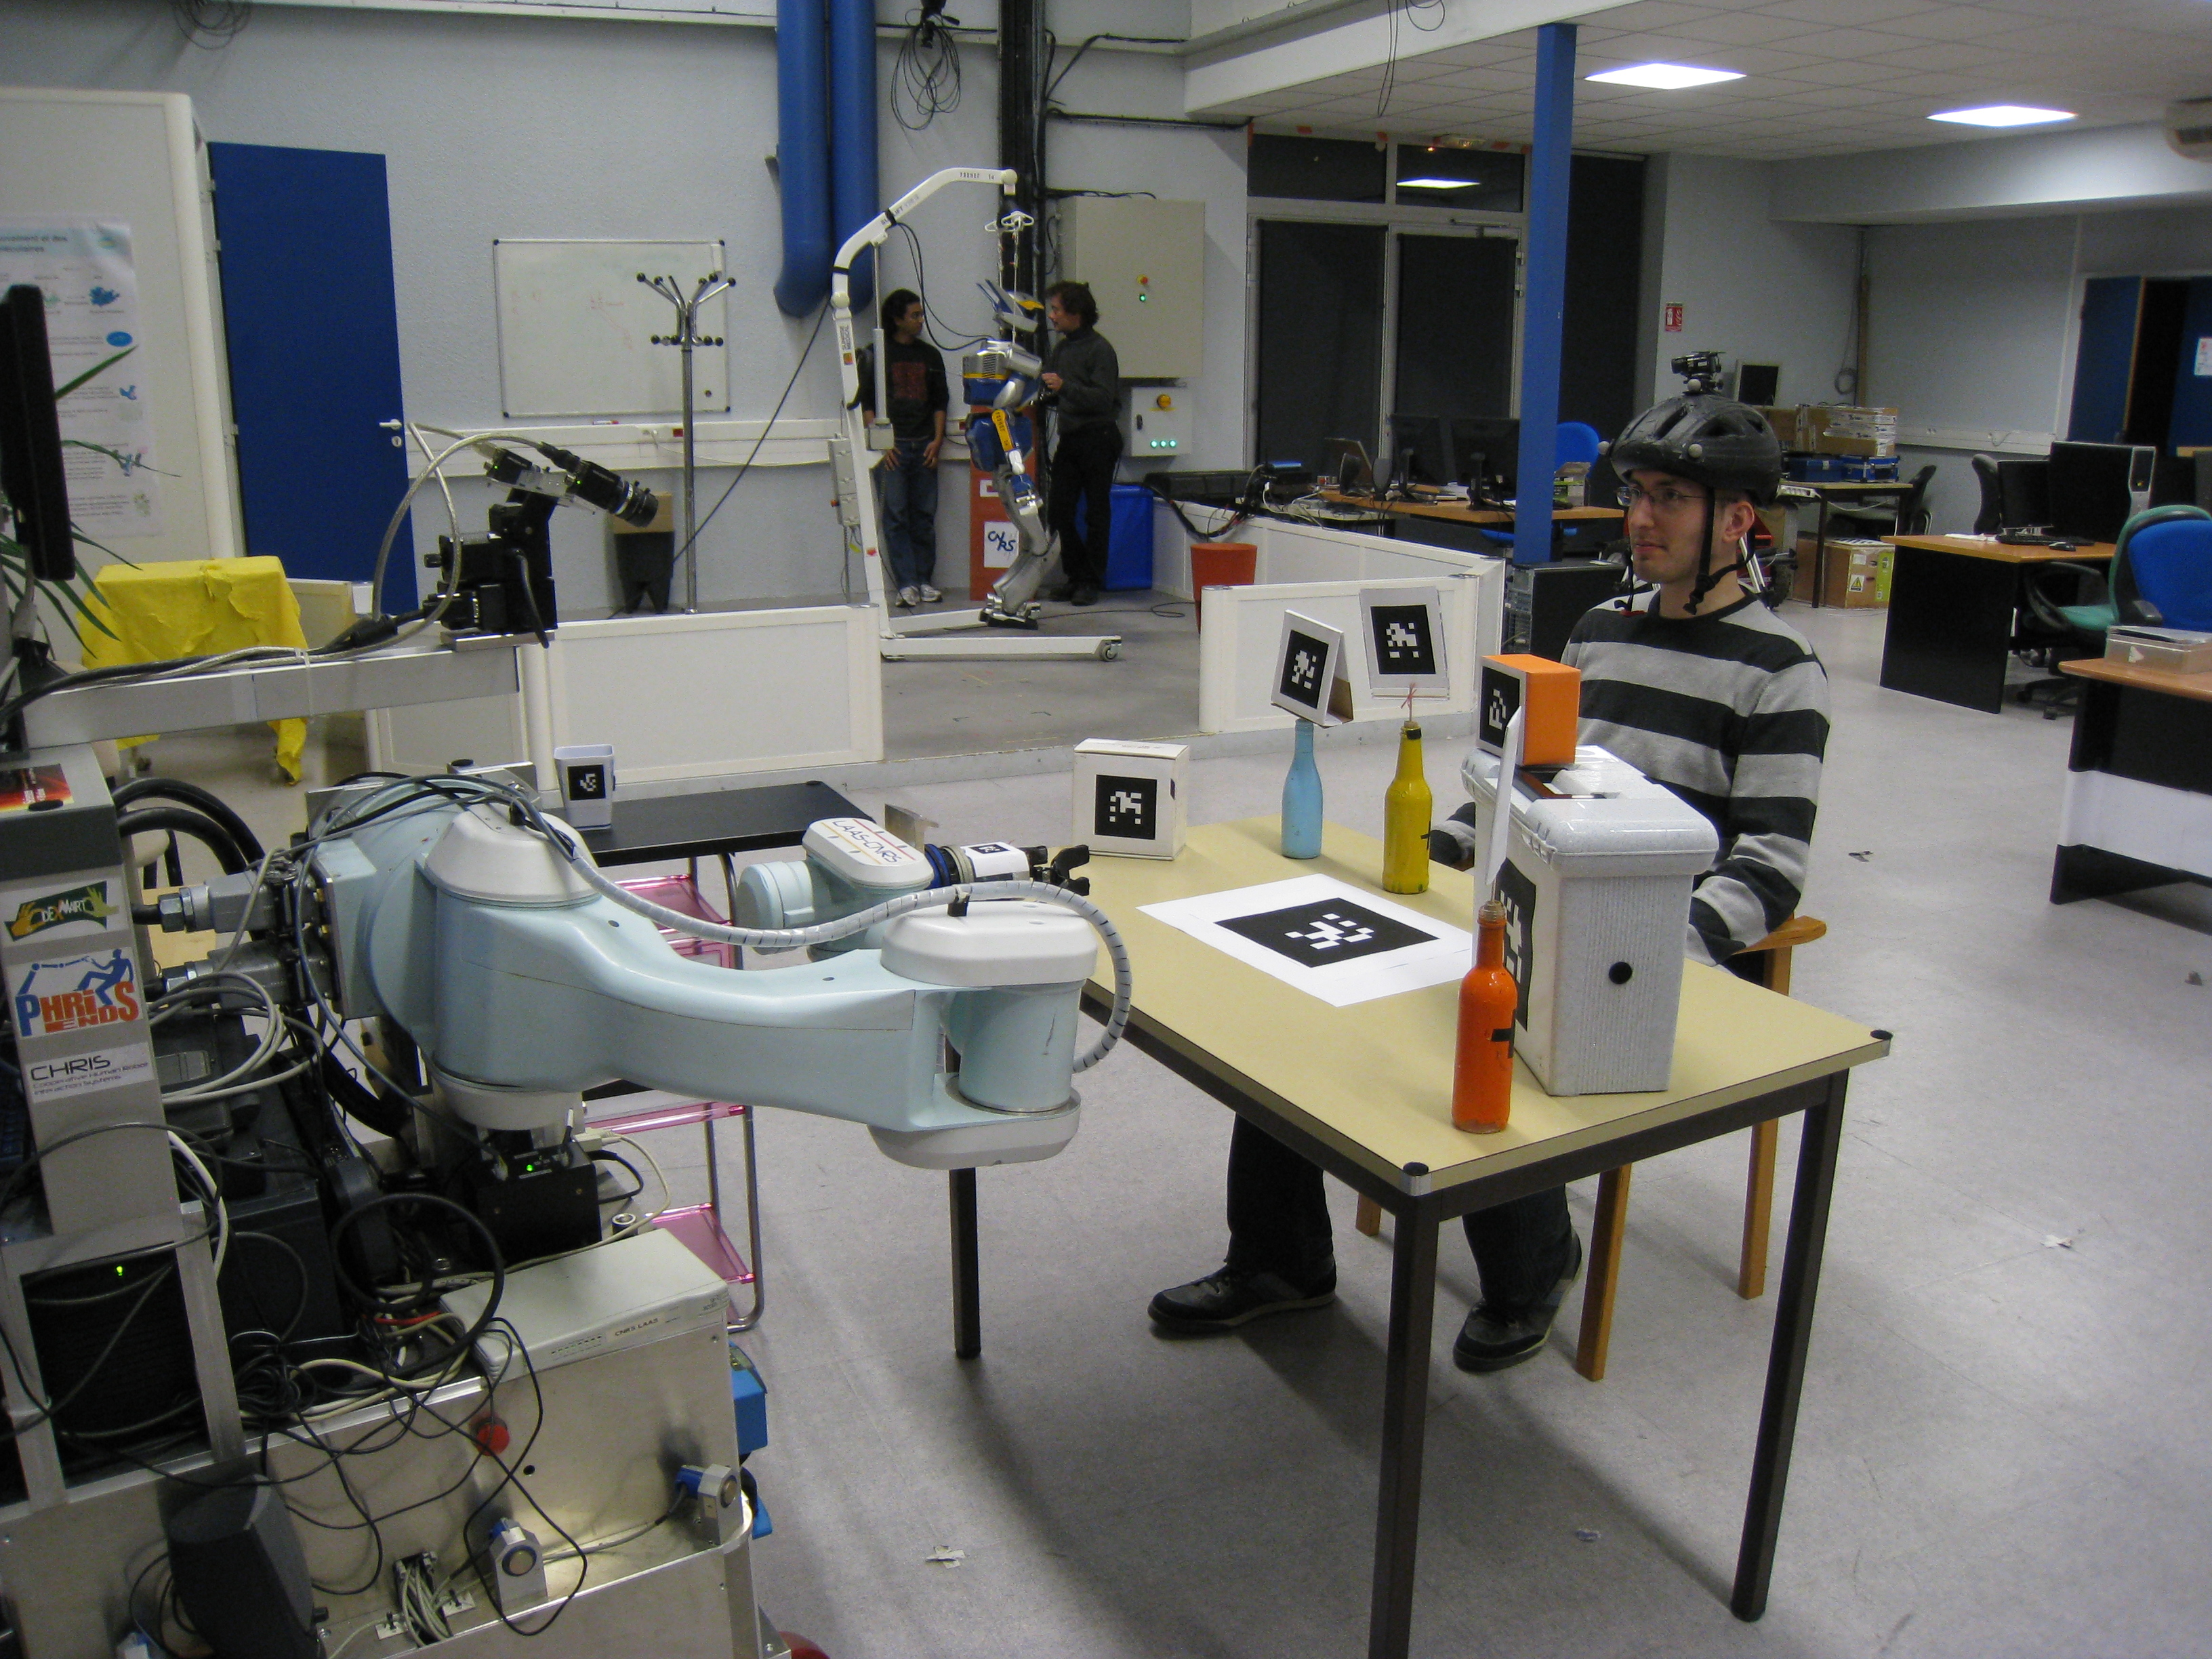
\includegraphics[width=0.45\columnwidth]{figs/spy-game-real.jpg}
%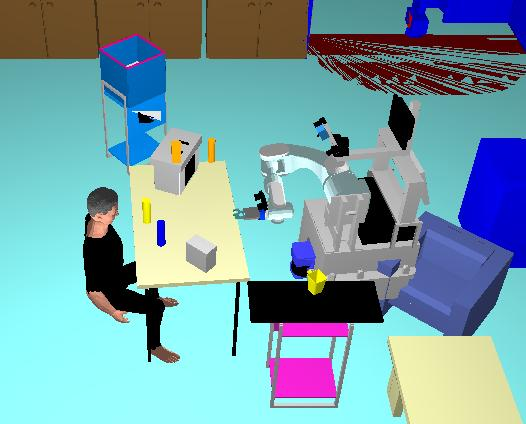
\includegraphics[width=0.45\columnwidth]{figs/spy-game-mhp.jpg}
%%\parbox[c]{4.3cm}{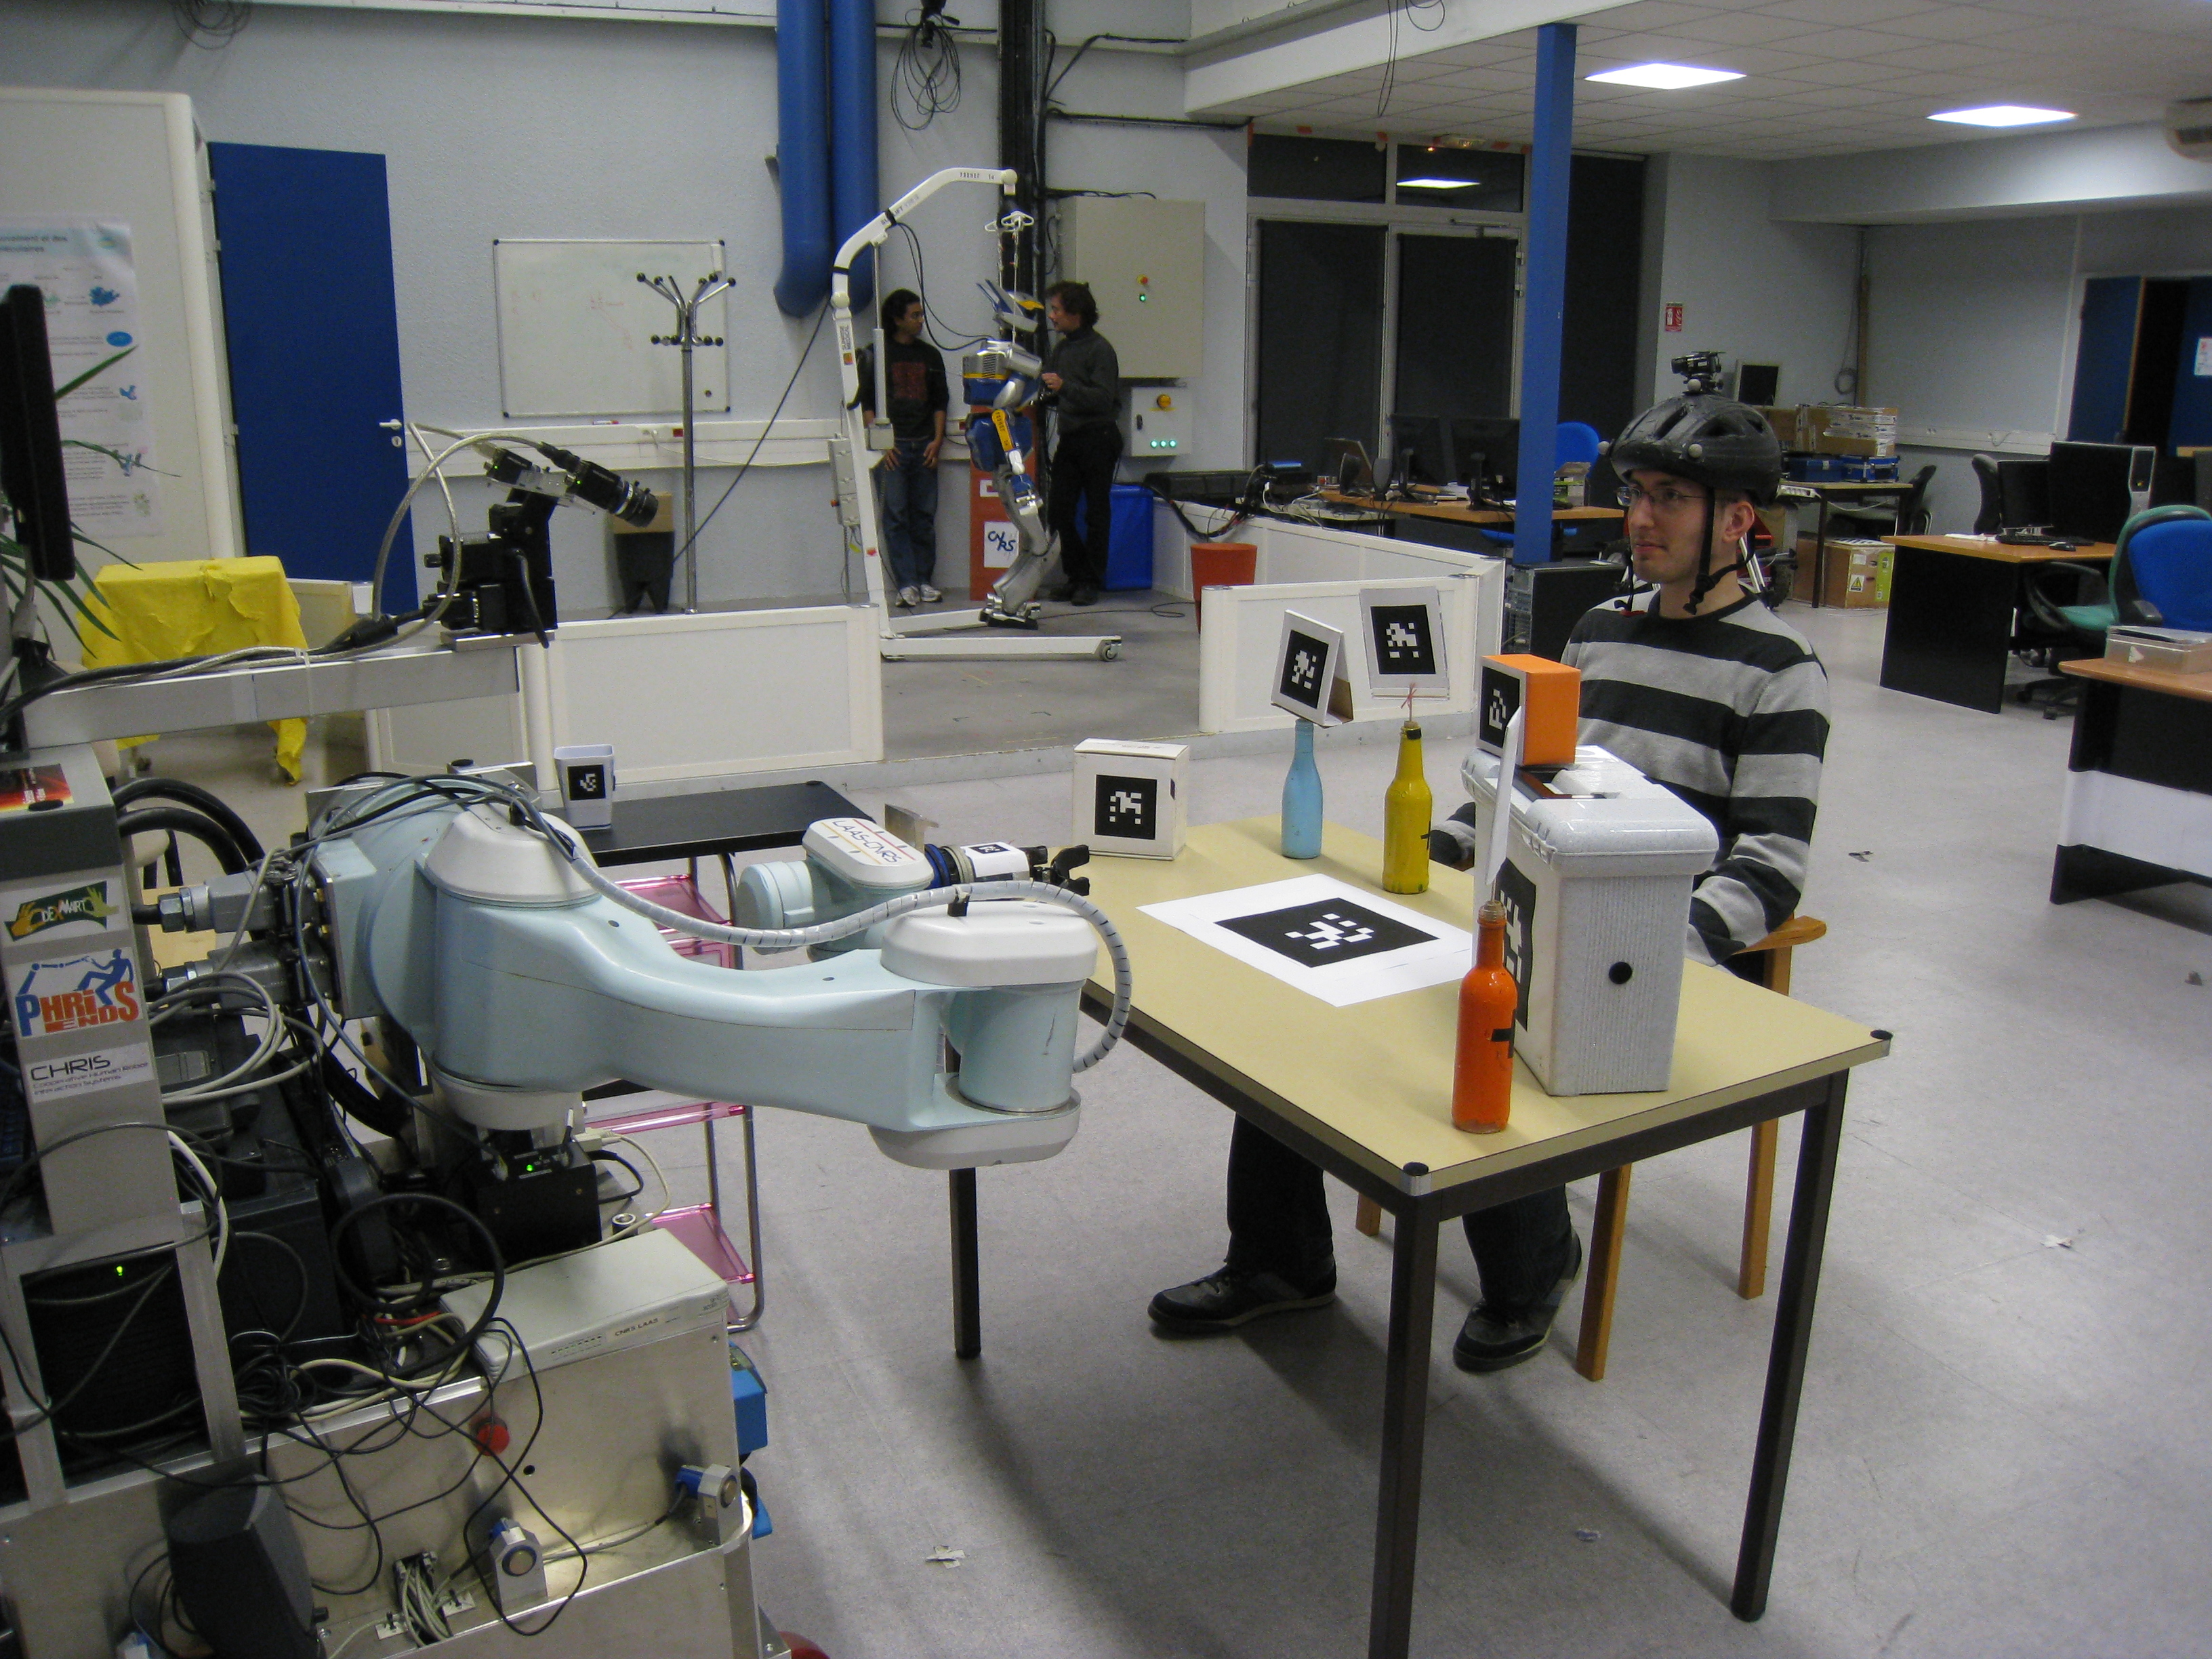
\includegraphics[width=4.3cm]{figs/spy-game-real.jpg}} \hspace{0.2em}
%%\parbox[c]{4.1cm}{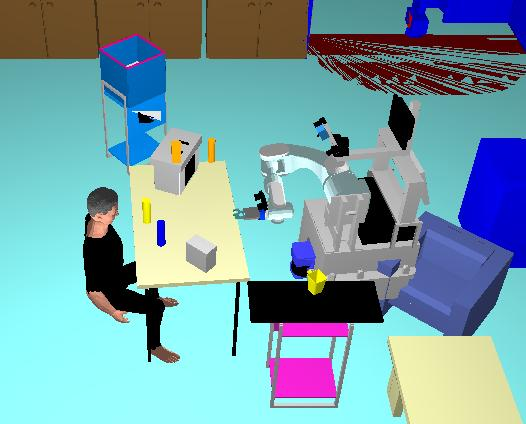
\includegraphics[width=4.1cm]{figs/spy-game-mhp.jpg}}
%\flushleft
%\hspace{1.8cm} (a) \hspace{3.9cm} (b)
%\caption{Spy game scenario: (a) Real environment and (b) 3D environment model, viewed in \textsc{SPARK}.}
%\label{fig|spyGameScenario}
%\end{figure}

%The scenario for this game (Figure~\ref{fig|spyGameScenario}) consists on a
%face-to-face interaction where the human thinks of an object present in the
%environment, while the robot queries the human until either discovering the
%object or giving up~\cite{Ros2010a}. The game starts with the human user giving a
%first hint (communication is done through a keyboard and screen), allowing the
%robot to start the search filtering those objects that fulfill this first
%description. Based on this subset, ORO provides a descriptor (or set of
%descriptors) that allows maximum discrimination among objects in the subset.
%The robot queries the user about the value of the descriptor (or the most
%discriminant among the set of descriptors) and with this new information, the
%current subset of objects is filtered again. The process is repeated until
%either obtaining a single object that fulfills all the descriptor values, or
%failing (\ie no object found). 

%%\begin{figure}%[!ht]
%%\centering
%%\begin{scriptsize}
%%\begin{tikzpicture} %[level/.style={sibling distance=30mm/#1},scale=0.8]
%%	%[edge from parent fork down,
%%	%every node/.style={fill=black!30,rounded corners},
%%	%[parent anchor=east,child anchor=west,grow=east,
%%	%edge from parent/.style={thick,draw}]
%%	\node {Artifact}
%%	child {node {Tableware}
%%		child {node {Bottle}}
%%		child {node {Cup}}
%%		}
%%	child {node {GameObject}}
%%	child {node {Furniture}
%%			child {node {Table}}
%%			child {node {Chair}}
%%			child {node {Shelf}}};
%%\end{tikzpicture}
%%\end{scriptsize}
%%\caption{Example of object categorization used in the scenario.}
%%\label{fig|objectsSpyGame}			
%%\end{figure}

%%Thing
%%Object
%%Tableware
%%	- bottle: red, blue, yellow orange
%%	- cup: white
%%Furniture
%%	- table: hrp2table, lowtable
%%	- chair: chair1 and chair2
%%	- shelf: pink_shelf
%%GameObject: spacenavbox, orangebox, accesskit

%We have integrated the game on the LAAS-CNRS Jido robot.
%Objects are identified through a tag-based vision approach\footnote{ARToolKit:
%\url{http://www.hitl.washington.edu/artoolkit/}} and motion capture is used for
%human tracking. Their descriptions regarding categories (type of object) and
%features (color, shape) are manually given in advance. Spatial relationships
%(\concept{front}, \concept{back}, \concept{left}, etc, and \concept{in},
%\concept{on} and \concept{next to}) and visibility (only visible objects for
%both agents can be considered in the game) are automatically computed on-line
%by \textsc{SPARK}. Figure~\ref{fig|spyGameExample}
%shows an example of a round game.

%\begin{figure}
%\centering
	%\begin{tabular}{r|p{6cm}}
		%\chatN{human} & It is a tableware.\\
		%\chatN{jido} & \emph{[retrieve possible objects: coke-bottle, yellow-bottle, orange-bottle, cup-with-handle]} \\
	 			%& \emph{[keep visible objects: coke-bottle, yellow-bottle, cup-with-handle]}\\
				%& \emph{[obtain discriminants: type, color.]}\\
				%& Which type of object it is: bottle or cup? \\
		%\chatN{human} & Bottle.\\
		%\chatN{jido} & \emph{[obtain possible objects: coke-bottle, yellow-bottle.]}\\
				%& \emph{[obtain discriminants: color.]}\\
				%& What color is the object: red or yellow?\\
		%\chatN{human} & Red.\\
		%\chatN{jido} & \emph{[obtains possible objects: coke-bottle.]}\\
				%& The object is the Coke bottle!	
	%\end{tabular}\\
	%\caption{Example of the robot playing Spy game.}
	%\label{fig|spyGameExample}
%\end{figure}

%\subsection{\emph{Moving to London} Scenario}

%In order to illustrate some of different reasoning abilities of the robot presented in this paper, we have designed the following
%daily life situation. Tom and Jerry are moving to London, so they are packing
%things in boxes. The scenario takes places in the living room, where Jido is observing while they move things here and there. To assess the
%reasoning abilities of the robot they ask Jido for information (entered through
%keyboard). Ideally, the robot should perform actions when required (\eg
%hand an object when asking ``give me...''). However, since it is out of the
%scope of this work, we do not include any motion from the robot's side. Similar
%to the \emph{Spy Game} scenario, perception of objects is done through a tag-based
%system and humans are detected through motion capture. We next describe in
%detail three situations where we can follow the internal robot's reasoning and
%the interaction with the users.

%\subsubsection{Initial Situation Assessment}

%\begin{figure*}
%\centering
	%\subfigure[]
	%{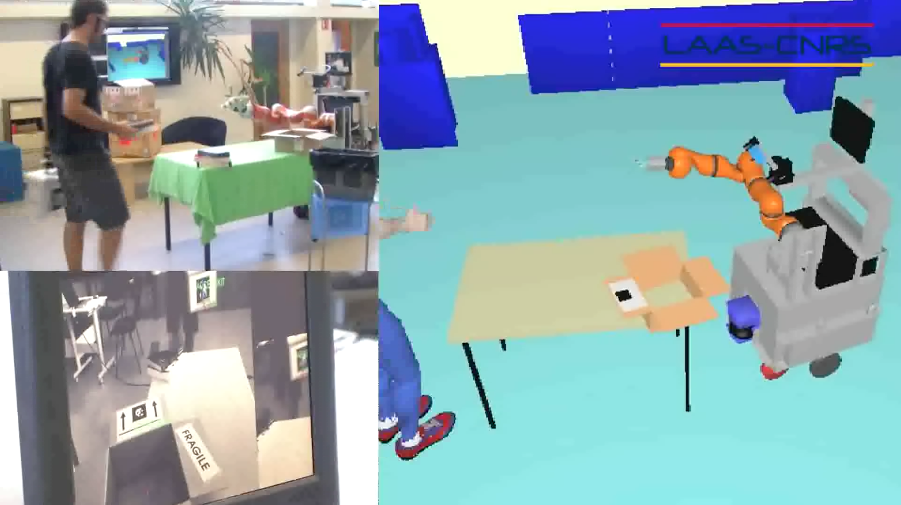
\includegraphics[width=0.3\linewidth]{figs/situationAssessment1.png}\label{(a)}}
	%\subfigure[]
	%{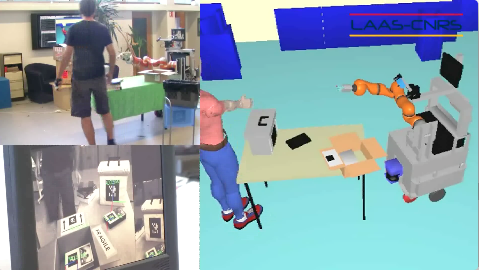
\includegraphics[width=0.3\linewidth]{figs/situationAssessment2.png}\label{(b)}}
	%\subfigure[]
  	%{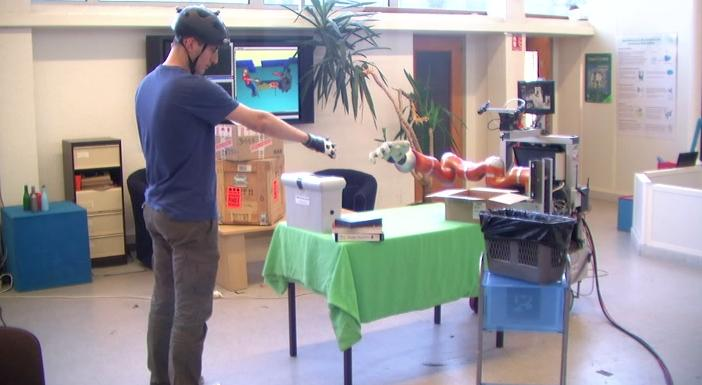
\includegraphics[width=0.3\linewidth]{figs/inTheBox2.jpg}\label{c}}
	%\caption{Situation assessment during initialization (before (a) and after (b) placing the objects on the table). In each image the snapshots correspond to: real environment (top-left sub-image); processed image to identify the tagged objects (bottom-left sub-image); and the 3D environment (right sub-image).(c) Jerry asks Jido for the content of the box while pointing at it.}
	%\label{fig|movingToLondon}
%\end{figure*}

%%\begin{figure}%[!t]
%%\centering
%%  \subfigure[]
%%  {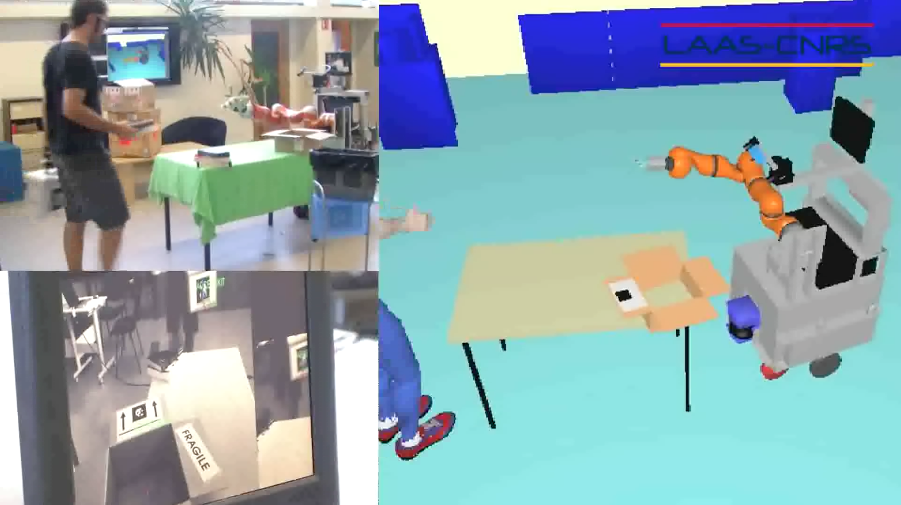
\includegraphics[width=0.95\linewidth]{figs/situationAssessment1.png}\label{a}}
%%  \subfigure[]
%%  {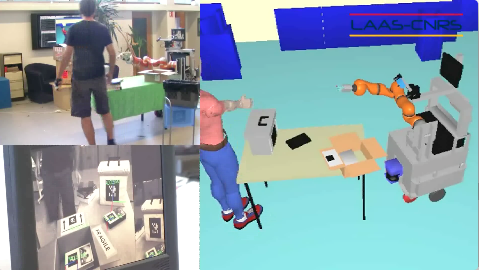
\includegraphics[width=0.95\linewidth]{figs/situationAssessment2.png}\label{b}}
%%	\caption{Situation assessment during initialization: a) before placing the
%%	objects on the table, and b) after placing them. In each image the snapshots
%%	correspond to: real environment (top-left sub-image); processed image to
%%	identify the tagged objects (bottom-left sub-image); and the 3D environment
%%	(right sub-image).}
%%	\label{fig|sitAssessRoman}
%%\end{figure}

%First Tom enters the room with some of the things they need to pack: a
%toolbox and two videos. He leaves one of the video tapes (``Jido-E'') inside one of
%the boxes (the cardboard box), and the other one (``Lord of the Robots'') on the
%table. We next describe how the situation assessment takes place at each step, \ie how the
%ontology is updated with the information obtained from the geometric reasoner
%SPARK.
%The initial information in ORO corresponds to:
%\begin{center}
    %\begin{tabular}{ll}
      %\stmt{table type Table} & \stmt{Tom type Human}\\
      %\stmt{cardBoardBox type Box} & \stmt{Jerry type Human}\\
      %\stmt{toolbox type Box} & \stmt{videoTape1 type VideoTape}\\
      %\stmt{videoTape2 type VideoTape} & \stmt{videoTape2 label "Jido-E"}   
      %\end{tabular}
      %\stmt{videoTape1 label "Lord of the Robots"}
%\end{center}
%\vspace{0.10cm}
	%SPARK detects that there is a cardboard box on the table. It thus sends the fact to ORO:

%\begin{center}
    %\begin{tabular}{l}
      %\stmt{cardBoardBox isOn table}
    %\end{tabular}	             
%\end{center}
%Tom enters carrying several objects (Figure~\ref{fig|movingToLondon}a) and places them around. Then he leaves. (Figure~\ref{fig|movingToLondon}b). The following facts are computed and sent to ORO:
%\begin{center}
    %\begin{tabular}{ll}
      %\stmt{toolbox isOn table} & \stmt{toolbox isNextTo videoTape1}\\
      %\stmt{videoTape1 isOn table} & \stmt{videoTape2 isIn cardBoardBox}
      %\end{tabular}
      %\stmt{videoTape1 isNextTo toolbox}
%\end{center}

%\subsubsection{Implicit Disambiguation Through Visual Perspective Taking}
%\label{exp:disambVPT}

%Tom enters the room again while carrying a big box (Figure~\ref{fig|vpt}). He
%approaches the table and asks Jido to handle him the video tape: ``Jido, can
%you give me the video tape''. The \textsc{Dialogs} module queries the ontology to
%identify the object the human is referring to:
%\begin{center} 
%\stmt{?obj type VideoTape} 
%\end{center}
%There are two video tapes in the scene: one on
%the table, and another one inside the cardboard box. Thus, the knowledge 
%base returns both: 
%\begin{center}
%\hspace{0.7cm}$\Rightarrow$ \concept{?obj = [videoTape1, videoTape2]}
%\end{center}
%However, only one is visible for Tom (the one on the
%table). Thus, although there is an ambiguity from the robot's perspective
%(since it can see both video tapes), based on the perspective of its human
%partner it infers that Tom is referring to the video tape on the table, and not
%the one inside the box which is not visible from his view. Therefore,
%non-visible objects are removed obtaining:

%\begin{center}
%\concept{?obj = [videoTape1]}
%\end{center}

%Since only one object is available now, the robot infers
%that the human refers to it and can eventually execute the command, \ie give
%it to the human. Alternatively, the robot could first verify with the human whether
%that was the object being referred to before proceeding to execute the
%action. Table~\ref{table|ptbeliefs} lists the robot's beliefs about itself and
%its human partner involved in this situation.

%\begin{table}
%\begin{center}
%\begin{tabular}{l}
%\hline
%Robot's beliefs about itself (\emph{robot's model}):\\
%\hline
  %\hspace{0.7cm}\stmt{videoTape1 type VideoTape}\\
  %\hspace{0.7cm}\stmt{videoTape1 isOn table}\\
  %\hspace{0.7cm}\stmt{videoTape1 isVisible \textit{true}}\\
  %\hspace{0.7cm}\stmt{videoTape2 type VideoTape}\\
  %\hspace{0.7cm}\stmt{videoTape2 isIn cardBoardBox}\\
  %\hspace{0.7cm}\stmt{videoTape2 isVisible \textit{true}}\\
%\hline
%\hline
%Robot's beliefs about Tom (\emph{Tom's model}):\\
%\hline
  %\hspace{0.7cm}\stmt{videoTape1 type VideoTape}\\
  %\hspace{0.7cm}\stmt{videoTape1 isOn table}\\
  %\hspace{0.7cm}\stmt{videoTape1 isVisible \textit{true}}\\
  %\hspace{0.7cm}\stmt{videoTape2 type VideoTape}\\
  %\hspace{0.7cm}\stmt{videoTape2 isIn cardBoardBox}\\
  %\hspace{0.7cm}\stmt{videoTape2 isVisible \textit{false}}\\
 %\hline
%\end{tabular}
%\end{center}
%\caption{Robot's beliefs about itself and its human partner.}
%\label{table|ptbeliefs}
%\end{table}

%\subsubsection{Explicit Disambiguation Through Verbal Interaction and Gestures}
%\label{disamb-gestures}

%%\begin{figure}%[!ht]
%%  \centering
%%  \subfigure[]
%%  {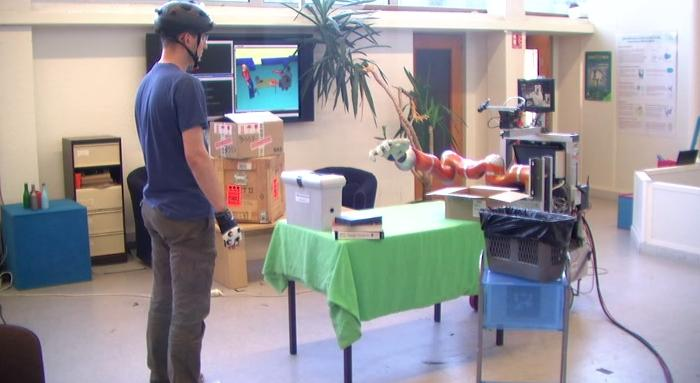
\includegraphics[width=0.9\linewidth]{figs/inTheBox1.jpg}\label{a}}
%%  \subfigure[]
%%  {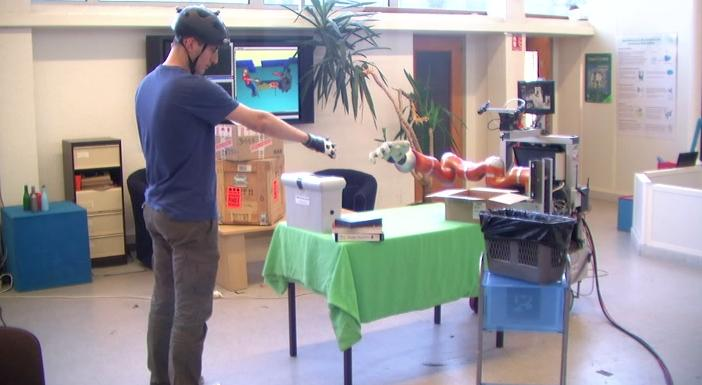
\includegraphics[width=0.9\linewidth]{figs/inTheBox2.jpg}\label{b}}
%%\caption{(a) Jerry asks Jido for the content of the box and (b) points at it.}
%%  \label{fig|pointing}
%%\end{figure}

%In this last situation Jerry enters the
%living room without knowing where Tom had placed the video tapes. So he first
%asks Jido: ``What's in the box?''. Before the robot can answer the question it
%has to figure out which box Jerry is talking about. Similar to the previous
%situation, there are two available boxes: 
%\begin{center}
%\begin{tabular}{l}
%\stmt{?obj type Box}\\
%\hspace{0.7cm}$\Rightarrow$ \concept{?obj = [cardBoardBox, toolbox]}
%\end{tabular}
%\end{center}
%However both are visible and the cognitive ambiguity resolution cannot be
%applied. The only option is to ask Jerry which box he is referring
%to\footnote{Note that Jerry is using the definite article \emph{the}: the robot
%has to determine which box is relevant. {\sc Dialogs} supports other kinds of
%quantification (existantial -- \emph{some} --, universal -- \emph{all} -- , explicit cardinality), as expressed by the combination of definite/indefinite and
%singular/plural forms of articles.}: ``Which box, the toolbox or the cardboard box?''
%Jerry could now simply answer the question. Instead, he decides to point at it
%while indicating: ``That box'' (Figure~\ref{fig|movingToLondon}c). The robot's
%perception identifies the {\tt cardBoardBox} as being pointed at and looked
%at by the human and updates the ontology with this new information using a
%rule available in the commonsense ontology:
%\begin{center}
%\begin{tabular}{r}
%\stmt{Jerry pointsAt carboardBox}, 
%\stmt{Jerry looksAt carboardBox}\\
%$\to$ \stmt{Jerry focusesAt carboardBox}\\
%\end{tabular}
%\end{center}
%In the meantime, the \textsc{Dialogs} module is processing the human verbal input. When trying to resolve the reference ``that'' it is able to merge\footnote{Due to synchronization issues, the user should perform the gesture (pointing at) before answering the robot's question and maintain it until the resolution process takes place.} both sources of information, verbal and gestural, to distinguish the box Jerry refers to:
%\begin{center}
%\begin{tabular}{l}
%\stmt{Jerry focusesAt ?obj}\\
%\hspace{0.7cm}$\Rightarrow$ \concept{?obj = [cardBoardBox]}
%\end{tabular}
%\end{center}

%Finally, \textsc{Dialogs} queries the ontology about the content of the box
%and the question can be answered: ``Jido-E''. Note that the object's label is
%used instead of its ID. This way we enhance interaction using familiar names
%given by the users:
%\begin{center}
%\begin{tabular}{l}
%\stmt{?obj isIn cardBoardBox}\\
%\hspace{0.7cm}$\Rightarrow$ \concept{?obj = videoTape2}\\
%\end{tabular}
%\end{center}

%At this point Jerry wants to know where the other video tape is, and that is exactly
%what he asks Jido: ``And where is the other video tape?''. In this occasion, the
%\textsc{Dialogs} module is able to interpret that Jerry is not referring to the
%video tape which they were just talking about, but to the other one:
%\begin{center}
%\begin{tabular}{l}
%\stmt{?obj type VideoTape}\\
%\stmt{?obj differentFrom videoTape2}\\
%\hspace{0.7cm}$\Rightarrow$ \concept{?obj = [videoTape1]}
%\end{tabular}
%\end{center}

%Since there is only one possible ``other'' video tape (there are only two video tapes in
%the scene), it can directly answer Jerry: ``The other video tape is on the table and
%next to the toolbox.''
%\begin{center}
%\begin{tabular}{l}
%\stmt{videoTape1 isOn table}, 
%\stmt{videoTape1 isNextTo toolbox}
%\end{tabular}
%\end{center}



%%%%%%%%%%%%%%%%%%%%%%%%%%%%%%%%%%%%%%%%%%%%%%%%%%%%%%%%%%%%%%%%%%%%%%%%%%%%
%%%%%%%%%%%%%%%%%%%%%%%%%%%%%%%%%%%%%%%%%%%%%%%%%%%%%%%%%%%%%%%%%%%%%%%%%%%%

\section{An illustrative example}\label{sec:expes}

We assume here that the robot (and the human) has been given the joint goal
``CLEAN TABLE''. For HATP, this means putting all tapes that are
currently on the table in the trashbin. Depending on the state of the
world and agent preferences, different plans are produced.

Figure~\ref{plan-etat2} shows a plan produced to clean the table based on the initial the initial state given in  \S~\ref{sub:gtrc}.

\begin{figure*}[thpb]
  \centering
  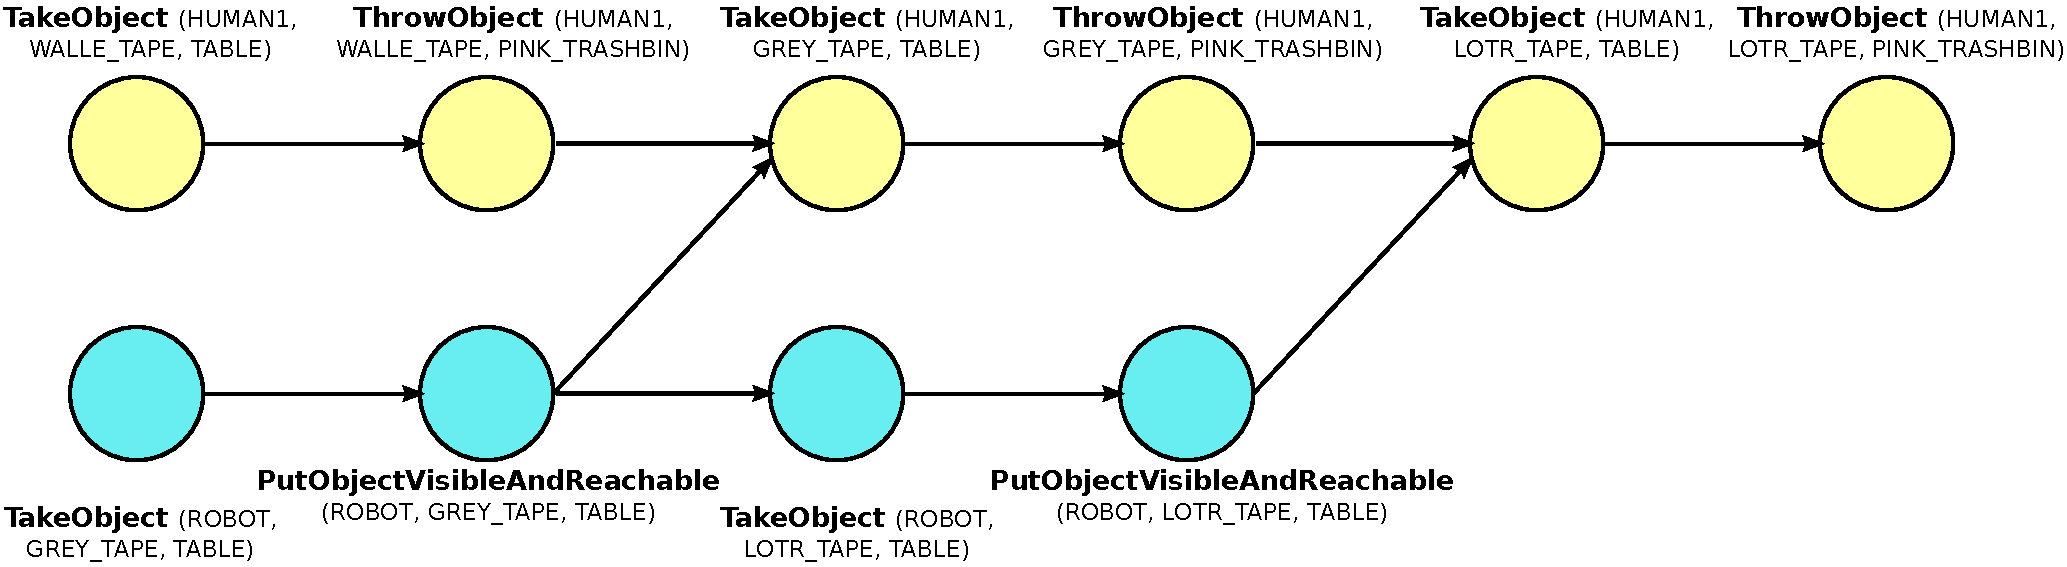
\includegraphics[width=1.0\textwidth]{./figs/plan3.pdf} \\
  \caption {A plan produced by HATP for clean the table based on the initial state given in \S~\ref{sub:gtrc}}
  \label{plan-etat2}
\end{figure*}

Let us now take a simpler example to illustrate a full run of the
system. We have only one tape on the table and it is is reachable only
by the robot while the throw position on top of the trashbin is
reachable only by the human.

% \begin{landscape}
% \begin{figure*}[thpb]
%   \centering
% %  \includegraphics[width=1.0\textwidth]{./figs/manip_run.pdf} \\
%   \includegraphics[width=17cm]{./figs/manip_run.pdf} \\
% \begin{center}
%   \caption {An example of a human-robot collaborative goal achievement}
% \end{center}
%   \label{manip_run_fg}
% \end{figure*}
% \end{landscape}

\begin{figure*}[thpb]
  \centering
\includegraphics[width=1.0\textwidth]{./figs/rotated-rachid_manip_run-v2.pdf} \\
%  \includegraphics[width=17cm]{./figs/manip_run-vertical.pdf} \\
\begin{center}
  \caption {An example of a human-robot collaborative goal achievement}
\end{center}
  \label{manip_run_fg}
\end{figure*}


%\subsection{successful execution}

Figure~\ref{manip_run_fg} illustrates the main processes occurring
during a multi-step human-robot collaborative goal achievement.  The
plan produced is quite straightforward and is shown in the third row
called ``Goal and Plan''. It consists in 4 successive actions
involving the robot and the human. Robot grasps the tape and then
places it on the table at a position where it is visible and reachable
for the human. Human then is asked to pick the tape and throw it in
the trashbin. The first row, named ``Cameras'', shows several
snapshots corresponding to various execution steps. Snapshot~1
presents the initial situation. Snapshots~2, 3, 4 and 5 give the state
after the successive achievement of the four actions in the plan. The
second row, named ``3D Model'', shows the display of SPARK at the same
instants. The fourth, row called ``Robot Speech Acts'', gives robot
speech acts produced along the execution to inform the human partner
about goal and plan creation and status and to verbalize the actions
that the human is asked to execute. The fifth row illustrates robot
knowledge on itself and on the objects. The sixth row illustrates the
robot knowledge about the human state. The seventh row gives ongoing
robot action with action preconditions and effects assessment as well
as motion execution tasks. Motion trajectory typology can be found
between the 3D Model views. The eighth row gives ongoing human action
with action preconditions and effects assessment and monitoring
activity.



%%%%%%%%%%%%%%%%%%%%%%%%%%%%%%%%%%%%%%%%%%%%%%%%%%%%%%%%%%%%%%%%%%%%%%%%%% 
%%%%%%%%%%%%%%%%%%%%%%%%%%%%%%%%%%%%%%%%%%%%%%%%%%%%%%%%%%%%%%%%%%%%%%%%%% 

\section{Conclusion}
\label{conclusion}

\subsection{Towards an Event-Driven, Knowledge-Oriented Architecture for Personal Robotics}

In this paper, we have studied knowledge streams between three components: {\it(1)}
{\sc ORO}, an ontology-based knowledge server that stores and maintains
classified RDF statements produced by other modules in agent-specific
models and allows information to be easily retrieved, either through queries or
via an event system; {\it(2)} {\sc SPARK}, the grounded, human-aware 3D model
of the environment that performs all the spatial reasoning within our
architecture, including reasoning involving motion planing (to compute
reachability of objects) and perspective taking, and {\it(3)} {\sc Dialogs}, a
natural language processor that performs simple grammatical parsing of English
language, grounds the semantic content of the utterance (if necessary, also
interacts with the user to disambiguate), and eventually generates a RDF
representation of the sentence.

These components, combined with modules dedicated to symbolic supervision and
task planning (these modules are outside of the scope of this article), compose
an architecture that we call \emph{knowledge-oriented}:

\begin{itemize}
\item{Knowledge is explicitly stored in one central and consistent repository
of facts, accessible by all modules.}
\item{Knowledge is represented in a strict formalism (OWL statements) and
with a clearly defined vocabulary (stated in the {\tt commonsense.oro.owl}
ontology).}
\item{The first two points enable both a loosely-coupled
architecture where modules can very easily be removed or replaced by other ones
as long as they share the same semantics (modules are defined by the knowledge
they produce),}
\item{and a \emph{symbolic} reactive, event-driven approach
to supervision. By managing events at the same level as
the reasoner, we take full advantage of the inference abilities of ORO to
trigger events whose \texttt{true} conditions can be inferred.}
\item{Finally, this architecture allows for the combination of very different knowledge
modalities in a single homogeneous environment, bringing mutual benefits to
components. For instance, the dialogue processing module can perfectly run
without any geometric perception, but its disambiguation routines can
transparently benefit from it when available (since richer symbolic
descriptions of objects are then available).}
\end{itemize}

This architecture moves away from standard layered approaches. Interactions
between components are mostly bidirectional and we do not have a concept of
layers of abstraction (we do, however, have access to the lower level modules
of the robot to execute actions, but all cognition-related modules reside at the
same level). This is especially visible for the dialogue input processing. This
component does not simply act as an alternative perceptual input to the
symbolic database, but also actively queries previously acquired knowledge to
disambiguate and validate the newly created symbolic knowledge.


Regarding the anchoring question, this architecture is
bidirectional. The components we described provide a \textit{bottom-up}
grounding process: SPARK and \textsc{Dialogs} constantly build and push new
symbolic contents about the world to ORO where it becomes accessible to
decisional layers. In parallel, ORO relies on reasoning in a \textit{top-down}
way to produce new facts that may trigger in return physical behaviours. 

% We believe that this \emph{knowledge-oriented} approach has a strong potential
% not only to enable rich human-robot interaction, but also as a broader approach
% to information alignment and fusion in complex robotic systems.  The
% versatility of this paradigm could be illustrated by a simple imaginary
% scenario with a blind robot and a deaf robot. The blind robot does not see (no
% cameras or alike), but someone can verbally describe a scene to it. On the
% other hand, the deaf robot has a good vision system, but cannot hear.  Without
% any changes to the software architecture described, supervision modules of both
% robots would be able to perform equally well.

%(to actually implement this imaginary
%situation, the blind robot would of course need \textit{a priori} 3D models
%of objects talked about to enable planning or pick and place actions, and
%the deaf robot would require at least some gesture interpretation to
%understand orders).

% We hope as well that our contribution may contribute to fill the gap between
% robotics and psychology. Our architecture provides easier-to-reach entry points
% to implement some classical psychology tests to robots. We presented
% experiments focused on issues related to perspective taking. By explicitly
% enabling independent modeling of the beliefs of each agent, our architecture is
% especially well suited to set up cognitive and psychological experiments (such
% as the \emph{False-Belief} experiment), which we plan to
% further explore.

\subsection{Discussion}

Our system has however shortcomings and opens several questions on different
topics.  In this section, we discuss some of these limitations, possible
extensions, and how this article contributes to the larger debate on symbol
grounding for embodied agent.

\subsubsection{Modeling the Real World}
\label{modeling_real_world}

The main challenge we address in this work can be formulated as \emph{How to
model real-world interaction in a symbolic way, processable by the robot to
make decisions}. In the paper we used several times the term \emph{grounding} to
describe the process of binding percepts to symbols (later organized in a
first-order logic framework).  We would like to relate it to
Sloman's~\cite{Sloman2007} stance against the \emph{``Symbol Grounding meme''},
where he argues that symbolic grounding is bound to the representation of
somatic concepts (\ie roughly, the sensori-motor relationships that the robot
learns from its interaction with the world) which in turn severely constraints
the domain of concepts accessible to the robot. We could call this type of
grounding \emph{bottom-up} grounding, and Steels~\cite{Steels2007} claims it is
a solved issue.

For us, \emph{grounding} is on the contrary a \emph{top-down} activity: the
robot needs to automatically bind a representation (for instance, a word
uttered by a human, an image taken from a camera, a sentence extracted from
Wikipedia) to an unambiguous, context-dependent, internal concept. This 
concept may (or may not) be \textit{a priori} available to the robot as a
pre-loaded ontology (what we previously called the cultural background of the
robot).

Note also that perception issues have been solved in our experiments by using a tag-based object identification
method. In section~\ref{informational_content_extraction} we give an example
where the human says ``the yellow banana is big''. It is assumed in the example
that the robot already knows about a banana instance that is yellow. In our
experiments, this kind of knowledge was either hard coded in scenario-specific
ontologies (\eg \stmt{banana\_01 type Banana} where \concept{banana\_01}
is the id of the banana's tag) or taught to the robot with prescriptive
sentences like ``Learn that this is a banana'' while pointing at the banana's
tag. It would be interesting to extend this approach with automatic classifiers
(for colour, size, etc.). If the robot later discovers a yellowish and large
object, an utterance like ``the yellow banana is big'' could be used to assert
that this object is a banana.  A similar approach focused on the combination of visual perception and communication modalities to achieve visual learning has been 
developed by~\cite{Vrecko2009}.

While the examples we develop are all based on symbols that have a physical
meaning, the system deals equally well with abstract, \emph{exo-somatic},
concepts like \emph{Time}, \emph{Event} or \emph{Place}. Demonstrating this in
real experiments would be an interesting development.

Amongst the other shortcomings of our architecture, neither the \emph{domain of
validity} nor the context of a fact are represented in a satisfying way (we do
store some kind of context --the agent's mental model for instance). This
information is meta-information on the knowledge. While the ORO framework
allows them through \emph{statement reification}, it does not offer yet a
convenient way to store them. One obvious limitation that derives from the lack
of efficient meta-knowledge is the absence of knowledge history.  With ORO, the
robot always lives in the present.

Along the same lines, our current framework lacks a proper management of
uncertainty which is essential for real world environments. A probabilistic
layer should be added by attaching truth probabilities to statements, similar
to~\cite{Jain2009}.

% 
% \subsubsection{The challenge of natural language parsing}
% 
% \fxfatal{in Dialogs, no correct/systematic processing of illocutionary acts
% like "learn", "stop" -> that would be the role of the content analysis}
% \fxfatal{mention type of speech act we don't handle}
% 
% \subsubsection{Action recognition and assessment of non-verbal communication}
% 
% \fxfatal{situation assessment: we don't do any posture, gesture recognition, let be action recognition}
% 

\subsubsection{On Thematic Roles and Action Models}

The current implementation relies on a small, predefined set of action verbs that can
be recognized from natural language (section~\ref{processing_of_actions}).
This constraint does not come from the resolution algorithm itself, but
rather from the difficulty to automatically extract the thematic roles associated
to a verb. 
This could be improved by linking a symbolic task
planner to the \textsc{Dialogs} module to dynamically provide the list of
actions that the robot can process, \ie actions for which the robot can produce
a plan. Additionally, we could exploit on-line resources like
\textsc{VerbNet}~\cite{Kipper2008}, which provides a large machine-processable
lexicon of English verbs along with their thematic roles.

\subsubsection{Knowledge and Embodiment}

The three experiments that were presented in the paper all illustrate how the
robot makes use of its embodied nature to establish a meaningful communication
with a human. Mainly, because the robot and the human share the same physical
environment and they perceive each other, we are able to create a mutual
context.

Sloman, in~\cite{Sloman2009}, argues however that the strong focus on
embodiment in the robotics community has hindered progress towards natural
human-robot interaction. Our approach has hopefully made clear that, similar to
Beetz et al.~\cite{Beetz2010}, we do not consider embodiment \emph{per se} outside of
a broader symbolic system, \ie our architecture is not bound to the morphology or
the low-level sensori-motor capabilities of a specific agent. 

However, we can build a model of the ``human point of view'' because the robot
perceives the human, and is able to estimate, at least partially, what the
human perceives or not. We infer that a human focuses on some object because
he/she points at it, looks at it, and besides, the object is visible to him.
This relies on the embodied nature of the interaction. In turn, this allows us
to understand the meaning of sentences like ``Give me that''.

We hope that this contribution shows that considering embodiment as the most
challenging and fruitful characteristic of robotics in regards to the whole AI
community does not contradict with a formal, highly symbolic approach of the
representation and decision problems that arise in robotics. 

Let us conclude this article briefly reviewing and linking Roy's list of challenges
for human-robot dialogue with our current approach: 
\begin{itemize}

	\item While more modalities (especially, deictic gestures and social gazes)
	can be added, we have actually proposed a \emph{cross-modal
	representation system}.

	\item One of the main feature of the \textsc{Dialogs} module is its ability
	to interactively ground concepts through disambiguation, bringing the
	ability for the robot to \emph{associate words with perceptual and action
	categories}.

	\item The ORO knowledge base offers some support for the \emph{modeling of
	context}, but a lot remains to be done in this respect.

	\item \emph{Figuring out the right granularity of models} is partially
	solved by supporting both a geometric reasoning level and a purely symbolic
	level. Generally speaking, it appears that complex robotic systems need
	to operate with a dynamic granularity, depending on the task to achieve.

	\item \emph{Temporal modeling} is currently missing in our architecture,
	and symbolic and geometric \emph{planning} is accomplished outside of the
	knowledge representation loop we presented here. We see planning as an
	essential tool to build predictive knowledge, and we are looking into this
	direction.

	\item Since we provide no time management, our system is currently not able
	to \emph{match past (learned) experiences with the current interaction}.
	This ability is obviously a key step for general action recognition, and
	seems of particular importance for the robot to assess the state of the
	interaction with the human.

	\item Finally, Roy mentions \emph{the ability to take into account the
	human perspective}: this is probably our main contribution which we are now
	trying to develop even further towards psychology-inspired experiments.

\end{itemize}




%%%%%%%%%%%%%%%%%%%%%%%%%%%%%%%%%%%%%%%%%%%%%%%%%%%%%%%%%%%%%%%%%%%%%%%%%% 
%%%%%%%%%%%%%%%%%%%%%%%%%%%%%%%%%%%%%%%%%%%%%%%%%%%%%%%%%%%%%%%%%%%%%%%%%% 

\bibliographystyle{spbasic}
\bibliography{chapter}


%%%%%%%%%%%%%%%%%%%%%%%%%%%%%%%%%%%%%%%%%%%%%%%%%%%%%%%%%%%%%%%%%%%%%%%%%% 
\end{document}

